\documentclass[12pt]{article}
\usepackage{times}
%\usepackage{palatino}
%\usepackage{fourier}  % Looks nice but isn't present in many LaTeX distros.
\usepackage[T1]{fontenc}
\usepackage{amsmath,amsbsy,amssymb}
\usepackage{deflist}
%\usepackage{fancyheadings}
\usepackage{fancyhdr}
\usepackage{colortbl}
\usepackage{color}
\usepackage[table]{xcolor}

\usepackage{fancybox}

\usepackage{tabularx}
\usepackage{verbatim}
\usepackage{moreverb}
\usepackage{float}
\usepackage{graphicx}
\usepackage{longtable}
\usepackage{subfigure}
%\usepackage{ssss}
\usepackage{fancybox}
\usepackage{booktabs}
\usepackage{array}
%\usepackage{toc_entr}

\definecolor{lightgray}{gray}{0.9}
\definecolor{lightblue}{rgb}{0.93,0.95,1.0}
\definecolor{lightteal}{rgb}{0.95, 1.38, 1.39}

%\usepackage[framemethod=tikz,outerlinewidth=2,outerlinecolor=blue,backgroundcolor=lightblue]{mdframed}
\usepackage[framemethod=tikz,outerlinewidth=2,outerlinecolor=teal,backgroundcolor=lightteal]{mdframed}

%\usepackage[tikz]{bclogo}

\usepackage[debug=false, colorlinks=true, pdfstartview=FitV, linkcolor=teal, citecolor=black, urlcolor=green]{hyperref}

\textwidth 6.5in
\textheight 9.5in
\topmargin -1.0in
%\topmargin -3.280cm
\newlength{\boxwidth}
\setlength{\boxwidth}{5.8in}
\oddsidemargin 0.in
\evensidemargin 0.in
\headheight 0.25in
\lhead{\sl PFLOTRAN: Quick Reference User Guide}
\chead{\sl DRAFT}
\chead{\S\arabic{section}.\arabic{subsection}.\arabic{subsubsection}}
%\rhead{DRAFT \qquad \qquad \ \today}
\rhead{\today}
%\rfoot{\today--[\thepage]}
\rfoot{}
\cfoot{\rm < \thepage\ >}
%\cfoot{}
%\footrulewidth 0.4pt
\newcommand\keyend{{(END \, / \, .)}}
\newcommand\return{{\hfill$\hookrightarrow$} Return to Keyword List}
\newcommand\returnb{{\hfill$\nearrow$}}
%\newcommand\return{{\hfill\bf RETURN}}

\newcommand{\negsp}{\vspace{-4mm}}
\newcommand\secsp{\vspace{-3 mm}}
\newcommand\secspb{\vspace{-2 mm}}
\newcommand\subsecsp{\vspace{-0.0 mm}}
\newcommand\pflotran{{\bf\sl PFLOTRAN}}
\newcommand\pflow{{\bf\sl PFLOW}}
\newcommand\ptran{{\bf\sl PTRAN}}
\renewcommand{\baselinestretch}{1.01}
%\setlength{\baselineskip}{13pt}
\def\EQ#1\EN{\begin{equation}#1\end{equation}}
\def\BA#1\EA{\begin{align}#1\end{align}}
\def\BS#1\ES{\begin{split}#1\end{split}}
%\newcommand{\EQ}{\begin{equation}}
%\newcommand{\EN}{\end{equation}}
\newcommand{\longline}{\noindent\rule[-0.1in]{\textwidth}{0.01in}}
\newcommand{\bc}{\begin{center}}
\newcommand{\ec}{\end{center}}
\newcommand{\degc}{$^\circ$C}
\newcommand{\eq}{\ =\ }
\newcommand{\eff}{{\rm eff}}
\newcommand{\eqr}{{\rm le}}
\newcommand{\equ}{{\rm eq}}
\newcommand{\kin}{{\rm kin}}
\newcommand{\rdx}{{\rm rdx}}
\newcommand{\ind}{{\rm id}}
\newcommand{\dep}{{\rm dp}}
\newcommand{\e}{{\rm{e}}}
\newcommand{\erf}{{\rm{erf}}}
\newcommand{\erfc}{{\rm{erfc}}}
\renewcommand{\sc}{{\rm sc}}
\newcommand{\sign}{{\rm{sign}}}
\newcommand{\p}{{\partial}}
\newcommand{\im}{{\rm im}}
\newcommand{\m}{{\rm m}}
\newcommand{\A}{{\mathcal A}}
\newcommand{\B}{{\mathcal B}}
\newcommand{\C}{{\mathcal C}}
\newcommand{\D}{{\mathcal D}}
\newcommand{\E}{{\mathcal E}}
\newcommand{\F}{{\mathcal F}}
\newcommand{\G}{{\mathcal G}}
\newcommand{\J}{{\mathcal J}}
\newcommand{\jo}{{j_o}}
\newcommand{\M}{{\mathcal M}}
\newcommand{\N}{{\mathcal N}}
\newcommand{\mO}{{\mathcal O}}
\renewcommand{\P}{{{\mathcal P}}}
\newcommand{\Q}{{\mathcal Q}}
\newcommand{\R}{{{\mathcal R}}}
\newcommand{\mcS}{{\mathcal S}}
\newcommand{\T}{{\mathcal T}}
\newcommand{\W}{{\mathcal W}}
\newcommand{\X}{{\mathcal X}}
\newcommand{\Y}{{\mathcal Y}}
\newcommand{\Z}{{\mathcal Z}}
\newcommand{\rev}{{\rm rev}}
\newcommand{\irr}{{\rm irr}}
\renewcommand{\a}{{\alpha}}
\newcommand{\abar}{{\bar \alpha}}
\renewcommand{\b}{{\beta}}
\renewcommand{\c}{{\rm CO_2}}
\newcommand{\w}{{\rm H_2O}}
\newcommand{\air}{{\rm N_2}}
\newcommand{\pe}{{\rm Pe}}
\newcommand{\da}{{\rm Da}}
\renewcommand{\k}{{\dot R}^0}
\renewcommand{\L}{\widehat{\mathcal L}}
\renewcommand{\bar}{\overline}
\newcommand{\dsty}{{\displaystyle}}
\newcommand{\diff}{{\mathcal D}}
\newcommand{\surf}{\equiv \!\!\!}
\newcommand{\bnabla}{\boldsymbol{\nabla}}
\newcommand{\bA}{\boldsymbol{A}}
\newcommand{\ba}{\boldsymbol{a}}
\newcommand{\bB}{\boldsymbol{B}}
\newcommand{\bC}{\boldsymbol{C}}
\newcommand{\bD}{\boldsymbol{D}}
\newcommand{\bE}{\boldsymbol{E}}
\newcommand{\bF}{\boldsymbol{F}}
\newcommand{\bi}{\boldsymbol{i}}
\newcommand{\bI}{\boldsymbol{I}}
\newcommand{\bJ}{\boldsymbol{J}}
\newcommand{\bK}{\boldsymbol{K}}
\newcommand{\bM}{\boldsymbol{M}}
\newcommand{\bg}{\boldsymbol{g}}
\newcommand{\bGamma}{\boldsymbol{\Gamma}}
\newcommand{\bOmega}{\boldsymbol{\Omega}}
\newcommand{\bPsi}{\boldsymbol{\Psi}}
\newcommand{\bO}{\boldsymbol{O}}
\newcommand{\bnu}{\boldsymbol{\nu}}
\newcommand{\bdS}{\boldsymbol{dS}}
\newcommand{\bq}{\boldsymbol{q}}
\newcommand{\br}{\boldsymbol{r}}
\newcommand{\bR}{\boldsymbol{R}}
\newcommand{\bS}{\boldsymbol{S}}
\newcommand{\bu}{\boldsymbol{u}}
\newcommand{\bv}{\boldsymbol{v}}
\newcommand{\bx}{\boldsymbol{x}}
\newcommand{\by}{\boldsymbol{y}}
\newcommand{\bz}{\boldsymbol{z}}
\newcommand{\bzero}{\boldsymbol{0}}
\newcommand{\arrows}{~\rightleftharpoons~}
\newcommand{\arrowstab}{\!\!\!\rightleftharpoons\!\!\!}
\newcommand{\CA}{C_{\rm A}}
\newcommand{\CB}{C_{\rm B}}
\newcommand{\CC}{C_{\rm C}}
\newcommand{\CAB}{C_{\rm AB}}
\newcommand{\CBC}{C_{\rm BC}}
\newcommand{\RA}{\R_{\rm A}}
\newcommand{\RB}{\R_{\rm B}}
\newcommand{\RC}{\R_{\rm C}}
\newcommand{\RAB}{\R_{\rm AB}}
\newcommand{\RBC}{\R_{\rm BC}}
%\newcommand{\kdsc}{K^{DS}}
%\newcommand{\kdec}{K^{DE}}
%\newcommand{\kdsm}{\overline K^{DS}}
%\newcommand{\kdem}{\overline K^{DE}}
\newcommand{\kdsc}{K^{sc}}
\newcommand{\kdec}{K^{ec}}
\newcommand{\kdsm}{K^{sm}}
\newcommand{\kdem}{K^{em}}
\newcommand{\csm}{S}
\renewcommand{\csc}{S}
\newcommand{\cem}{\E}
\newcommand{\cec}{\E}
\renewcommand{\min}{{\rm min}}
\newcommand{\coll}{{\rm coll}}
\newcommand{\ex}{{\rm ex}}
\newcommand{\srf}{{\rm srf}}
\def\dbar{{\mkern2mu\mathchar'26\mkern-11mu\mathrm{d}}}

\renewcommand{\contentsname}{TABLE OF CONTENTS}
\renewcommand{\listfigurename}{{LIST OF FIGURES}}
\renewcommand{\listtablename}{{LIST OF TABLES}}

\renewcommand{\arraystretch}{1.3}

\setlength{\parindent}{0.3125in}
\setlength{\parskip}{2ex plus 0.2ex minus 0.2ex}

\setcounter{secnumdepth}{4}
\setcounter{tocdepth}{4}

\pagestyle{fancy}
%\pagestyle{empty}

\thispagestyle{empty}

%\renewcommand{\theequation}{\arabic{equation}}
%\renewcommand{\thetable}{{\protect\bf\arabic{table}}}
%\renewcommand{\thefigure}{{\protect\bf\arabic{figure}}}
%\renewcommand{\thepage}{\roman{page}}

\renewcommand{\theequation}{\arabic{section}-\arabic{equation}}

\setlongtables

\begin{document}

%begin title page
\begin{comment}
\noindent
{\large\sffamily LA-UR-06-7048}

\medskip

\noindent
\scriptsize
{\em Approved for public release;}\\
{\em distribution is unlimited.}
\end{comment}

\normalsize

\bc
\begin{tabular}{r|l}
~ & ~\\
%{\em Title:} & {\sl Quick Reference Guide: PFLOTRAN 1.0 (LA-CC 06-093)}\\
{\em Title:} & {\sl Quick Reference Guide: PFLOTRAN 2.0 (LA-CC-09-047)}\\
~ & {\sl Multiphase-Multicomponent-Multiscale Massively Parallel} \\
~ & {\sl Reactive Transport Code}\\
~ & ~\\
~ & ~\\
{\em Author(s):} & Peter C. Lichtner (peter.lichtner@gmail.com)\\
~  & Glenn Hammond (glenn.hammond@pnnl.gov)\\
~ & ~\\
~ & ~\\
{\em Contacts:}  & Richard Mills (rmills@ornl.gov)\\
~ & Chuan Lu (Chuan.Lu@inl.gov)\\
%~ & %David Moulton (moulton@lanl.gov)\\
%~ & Bobby Philip (bphilip@lanl.gov)\\
~ & Satish Karra (satkarra@lanl.gov)\\
~ & Jitendra Kumar (jitu1503@gmail.com)\\
%~ & Barry Smith (bsmith@anl.gov)\\
~ & \\%Albert Valocchi (clu@lanl.gov)\\
~ & ~\\
%{\em Submitted to:} & \\
~ & ~\\
{\em Date:} & \today \\
~ & ~\\
~ & ~\\
~ & {\bf \large Work in Progress}\\
~ & ~\\
\end{tabular}
\ec

\vfill

\begin{comment}
\noindent
{\Huge\sffamily Los Alamos}

\vspace{-8pt}

\noindent
{\sffamily NATIONAL LABORATORY}

\vspace{-6pt}

\noindent
\scriptsize
Los Alamos National Laboratory, an affirmative action/equal opportunity employer, is operated by the Los Alamos National Security, LLC
for the National Nuclear Security Administration of the U.S. Department of Energy under contract DE-AC52-06NA25396. By acceptance
of this article, the publisher recognizes that the U.S. Government retains a nonexclusive, royalty-free license to publish or reproduce the
published form of this contribution, or to allow others to do so, for U.S. Government purposes. Los Alamos National Laboratory requests
that the publisher identify this article as work performed under the auspices of the U.S. Department of Energy. Los Alamos National
Laboratory strongly supports academic freedom and a researcher�s right to publish; as an institution, however, the Laboratory does not
endorse the viewpoint of a publication or guarantee its technical correctness.

\hfill Form 836 (7/06)
\end{comment}

\normalsize

\clearpage

\tableofcontents
%\clearpage

%\listoffigures

%\listoftables

\clearpage

\section{Introduction}

PFLOTRAN solves a system of generally nonlinear partial differential equations describing multiphase, multicomponent and multiscale reactive flow and transport in porous materials. The code is designed to run on massively parallel computing architectures as well as workstations and laptops (Hammond et al., 2011). Parallelization is achieved through domain decomposition using the PETSc (Port\-a\-ble Extensible Toolkit for Scientific Computation) libraries for the parallelization framework  (Balay et al., 1997).

Additional instructions can be found on the PFLOTRAN wiki home page: \linebreak \verb|https://bitbucket.org/pflotran/pflotran-dev/wiki/Home|.
Questions regarding the PFLOTRAN installation, and bug reports may be directed to: \linebreak {\tt pflotran-dev at googlegroups dot com}.
For questions regarding running PFLOTRAN contact: {\tt pflotran-users at googlegroups dot com}.

\section{Installation}

\setcounter{equation}{0}

It should be possible to build and run PFLOTRAN on essentially any system with 
modern C and Fortran (2003 standard or later) compilers and an available 
implementation of the Message Passing Interface (MPI) system that has been 
built with Fortran bindings.
Besides these requirements, the major third-party library required is 
the open-source library PETSc---the Portable, Extensible Toolkit for Scientific 
Computation---that provides the parallel framework on which PFLOTRAN is 
built.
Most of the work involved in building PFLOTRAN lies in building PETSc. 
PETSc uses a sophisticated Python-based build tool, BuildSystem, to perform 
extensive platform discovery and configuration as well as automatic download 
and build for any of the open-source third-party libraries that PETSc can 
use. 
The PFLOTRAN makefiles use the information generated by BuildSystem as part 
of the PETSc build process; once PETSc is built, building PFLOTRAN is  
straightforward.

Besides MPI and PETSc, libraries commonly installed are

\begin{itemize}
\item HDF5, required for parallel I/O and reading HDF5-formatted input files
\item ParMetis and Metis, graph partitioning libraries required for 
      unstructured grids
\item Hypre, which provides a variety of preconditioners and multilevel 
      solves
\end{itemize}

\subsection{Compilers}

The installation of PFLOTRAN on MacOSX requires compiler versions 4.7 or later for gfortran and gcc to be compatible with Fortran 2003. 

\begin{comment}
\subsection{MacOSX}

The installation of PFLOTRAN on MacOSX requires compiler versions 4.4 or later for gfortran and gcc. 
%The compiler g++ is needed for installing SAMRAI.
%Define environment variables: {\tt MPI\_HOME}, {\tt PKGS}, \linebreak {\tt HYPRE\_INSTALL\_DIR}

\subsubsection{OpenMPI}

\begin{verbatim}
setenv F90 gfortran
setenv F77 gfortran
setenv FC gfortran
setenv CC gcc-4
setenv CXX g++-4

./configure \
--prefix=$PKGS/openmpi/openmpi-1.4.1-gcc-4.4.2-gfortran \
--disable-debug \
--enable-static \
--disable-shared

make
make install
\end{verbatim}

\subsubsection{Hypre}

\begin{verbatim}
./configure \
--with-MPI \
--enable-debug \
--disable-opt \
--prefix=${HYPRE_INSTALL_DIR} \
--with-MPI-include=${MPI_HOME}/include \
--with-MPI-libs=openmpi \
--with-MPI-lib-dirs=${MPI_HOME}/lib \
CC=mpicc \
CXX=mpicxx \
F77=mpif90

make
make install
\end{verbatim}
\end{comment}

\subsection{Building PETSc}

The first step to building PFLOTRAN is to configure and build the PETSc 
toolkit.
This requires, at minimum, working installations of C and Fortran 95-compliant 
compilers.
For users looking for an open-source compiler, we recommend the gcc and 
gfortran compilers that are part of the GNU Compiler Collection (GCC), version 
4.4 or later.
Users may also wish to install MPI and other libraries from source or via a 
package manager, but the PETSc {\tt ./configure} script can be used not only 
to install PETSc but also MPI, HDF5, ParMETIS/METIS, and various solver 
libraries such as MUMPS for sparse direct solvers, Hypre for a variety of 
preconditioners and multi-level solvers, and the Trilinos multilevel solver ML. 
For systems that do not provide specially optimized versions of these 
libraries, we recommend using PETSc's {\tt configure} to install these 
third-party libraries.
If you do wish to install any of these third-party libraries yourself, you 
will need to do so {\it before} installing PETSc to that the necessary PETSc 
interfaces to these packages can be built.

The development branch of PFLOTRAN tracks the main development branch of 
PETSc and hence requires this ``petsc-dev'' version, which can be either 
downloaded from the PETSc web page 

http://www.mcs.anl.gov/petsc/developers/index.html, 

\noindent
or installed using Mercurial following instructions on the PETSc developer web 
page. 
We recommend that PETSc be obtained using the version control system Mercurial 
(http://mercurial.selenic.com/wiki).

Define environment variables $\verb|PETSC_DIR|$ and $\verb|PETSC_ARCH|$ giving the location of the petsc-dev source and the directory where the libraries for the particular architecture are stored after compiling and installing PETSc.

\subsubsection{MacOSX}

To install ParMETIS/METIS on MacOSX it is necessary to first install CMAKE from e.g. MacPorts or Fink.

To install PETSc, MPI using openmpi, HDF5, and ParMETIS/METIS with debugging turned off configure PETSc using:

\begin{verbatim}
./config/configure.py --with-debugging=0 --with-shared-libraries=0 
--with-x=0 --download-openmpi --download-hdf5=1 
--download-metis=1 --download-parmetis=1
\end{verbatim}

\noindent
followed by

$\verb|make all|$

\noindent
and

$\verb|make test|$

Note that ParMETIS/METIS is only needed for using the unstructured grid capability in PFLOTRAN. HDF5 is recommended for large problems for use with Visit for (parallel) visualization.

\subsubsection{Windows}

To install PETSc and PFLOTRAN on Windows see instructions on the PFLOTRAN wiki \linebreak ({\tt https://bitbucket.org/pflotran/pflotran-dev/wiki/Home}).

\begin{comment}
\subsubsection{MacOSX}

\begin{verbatim}
./config/configure.py \
--with-mpi-dir=$MPI_HOME \
--download-openmpi=1 \
--with-debugging=0 \
--with-shared-libraries=0 \
--download-mumps=1 \
--download-parmetis=1 \
--download-scalapack=1 \
--download-blacs=1 \
--download-ml=1 \
--download-hdf5=1 

make all
make test
\end{verbatim}

\begin{enumerate}
\item Obtain C compiler gcc4.5 or later for snow leopard (e.g. from http://hpc.sourceforge.net). 
%They just had gcc4.6 available recently. 
Install gcc under \verb|/opt/local| or \verb|/usr/local|. 
You don't have to get gcc4.5 or 4.6,
but you have to have a verison not older than gcc4.3 for some features in
pflotran. Both gcc4.5 and gcc4.6 come with gfortran.

\item Install openmpi 1.5.1 from www.open-mpi.org. Configure using the command:

\begin{verbatim}
./configure CC=gcc CXX=g++ FC=gfortran --enable-mpi-f77=no 
--prefix=/opt/local
\end{verbatim}

\item Download petsc-dev and configure using

\begin{verbatim}
./configure --download-hdf5=1 --with-cc=mpicc --with-cxx=mpicxx 
--with-fc=mpif90,
\end{verbatim}

then compile with \verb|make all|.

\item Compile pflotran using

\verb|make pflotran|
\end{enumerate}
\end{comment}

\subsubsection{ORNL's Jaguar XT4/5}

\footnotesize
\begin{verbatim}
./config/configure.py PETSC_ARCH=cray-xt4-pgi_fast \
--configModules=PETSc.Configure \
--optionsModule=PETSc.compilerOptions \
--known-level1-dcache-size=65536 \
--known-level1-dcache-linesize=64 \
--known-level1-dcache-assoc=2 \
--known-memcmp-ok=1 \
--known-sizeof-char=1 \
--known-sizeof-void-p=8 \
--known-sizeof-short=2 \
--known-sizeof-int=4
--known-sizeof-long=8 \
--known-sizeof-long-long=8 \
--known-sizeof-float=4 \
--known-sizeof-double=8 \
--known-sizeof-size_t=8 \
--known-bits-per-byte=8 \
--known-sizeof-MPI_Comm=4 \
--known-sizeof-MPI_Fint=4 \
--known-mpi-long-double=0 \
--with-batch=1 \
--with-shared-libraries=0 \
--with-dynamic=0 \
--with-cc=cc \
--with-cxx=CC \
--with-fc=ftn \
--COPTFLAGS="-tp barcelona-64 -fastsse -Mipa=fast" \
--CXXOPTFLAGS="-tp barcelona-64 -fastsse -Mipa=fast" \
--FOPTFLAGS="-tp barcelona-64 -fastsse" \
--with-debugging=0 \
--with-blas-lib=sci \
--with-lapack-lib=sci \
--with-x=0 \
--with-mpi-dir=$MPICH_DIR \
--download-hypre=1 \
--download-parmetis=1 \
--with-hdf5=1 \
--with-hdf5-dir=$HDF5_DIR \
--known-mpi-shared=0
\end{verbatim}
\normalsize
The user will need to load the following HDF5 module beforehand: \ \verb|module load hdf5-parallel|.

\subsection{Building PFLOTRAN}

The source code for PFLOTRAN can be downloaded from the web site: \verb|hg clone https://bitbucket.org/pflotran/pflotran-dev| using Mercurial. 
PFLOTRAN is compiled with the command:

\verb|make [options] pflotran|

\noindent
where several possible options are: 

\begin{tabular}{ll}
\verb|scco2|: & --enable two-phase supercritical CO$_2$ mode\\
%\verb|hdf5|: & --enable HDF5 I/O capability\\
\verb|coll|: & --enable colloid-facilitated transport option\\
\verb|temp|: & --enable temperature dependent log $K$ capability\\
\verb|mfd|: & --enable MFD full permeability tensor capability
%\verb|ice|:& --enable permafrost hydrology (works only in THC mode)
\end{tabular}

\noindent
See the PFLOTRAN \verb|makefile| for additional options.

\section{Running PFLOTRAN}

PFLOTRAN can be run from the command line as

\verb|mpirun -np 10 pflotran [options]|

A number of command line options are available:

\begin{tabular}{ll}
{\tt -pflotranin} <input file name> & specify an input file [Default: {\tt pflotran.in}]\\
{\tt -file\_prefix} <output file name> & specify an output file [Default: {\tt pflotran.out, \,\ldots}]\\
{\tt -screen\_output off} & turn off screen output\\
%{\tt -v} &\\
{\tt -realization\_id <integer>} & run specified realization ID\\
{\tt -multisimulation} & run multiple input files in one run\\
{\tt -stochastic} & Monte Carlo multiple realization run\\
{\tt -log\_summary} & print out run performance (PETSc option)
\end{tabular}

\subsection*{Updating PFLOTRAN}

To update the PFLOTRAN source code
type: {\tt hg pull -u} from within the PFLOTRAN source repository.

\noindent
Recompile PFLOTRAN using:\\
\indent
{\tt make clean}\\
\indent
{\tt make [options] pflotran}

\subsection*{Multi-Realization Simulation Mode}

To launch 1000 realizations on 100 processor groups using 10,000 processor cores:

\noindent
{\tt mpirun -np 10000 pflotran -stochastic -num\_realizations 1000 

-num\_groups 100}

Each processor group will utilize 100 processor cores and run 10 realizations apiece \linebreak ({\tt num\_realizations/num\_groups}), one after another. Thus, 100 realizations are executed simultaneously with each processor group simulating a single realization on 100 processor cores at a time. Each processor group continues to run realizations until its allocation of 10 is completed.

\noindent
To simulate a specific realization without running in multi-realization stochastic mode use:

{\tt mpirun -np 10000 pflotran -realization\_id <integer>}

\noindent
where <integer> specifies the realization id.

\begin{comment}
\subsection{Building SAMRAI Version 2.4.4}

\noindent
To build SAMRAI follow the instructions listed below.

{\tt mkdir SAMRAI-v2.4.4}

{\tt cd SAMRAI-v2.4.4}

{\tt hg clone http://software.lanl.gov/pflotran/hg/samrai SAMRAI}

{\tt mkdir samrai-objs in directory SAMRAI-v2.4.4}

{\tt cd samrai-objs}

Define the environment variables $\verb|SAMRAI_INSTALL_DIR|$, $\verb|MPI_HOME|$, $\verb|HDF5_HOME|$, \linebreak $\verb|PETSC_DIR|$ to be the top level directories of the appropriate packages

\noindent
With MPICH:
\begin{verbatim}
../SAMRAI/configure --prefix=${SAMRAI_INSTALL_DIR} \
--with-CC=mpicc \
--with-CXX=mpicxx \
--with-F77=mpif90 \
--with-mpi \
--with-mpi-include=${MPI_HOME}/include \
--with-mpi-lib-dirs=${MPI_HOME}/lib \
--with-MPICC=mpicc \
--with-x \
--with-hdf5=${HDF5_HOME} \
--with-hypre=${HYPRE_HOME} \
--with-petsc=${PETSC_DIR} \
--with-blaslapack \
--enable-opt \
 --enable-debug \
--enable-char \
--enable-bool \
CXXFLAGS="-DMPICH_IGNORE_CXX_SEEK -DMPICH_SKIP_MPICXX" \
CPPFLAGS="-DMPICH_IGNORE_CXX_SEEK -DMPICH_SKIP_MPICXX"
\end{verbatim}

\noindent
With OPENMPI:
\begin{verbatim}
../${SAMRAI_SRC_DIR}/configure \
--prefix=${SAMRAI_INSTALL_DIR} \
--with-CC=mpicc \
--with-CXX=mpicxx \
--with-F77=mpif90 \
--with-mpi \
--with-mpi-include=${MPI_HOME}/include 
--with-mpi-lib-dirs=${MPI_HOME}/lib 
--with-MPICC=mpicc \
--with-x \
--with-hdf5=${HDF5_INSTALL_DIR} \
--with-hypre=${HYPRE_INSTALL_DIR} \
--with-petsc=${PETSC_DIR} \
--with-blaslapack \
--disable-opt \
--enable-debug \
--enable-char \
--enable-bool \
CXXFLAGS="-DOMPI_IGNORE_CXX_SEEK -DOMPI_SKIP_MPICXX \
  -I${PETSC_DIR}/${PETSC_ARCH}/include -I${PETSC_DIR}/include" \
CPPFLAGS="-DOMPI_IGNORE_CXX_SEEK -DOMPI_SKIP_MPICXX"
\end{verbatim}

{\tt make}

{\tt make install}

Define the environment variable $\verb|SAMRAI|$ to point to $\verb|SAMRAI_INSTALL_DIR|$ (for example in your .cshrc)

Instructions for SAMR utils package

{\tt hg clone  http://software.lanl.gov/pflotran/hg/samrutils}

{\tt cd samrutils}

Define the environment variable $\verb|AMRUTILITIES_HOME|$ to be the directory where you want the libraries and headers installed, it can point to the top level src dir if you like.

\verb|make prefix=${AMRUTILITIES_HOME} lib3d|

Instructions for SAMR solvers package

{\tt hg clone  http://software.lanl.gov/pflotran/hg/samrsolvers}

{\tt cd samrsolvers}

Define the environment variable $\verb|SAMRSOLVERS_HOME|$ to be the directory where you want the libraries and headers installed, it can point to the top level src dir if you like.

\verb|make prefix=${SAMRSOLVERS_HOME} lib3d|

\noindent
Assumptions:
\begin{enumerate}
\item External packages needed by PFLOTRAN are built: petsc-dev, hypre,  
hdf5, \linebreak mpich2/openmpi/some mpi
\item External packages needed by PFLOTRAN AMR interface are built:  
SAMRAI, SAMRUtils, SAMRSolvers
\end{enumerate}

\noindent
Define the environment variables:
\begin{center}
\begin{tabularx}{\linewidth}{lX}
\bf SAMRAI &--points to where SAMRAI is installed\\
\bf AMRUTILITIES\_HOME &--points to where SAMRUtils is installed\\
\bf SAMRSOLVERS\_HOME &--points to where SAMRSolvers is installed
\end{tabularx}
\end{center}

\noindent
Instructions for building $\verb|SAMRAIDriver|$:
\begin{center}
\begin{verbatim}
cd pflotran/src/pflotran
make samr_hdf5=1 pflotranamr

cd samr/src
make
\end{verbatim}
\end{center}

\noindent
At this point there should exist an executable named SAMRAIDriver.

\subsubsection{Running PFLOTRAN/SAMRAI on Jaguar}

Add to the {\tt .tcshrc} (or equivalent) file:
\begin{verbatim}
umask 0002
set LD_LIBRARY_PATH=/usr/lib64:${LD_LIBRARY_PATH}
setenv ARCH cray-xt5
setenv COMPILER gcc-4.4.2
setenv OPT opt
#setenv OPT debug 
setenv PROJ_DIR /tmp/proj/csc025/csc025geo3
setenv PKGS ${PROJ_DIR}/packages
setenv PKG_POSTFIX ${ARCH}-${COMPILER}-${OPT}
setenv PETSC_ARCH ${PKG_POSTFIX} 
setenv PETSC_VERSION petsc-dev
setenv PETSC_DIR ${PKGS}/petsc/${PETSC_VERSION}-${OPT}
setenv SAMRAI ${PKGS}/samrai/SAMRAI-v2.4.4/${PETSC_VERSION}-${PKG_POSTFIX}
setenv AMRUTILITIES_HOME ${PKGS}/samrutils/${PKG_POSTFIX}
setenv SAMRSOLVERS_HOME ${PKGS}/samrsolvers/${PKG_POSTFIX}
setenv PCH ${SAMRSOLVERS_HOME} 
 
setenv MPICH_UNEX_BUFFER_SIZE 400M
setenv MPICH_PTL_OTHER_EVENTS 4096
setenv MPICH_PTL_SEND_CREDITS -1
setenv MPICH_MSGS_PER_PROC 60000
\end{verbatim}

\noindent
Load the following modules:
\begin{verbatim}
module swap PrgEnv-pgi PrgEnv-gnu
 
module load mercurial
module load hdf5-parallel/1.8.3.1
module load hypre/2.4.0b
module load szip/2.1
module load totalview/8.6.0-1
\end{verbatim}

%########################################################################

\noindent
The user will need to set: PETSC\_DIR, PETSC\_ARCH, AMRUTILITIES\_HOME, SAMRSOLVERS\_HOME
to be defined as above. Also, note the swap to gnu.
\begin{verbatim}
 
cd pflotran
hg pull -u

cd src/pflotran
make hdf5=1 jaguar=1 pflotranamr

cd samr/src
make hdf5=1 jaguar=1
\end{verbatim}
At this point you should have an executable \verb|SAMRAIDriver|.
 
%\noindent
%To run the code do:

%\noindent
%\verb|cd nmg.4320|\\
%\verb|qsub run.4320|
 
%\noindent
%This should run the coupled flow (richards) and transport (15 species).

\end{comment}

\begin{comment}
The following instructions should aid in installing openmpi, PETSc, HDF5 and PFLOTRAN on a UNIX or Mac computer running MacOSX 10.4 or later.

\subsection{Openmpi}

Set environment variables \verb|PKGS| and \verb|MPI_HOME| and the appropriate \verb|PATH|:

\verb|setenv PKGS /Users/lichtner/petsc/packages|

\verb|setenv MPI_HOME $PKGS/openmpi/openmpi-1.2.5-gcc-4.0.1-absoft-10.1|

\verb|setenv PATH \$PKGS/openmpi/openmpi-1.2.5-gcc-4.0.1-absoft-10.1:\$PATH|

\verb|setenv F90 f90|

\verb|setenv F77 'f90 -YEXT_NAMES=LCS -YEXT_SFX= -f'|

\verb|setenv FC 'f90 -YEXT_NAMES=LCS -YEXT_SFX= -f'|

\verb|setenv CC gcc|

\noindent
Configure using:

\verb|./configure --prefix=$PKGS/openmpi/openmpi-1.2.6-gcc-4.0.1-absoft-10.1|

\noindent
Finally, compile, check installation and install:

\verb|make|

\verb|make check|

\verb|make install|

\subsection{PETSc}

PFLOTRAN uses the Developer version of PETSc. To install PETSc first set the enviroment variables \verb|PETSC_DIR| and \verb|PETSC_ARCH|:

\verb|setenv PETSC_DIR /Users/lichtner/petsc/petsc-dev|

\verb|setenv PETSC_ARCH Intel_MacOSX10.5|

\noindent
Configure PETSc on a Mac using openmpi and Fortran 90 Absoft 10.1:
\begin{verbatim}
./config/configure.py
--with-blas-lapack-lib="-framework vecLib"
--with-mpi-dir=$PKGS/openmpi/openmpi-1.2.6-gcc-4.0.1-absoft-10.1
--with-debugging=0
--with-shared=0
\end{verbatim}

\noindent
Compile and test the PESTc installation with:

\verb|make all test|

\noindent
Optionally install PETSc:

\verb|make install|


\subsection{HDF5}

To install HDF5 set the following environment variables:

\verb|setenv HDF5_INCLUDE $PKGS/hdf/hdf5-1.6.7-gcc-4.0.1-absoft-10.1/include|

\verb|setenv HDF5_LIB $PKGS/hdf/hdf5-1.6.7-gcc-4.0.1-absoft-10.1/lib|

\verb|setenv CC $MPI_HOME/bin/mpicc|

\verb|setenv F9X $MPI_HOME/bin/mpif90|

\verb|setenv CFLAGS -fno-strict-aliasing|

\verb|setenv FFLAGS ""|

\begin{verbatim}
./configure --enable-fortran
--prefix=$PKGS/hdf/hdf5-1.6.7-gcc-4.0.1-absoft-10.1
--disable-debug --enable-production --enable-parallel
--enable-static --disable-shared
\end{verbatim}

\verb|make|

\verb|make check|

\verb|make install|

\subsection{PFLOTRAN}

Compile PFLOTRAN using the command

\verb|make [hdf5=1] pflotran|

\noindent
Create input file \verb|pflotran.in| and run PFLOTRAN with the command:

\verb|mpirun -np #proc pflotran|

\noindent
where \verb|#proc| is the desired number of processor cores.

%%%%%%%%%%%%%%%%%%%%%%%%%%%%%%%%%%%%%%%%%%%%%%%%%%%%%%%%%%%%%%%%%%%%%

\subsection{Direct Solvers}

To implement direct solvers in PETSc with PFLOTRAN first recompile PETSc with the options (petsc-dev, MacOSX 10.5):

\begin{verbatim}
./config/configure.py --with-blas-lapack-lib="-framework vecLib"
--with-mpi-dir=\$PKGS/openmpi/openmpi-1.2.7-gcc-4.0.1-absoft-10.1
--with-debugging=0 --with-shared=0
--download-mumps=1
--download-parmetis=1 --with-parmetis
--download-scalapack=1 --with-scalapack
--download-blacs=1 --with-blacs
\end{verbatim}

\noindent
Then run PFLOTRAN with the command-line options:
\begin{verbatim}
-flow\_mat\_type mpiaij
-flow\_ksp\_type preonly
-flow\_pc\_type lu
-flow\_pc\_factor\_mat\_solver\_package mumps
\end{verbatim}

\subsection{Trilinos}

The Trilinos package for multi-level solvers (ML) may be used with PETSc by configuring petsc-dev with the flag

\begin{verbatim}
./config/configure.py ... --download-ml
\end{verbatim}

When running PFLOTRAN add \verb|-flow_pc_type ml| and/or \verb|-trans_pc_type ml|.
ML options are given in the manual page for PCML (not tested).

\subsection{Condition Number of the Preconditioned Jacobian Matrix}

Since the preconditioned matrix is not explicitly computed, it is necessary to estimate the condition number of the preconditioned Jacobian matrix using PETSc during a PFLOTRAN run. To do this specify a KSP type of GMRES (the Hessenberg matrix is needed that is constructed as part of the Arnoldi process), and then specify

 {\tt -ksp\_monitor\_singular\_value}

The ratio of the largest to smallest singular values gives the condition number estimate for the preconditioned operator.  Note that this flag will also cause the 2-norm of the true residual (as opposed to the preconditioned residual) to be printed.

If you are doing this in the current version of PFLOTRAN, you need

 {\tt -flow\_ksp\_type gmres -flow\_ksp\_monitor\_singular\_value}

The estimates will get better the closer one is to the GMRES restart.  (When restart occurs, the Hessenberg matrix from which the eigenvalue estimates are obtained gets discarded along with everything else.)  The frequency can be changed via the option

 {\tt -flow\_ksp\_gmres\_restart <positive integer>}

The default restart frequency is 30.
\end{comment}

\section{Governing Equations}

\setcounter{equation}{0}

\subsection{Mode: {\tt RICHARDS}}

{\tt RICHARDS} Mode applies to single phase, variably saturated, isothermal systems. The governing mass conservation equation is given by
\EQ
\frac{\p}{\p t}\left(\varphi s\rho\right) + \bnabla\cdot\left(\rho\bq\right) = Q_w,
\EN
with Darcy flux $\bq$ defined as
\EQ
\bq = -\frac{kk_r(s)}{\mu}\bnabla\left(P-W_w\rho g z\right).
\EN
Here, $\varphi$ denotes porosity [-], 
$s$ saturation [m$^3$m$^{-3}$], 
$\rho$ water density [kmol m$^{-3}$], 
$\bq$ Darcy flux [m s$^{-1}$], 
$k$ intrinsic permeability [m$^2$], 
$k_r$ relative permeability [-], 
$\mu$ viscosity [Pa s], 
$P$ pressure [Pa], 
$W_w$ formula weight of water [kg kmol$^{-1}$], 
$g$ gravity [m s$^{-2}$], and 
$z$ the vertical component of the position vector [m].  
Supported relative permeability functions $k_r$ for Richards' equation include van Genuchten, Books-Corey and Thomeer-Corey, while the saturation functions include Burdine and Mualem.  Water density and viscosity are computed as a function of temperature and pressure through an equation of state for water. The source/sink term $Q_w$ [kmol m$^{-3}$ s$^{-1}$] has the form
\EQ
Q_w \eq \frac{q_M}{W_w} \delta(\br-\br_{ss}),
\EN
where $q_M$ denotes a mass rate in kg/m$^{3}$/s, and $\br_{ss}$ denotes the location of the source/sink.

\subsection{Capillary Pressure Relations}

Capillary pressure is related to saturation by various 
phenomenological relations, one of which is the van Genuchten 
(1980) relation 
\EQ\label{seff}
s_e \eq \left[1+\left( \frac{p_c}{p_c^0} \right)^n 
\right]^{-m}, 
\EN 
where $p_c$ represents the capillary pressure [Pa], and the effective saturation $s_e$ is defined by 
\EQ 
s_e \eq \frac{s - s_r}{s_0 - s_r}, 
\EN 
where $s_r$ denotes the residual saturation, and $s_0$ denotes 
the maximum saturation. 
The inverse relation is given by
\EQ
p_c \eq p_c^0 \left(s_e^{-1/m}-1\right)^{1/n}.
\EN
The quantities $m$, $n$ and $p_c^0$ are impirical constants determined by fitting to experimental data.

\subsubsection{Brooks-Corey Saturation Function} 

The Brooks-Corey saturation function is a limiting form of the van Genuchten relation for $p_c/p_c^0 \gg 1$, with the form
\EQ
s_e \eq \left(\frac{p_c}{p_c^0}\right)^{-\lambda},
\EN
with $\lambda=mn$ and inverse relation
\EQ
p_c \eq p_c^0 s_e^{-1/\lambda}.
\EN

\subsubsection{Relative Permeability}

Two forms of the relative permeability function are implemented based on the Mualem and Burdine formulations.
The quantity $n$ is related to $m$ by 
the expression 
\EQ\label{lambda_mualem} 
m \eq 1-\frac{1}{n}, \ \ \ \ \ n \eq \frac{1}{1-m}, 
\EN 
for the Mualem formulation and by
\EQ\label{lambda_burdine} 
m \eq 1-\frac{2}{n}, \ \ \ \ \ n \eq \frac{2}{1-m}, 
\EN 
for the Burdine formulation.

For the Mualem relative permeability function based on the van Genuchten saturation function is given by the expression 
\EQ\label{krl_mualem} 
k_{r} \eq \sqrt{s_e} \left\{1 - \left[1- \left( s_e \right)^{1/m} \right]^m \right\}^2. 
\EN 
%and for the gas phase by 
%\EQ 
%k_{rg} \eq 1 - k_{rl}. 
%\EN 

The Mualem relative permeability function based on the Brooks-Corey saturation function is defined by 
\BA
k_r &\eq \big(s_e\big)^{5/2+2/\lambda},\\
&\eq \big(p_c/p_c^0\big)^{-(5\lambda/2+2)}.
\EA

For the Burdine relative permeability function based on the van Genuchten saturation function is given by the expression
\EQ\label{krl_burdine} 
k_{r} \eq s_e^2 \left\{1 - \left[1- \left( s_e \right)^{1/m} \right]^m \right\}. 
\EN 
The Burdine relative permeability function based on the Brooks-Corey saturation function has the form
\BA
k_r &\eq \big(s_e\big)^{2+3/\lambda},\\
&\eq \left(\frac{p_c}{p_c^0}\right)^{-(2+3\lambda)}.
\EA

\begin{comment}
\subsubsection{Linear} 
 
The linear relation is defined by 
\EQ\label{linear} 
k_{rl} \eq s_*, \ \ \ k_{rg} \eq 1-k_{rl}, \ \ \ s_* \eq \frac{s_l 
- s_l^r}{1-s_l^r}. 
\EN 
\end{comment}

\subsubsection{Smoothing}

At the end points of the saturation and relative permeability functions it is sometimes necessary to smooth the functions in order for the Newton-Raphson equations to converge. This is accomplished using a third order polynomial interpolation by matching the values of the function to be fit (capillary pressure or relative permeability), and imposing zero slope at the fully saturated end point and matching the derivative at a chosen variably saturated point that is close to fully saturated. The resulting equations for coefficients $a_i$, $i=0-3$, are given by
\begin{subequations}
\BA
a_0 + a_1 x_1 + a_2 x_1^2 + a_3 x_1^3 &\eq f_1,\\
a_0 + a_1 x_2 + a_2 x_2^2 + a_3 x_2^3 &\eq f_1,\\
a_1 x_1 + a_2 x_1^2 + a_3 x_1^3 &\eq f_1',\\
a_1 x_2 + a_2 x_2^2 + a_3 x_2^3 &\eq f_2',
\EA
\end{subequations}
for chosen points $x_1$ and $x_2$. In matrix form these equations become
\EQ
\begin{bmatrix}
1 & x_1 & x_1^2 & x_1^3\\
1 & x_2 & x_2^2 & x_2^3\\
0 & 1 & 2x_1 & 3x_1^2\\
0 & 1 & 2x_2 & 3x_2^2
\end{bmatrix}
\begin{bmatrix}
a_0\\
a_1\\
a_2\\
a_3
\end{bmatrix}
\eq
\begin{bmatrix}
f_1\\
f_2\\
f_1'\\
f_2'
\end{bmatrix}.
\EN
The conditions imposed on the smoothing equations for capillary pressure $f=s_e(p_c)$ are 
$x_1=2 p_c^0$, $x_2=p_c^0/2$, $f_1 = (s_e)_1$, $f_2 = 1$, $f_1' = (s_e')_1$, $f_2' = 0$.
For relative permeability $f=k_r(s_e)$, $x_1 = 1$, $x_2 = 0.99$, $f_1 = 1$, $f_2 = (k_r)_2$, $f_1' = 0$, $f_2' = (k_r')_2$. 

\begin{comment}
\subsection{Kelvin's Equations for Vapor Pressure Lowering} 
 
Vapor pressure lowering resulting from capillary suction is 
described by Kelvin's equation 
\EQ\label{vplwr} 
P_v \eq P_{\rm sat}(T) \e^{-P_c/n_l RT}, 
\EN 
where $P_v$ represents the vapor pressure, $P_{\rm sat}$ the 
saturation pressure of pure water, $T$ denotes the absolute 
temperature and $R$ denotes the gas constant. Note that the density 
of the liquid phase, $n_l$, is represented on a molar basis. 
\end{comment}

\subsection{Mode: {\tt MPHASE}}

Local equilibrium is assumed between phases for modeling multiphase systems with PFLOTRAN. The multiphase partial differential equations for mass and energy conservation solved by PFLOTRAN have the general form:
\begin{subequations}
\BA\label{mass_conservation_equation}
\frac{\p}{\p t} \bigg(\varphi \sum_\a s_\a^{}\eta_\a^{} X_i^\a \bigg)
+ \bnabla\cdot\sum_\a\bigg[\bq_\a^{}\eta_\a^{} X_i^\a 
 - \varphi s_\a^{} D_\a^{} \eta_\a^{} \bnabla X_i^\a \bigg] \eq Q_i,
\EA
for the $i$th component, and
\BA\label{energy_equation}
\frac{\p}{\p t} \bigg(\varphi \sum_\a s_\a\eta_\a U_\a + (1-\varphi) \rho_r c_r T\bigg)
+ \bnabla\cdot\sum_\a\bigg[\bq_\a\eta_\a H_\a - \kappa\bnabla T\bigg] \eq Q_e.
\EA
\end{subequations}
for energy. 
In these equations $\a$ designates a fluid phase ($\a=\textrm{H}_\textrm{2}$O, supercritical CO$_\textrm{2}$) at temperature $T$ and pressure $P_\a$ with the sums over all fluid phases present in the system, and source/sink terms $Q_i$ and $Q_e$ described in more detail below. 
Species are designated by the subscript $i$ 
($i\!=\!\textrm{H}_\textrm{2}\textrm{O}$, $\textrm{CO}_\textrm{2}$); 
$\varphi$ denotes the porosity of the porous medium; 
$s_\a$ denotes the phase saturation state; 
$X_i^\a$ denotes the mole fraction of species $i$ ($\sum_i X_i^\alpha=1$); 
$\eta_\a$, $H_\a$, $U_\a$ refer to the molar density, enthalpy, and internal energy of each fluid phase, respectively; and 
$\bq_\a$ denotes the Darcy flow rate for phase $\a$ defined by
\EQ
\bq_\a \eq -\frac{kk_\a}{\mu_\a} \bnabla \big(P_\a-\rho_\a g \bz\big),
\EN
where $k$ refers to the intrinsic permeability, $k_\a$ denotes the relative permeability, $\mu_\a$ denotes the fluid viscosity, $W_\a^{}$ denotes the formula weight, $g$ denotes the acceleration of gravity, and $z$ designates the vertical of the position vector. The mass density $\rho_\a$ is related to the molar density by the expression
\EQ
\rho_\a = W_\a \eta_\a, 
\EN
where the formula weight $W_\a$ is a function of composition according to the relation
\EQ
W_\a \eq \frac{\rho_\a}{\eta_\a} \eq \sum_i W_i^{} X_i^\a.
\EN
The quantities $\rho_r$, $c_r$, and $\kappa$ refer to the mass density, heat capacity, and thermal conductivity of the porous rock. 

\subsubsection{Source/Sink Terms}

The source/sink terms, $Q_i$ and $Q_e$, describe injection and extraction of mass and heat, respectively, for various well models. Several different well models are available. The simplest is a volume or mass rate injection/production well given by
\begin{subequations}
\BA
Q_i &\eq \sum_n\sum_\a q_\a^V \eta_\a X_i^\a \delta(\br-\br_{n}),\\
&\eq \sum_n\sum_\a \frac{\eta_\a}{\rho_\a} q_\a^M X_i^\a \delta(\br-\br_{n}),\\
&\eq \sum_n\sum_\a W_\a^{-1} q_\a^M X_i^\a \delta(\br-\br_{n}),
\EA
\end{subequations}
where $q_\a^V$, $q_\a^M$ refer to volume and mass rates with units m$^3$/s, kg/s, respectively, related by
\EQ
q_\a^M \eq \rho_\a q_\a^V.
\EN
The position vector $\br_{n}$ refers to the location of the $n$th source/sink.

A less simplistic approach is to specify the bottom well pressure to regulate the flow rate in the well. In this approach the mass flow rate is determined from the expression
\EQ
q_\a^M \eq \Gamma \rho_\a \frac{k_\a}{\mu_\a} \big(p_\a-p_\a^{\rm bw}\big),
\EN
with bottom well pressure $p_\a^{\rm bw}$, and where $\Gamma$ denotes the well factor (production index) given by
\EQ
\Gamma \eq \frac{2\pi k \Delta z}{\ln\big(r_e/r_w\big) +  \sigma -1/2}.
\EN
In this expression $k$ denotes the permeability of the porous medium, $\Delta z$ refers to the layer thickness, $r_e$ denotes the grid block radius, $r_w$ denotes the well radius, and $\sigma$ refers to the skin thickness factor. For a rectangular grid block of area $A=\Delta x \Delta y$, $r_e$ can be obtained from the relation
\EQ
r_e \eq \sqrt{A/\pi}.
\EN
See Peaceman (1977) and Coats and Ramesh (1982) for more details.

\subsubsection{Variable Switching}

In PFLOTRAN a variable switching approach is used to account for phase changes enforcing local equilibrium. According to the Gibbs phase rule there are a total of $N_C\!+\!1$ degrees of freedom where $N_C$ denotes the number of independent components. This can be seen by noting that the
intensive
degrees of freedom are equal to $N_{\rm int}\!=\!N_C \!-\! N_P \!+\!2$, where $N_P$ denotes the number of phases. The 
extensive
degrees of freedom equals $N_{\rm ext}\!=\!N_P\!-\!1.$ This gives a total number of degrees of freedom $N_{\rm dof}\!=\!N_{\rm int}\!+\!N_{\rm ext}\!=\!N_C\!+\!1$, independent of the number of phases $N_P$ in the system.
Primary variables for liquid, gas and two-phase systems are listed in Table~\ref{tvar}.
The conditions for phase changes to occur are considered in detail below.

\begin{table}\centering
\caption{Choice of primary variables.}\label{tvar}

\vspace{3mm}

\begin{tabular}{lccc}
\toprule
State & $X_1$ & $X_2$ & $X_3$\\
\midrule
liquid & $p_l$ & $T$ & $X_\c^l$\\
gas & $p_g$ & $T$ & $X_\c^g$\\
two-phase & $p_g$ & $T$ & $s_g$\\
\bottomrule
\end{tabular}
\end{table}


\paragraph{Gas: $(p_g,\,T,\,X_\c^g)$ $\rightarrow$ Two-Phase: $(p_g,\,T,\,s_g^{})$}

$\bullet$ gas $\rightarrow$ 2-ph: $X_\c^g \leq 1-\dfrac{P_{\rm sat}(T)}{p_g}$, \ or equivalently: $X_\w^g \geq \dfrac{P_{\rm sat}(T)}{p_g}$

\paragraph{Liquid: $(p_l,\,T,\,X_\c^l)$ $\rightarrow$ Two-phase: $(p_g,\,T,\,s_g^{})$}

$\bullet$ liq $\rightarrow$ 2-ph: $X_\c^l \geq x_\c^{eq}$

\noindent
The equilibrium mole fraction $x_\c^{eq}$ is given by
\EQ
x_\c^{eq} \eq \frac{m_\c}{W_\w^{-1} + m_\c +  \sum_{l\ne \w,\,\c} m_l},
\EN
where the molality at equilibrium is given by
\EQ
m_\c^{eq} \eq \left(1-\dfrac{P_{\rm sat}(T)}{p}\right)\frac{\phi_c p}{K_\c \gamma_\c},
\EN
where it is assumed that 
\EQ
y_\c^{} \eq 1-\dfrac{P_{\rm sat}(T)}{p}.
\EN

\paragraph{Two-Phase: $(p_g,\,T,\,s_g)$ $\rightarrow$ Liquid $(p_l,\,T,\,X_\c^l)$ or Gas $(p_g,\,T,\,X_\c^g)$}

Equilibrium in a two-phase $\w$-$\c$ system is defined as the equality of chemical potentials between the two phases as expressed by the relation
\EQ
f_\c^{} \eq y_\c^{}\phi_\c^{} p_g^{} \eq K_\c^{} \big(\gamma_\c^{} m_\c^{}\big),
\EN
where
\EQ
y_\c^{} \eq X_\c^g, \ \ \ \ x_\c^{} \eq X_\c^l,
\EN
\EQ
X_\w^g \eq \frac{P_{\rm sat}(T)}{p_g},
\EN
\EQ
y_\c^{} \eq 1-X_\w^g \eq 1-\frac{P_{\rm sat}(T)}{p_g},
\EN
From these equations a Henry coefficient-like relation can be written as
\EQ
y_\c^{} \eq \widetilde K_\c^{} x_\c^{},
\EN
where
\EQ
\widetilde K_\c^{} \eq\frac{\gamma_\c^{} K_\c^{}}{\phi_\c^{} p_g}\frac{m_\c}{x_\c}.
\EN

\noindent
$\bullet$ A phase change to single liquid or gas phase occurs if $s_g \leq 0$ or $s_g\geq 1$, respectively.

Conversion relations between mole fraction $(x_i)$, mass fraction $(w_i)$ and molality $(m_i)$ are as follows:

\noindent
Molality--mole fraction:
\EQ
m_i \eq \frac{n_i}{M_\w} \eq \frac{n_i}{W_\w n_\w} \eq \frac{x_i}{W_\w x_\w} \eq \frac{x_i}{W_\w \big(1-\sum_{l\ne\w} x_l\big)}
\EN
Mole fraction--molality:
\EQ
x_i \eq \frac{n_i}{N} \eq \frac{n_i}{M_\w}\frac{M_\w}{N} \eq \frac{m_i}{\sum m_l} \eq \frac{W_\w m_i}{1+W_\w\sum_{l\ne\w} m_l}
\EN
Mole fraction--mass fraction:
\EQ
x_i \eq \frac{n_i}{N} \eq \frac{W_i^{-1} W_i n_i}{\sum W_l^{-1} W_l n_l} \eq \frac{W_i^{-1} w_i}{\sum W_l^{-1} w_l}
\EN
Mass fraction--mole fraction:
\EQ
w_i \eq \frac{M_i}{M} \eq \frac{W_i n_i}{\sum W_l n_l} \eq \frac{W_i x_i}{\sum W_l x_l}
\EN

\subsection{Mode: {\tt IMMIS}}

The {\tt IMMIS} mode applies to multiple completely immiscible phases.
The code PIMS, parallel immiscible multiphase flow simulator, is a simplified version of the  MPHASE mode in which the dependency on thermodynamic relations have been removed, since for immiscible systems the solubility is identically zero for each component. In this case the number of components is equal to the number of phases, or degrees of freedom associated with each node for an isothermal system. The immiscible property removes the variable switching strategy used in MPHASE, which may be the most numerically difficult part of PFLOTRAN, and may cause problems for multi-level solvers. 
%The code PMIS, parallel miscible single phase flow, applies to a completely miscible multicomponent single phase system.

The governing equations solved by PIMS are given by
\EQ\label{mass}
\frac{\p}{\p t}\big(\varphi\rho_\a^{} s_\a^{}\big) + \bnabla\cdot \big(\rho_\a^{} \bq_\a \big) \eq Q_\a,
\EN
where the subscript $\a$ denotes an immiscible phase.
\begin{comment}
, and for PMIS
\EQ\label{massmis}
\frac{\p}{\p t}\big(\varphi\rho x_i^{}\big) + \bnabla\cdot \big(\rho \bq x_i \big) \eq Q_i,
\EN
for the $i$th component in a single phase system.
\end{comment}
In this equation $\varphi$ is porosity, $s_\a$, $\rho_\a$ refer to the $\a$th phase saturation and density, respectively, $\bq_\a$ is the Darcy velocity of the $\a$th phase given by
\EQ
\bq_\a \eq -\frac{kk_\a}{\mu_\a} \big(\bnabla p-\rho_\a g \hat\bz\big), 
\EN
with permeability $k$, relative permeability $k_\a$, fluid viscosity $\mu_\a$, and $Q_\a$ is the source/sink term.  
The selection of primary variables are pressure $p$ and $n\!-\!1$ independent phase saturation variables $s_\a, \a=1,...,n\!-\!1$ with
\EQ
\sum_{\a=1}^n s_\a = 1.
\EN
The mass conservation equations are coupled to the energy balance equation given by
\EQ
\frac{\p}{\p t} \Big(\varphi\sum_\a s_\a\rho_\a U_\a + (1-\varphi) \rho_r C_r T\Big) + \bnabla\cdot\Big(\sum_\a\rho_\a\bq_\a H_\a - \kappa\bnabla T\Big) \eq Q_e,
\EN
where $U_\a$, $H_\a$ denote the internal energy and enthalpy of the $\a$th fluid phase, $\kappa$ denotes the thermal conductivity of the bulk porous medium, $\rho_r$, $C_r$ denote the rock density and heat capacity, and $T$ refers to the temperature.
%, if incompressibility of all phases or one of them is assumed. In this case, the reference pressure has to be specified as a boundary condition.
%The primary variables also could be $s_i, i=1,...,n$, if suitable EOS are applied to every phases. Then the second type BC could be assigned to all boundaries.
Thus the number of equations is equal to number of phases plus one, which is equal to the number of unknowns: ($p$, $T$, $s_1$, \ldots, $s_{n-1}$).

\subsection{Mode: {\tt MISCIBLE}}

The miscible mode applies to a mixture of water and proplyene glycol (PPG). In terms of molar density for the mixture $\eta$ and mole fractions $x_i$, $i$=1 (water), $i$=2 (PPG), the mass conservation equations have the form
\EQ
\frac{\p}{\p t} \varphi \eta x_i + \bnabla\cdot\left[\bq\eta x_i - \varphi D \eta \bnabla x_i\right] \eq Q_i,
\EN
with source/sink term $Q_i$. It should be noted that the mass- and mole-fraction formulations of the conservation equations are not exactly equivalent. This is due to the diffusion term which gives an extra term when transformed from the mole-fraction to mass-fraction gradient.

The molar density $\eta$ is related to the mass density by
\EQ
\eta \eq W^{-1} \rho,
\EN
and
\EQ
W_i\eta x_i \eq \rho y_i.
\EN
It follows that
\EQ
W_i \eta \bnabla x_i \eq \rho \bnabla y_i + \rho y_i \bnabla \ln W.
\EN
The second term on the right-hand side is ignored.

Simple equations of state are provided for density [g/cm$^3$], viscosity [Pa s], and diffusivity [m$^2$/s]. The density is a function of both composition are pressrue with the form
\BA
\rho(y_1,\,p) &\eq \rho(y_1,\,p_0) + \left.\frac{\p\rho}{\p p}\right|_{p=p_0} (p-p_0),\\
&\eq  \rho(y_1,\,p_0) \big(1+\beta (p-p_0)\big),
\EA
with the compressibility $\beta(y_1)$ given by
\BA
\beta &\eq \left.\frac{1}{\rho}\frac{\p\rho}{\p p}\right|_{p=p_0},\\
&\eq 4.49758\times 10^{-10} y_1 + 5\times 10^{-10}(1-y_1),
\EA
and the mixture density at the reference pressure $p_0$ taken as atmospheric pressure is given by
\EQ
\rho(y_1,\,p_0) \eq \Big(\big((0.0806 y_1 - 0.203) y_1 + 0.0873\big) y_1 + 1.0341\Big)10^3,
\EN
with mass fraction of water $y_1$. 
The viscosity and diffusivity have the forms
\EQ
\mu(y_1) \eq 10^{\big(1.6743 (1-y_1) - 0.0758\big)} 10^{-3},
\EN
and
\EQ
D(y_1) \eq \Big(\big(((-4.021 y_1 + 9.1181) y_1 - 5.9703) y_1 
     + 0.4043\big) y_1 + 0.5687\Big) 10^{-9},
\EN
The mass fraction is related to mole fraction according to
\EQ
y_1 = \frac{x_1 W_{\rm H_2O}}{W},
\EN
where the mean formula weight $W$ is given by
\EQ
W = x_1 W_{\rm H_2O} + x_2 W_{\rm PPG},
\EN
with formula weights for water and proplyene glycol equal to $W_{\rm H_2O}$ = 18.01534 and $W_{\rm PPG}$ = 76.09 [kg/kmol].

Global mass conservation satisfies the relation
\EQ
\frac{d}{dt}M_i \eq -\int\bF_i\cdot\bdS + \int Q_i dV,
\EN
with
\EQ
M_i \eq \int \varphi \eta x_i dV.
\EN
In terms of mass fractions and mass density
\EQ
M_i^m \eq W_i M_i \eq \int \varphi \rho y_i dV.
\EN

\subsection{Mode: {\tt Air-Water}}

The {\tt Air-Water} mode involves two phase liquid water-gas flow coupled to the reactive transport mode. Mass conservation equations have the form
\EQ
\frac{\p}{\p t} \varphi \Big(s_l^{} \rho_l^{} x_i^l + s_g^{} \rho_g^{} x_i^g \Big) + \bnabla\cdot\Big(\bq_l^{} \rho_l^{} x_i^l + \bq_g \rho_g^{} x_i^g -\varphi s_l^{} D_l^{} \rho_l^{} \bnabla x_i^l -\varphi s_g^{} D_g^{} \rho_g^{} \bnabla x_i^g \Big) \eq Q_i^{},
\EN
for liquid and gas saturation $s_{l,\,g}^{}$, density $\rho_{l,\,g}^{}$, diffusivity $D_{l,\,g}^{}$, Darcy velocity $\bq_{l,\,g}^{}$ and mole fraction $x_i^{l,\,g}$.
The energy conservation equation can be written in the form
\EQ
\sum_{\a=l,\,g}\left\{\frac{\p}{\p t} \big(\varphi s_\a \rho_\a U_\a\big) + \bnabla\cdot\big(\bq_\a \rho_\a H_\a\big) \right\} + \frac{\p}{\p t} \Big((1-\varphi)\rho_r C_p T \big) - \bnabla\cdot (\kappa\bnabla T)\Big) \eq Q,
\EN
as the sum of contributions from liquid and gas fluid phases and rock,
with internal energy $U_\a$ and enthalpy $H_\a$ of fluid phase $\a$, rock heat capacity $C_p$ and thermal conductivity $\kappa$. Note that
\EQ
U_\a \eq H_\a -\frac{P_\a}{\rho_\a}.
\EN

 
Thermal conductivity $\kappa$ is determined from the equation (Somerton et 
al., 1974)  
\EQ\label{cond} 
\kappa \eq \kappa_{\rm dry} + \sqrt{s_l^{}} (\kappa_{\rm sat} - \kappa_{\rm dry}), 
\EN 
where $\kappa_{\rm dry}$ and $\kappa_{\rm sat}$ are dry and fully saturated rock thermal conductivities. 


\subsection{Mode: {\tt THC} (Thermal-Hydrologic-Chemical)}

{\tt THC} Mode applies to single phase, variably saturated, nonisothermal systems
with incorporation of density variations coupled to fluid flow. The THC equations may be coupled to the reactive transport mode (see section \ref{sec:chem}).
The governing equations for mass and energy are given by
\EQ\label{masseqn}
\frac{\p}{\p t}\left(\varphi s\rho\right) + \bnabla\cdot\left(\rho\bq\right) = Q_w,
\EN
and
\EQ
\frac{\p}{\p t}\left(\varphi s\rho U + (1-\varphi) c_p T\right) + \bnabla\cdot\left(\rho\bq H -\kappa \bnabla T\right) = Q_e,
\EN
with the Darcy flow velocity $\bq$ given by
\EQ
\bq = -\frac{kk_r}{\mu}\bnabla\left(P-\rho g z\right).
\EN
Here, $\varphi$ denotes porosity, $s$ saturation, $\rho$ mixture density of the brine, $\bq$ Darcy flux, $k$ intrinsic permeability, $k_r$ relative permeability, $\mu$ viscosity, $P$ pressure, $g$ gravity, and $z$ the vertical component of the position vector.  Supported relative permeability functions $k_r$ for Richards' equation include van Genuchten, Books-Corey and Thomeer-Corey, while the saturation functions include Burdine and Mualem.  Water density and viscosity are computed as a function of temperature and pressure through an equation of state for water. The quantity $\kappa$ denotes the thermal conductivity of the porous medium-fluid system. The internal energy and enthalpy of the fluid, $U$ and $H$, are obtained from an equation of state for pure water. These two quantities are related by the thermodynamic expression
\EQ
U \eq H -\frac{P}{\rho}.
\EN
Nonreactive solute transport equations representing e.g. NaCl have the form
\EQ
\frac{\p}{\p t} \varphi s \rho x_i + \bnabla\cdot\Big(\bq \rho x_i -\varphi D \rho\bnabla x_i\Big) \eq Q_i,
\EN
with mole fraction $x_i$, source term $Q_i$, and diffusion/dispersion coefficient $D$. Summing this equation over all components $i$ using $\sum_ix_i=1$, leads to Eqn.\eqref{masseqn} with
\EQ
Q_w \eq \sum_i Q_i.
\EN
Additional constitutive relations are needed to close the set of governing equations.
 
%\subsubsection{Thermal Conductivity} 
 
Thermal conductivity is determined from the equation (Somerton et al., 1974)  
\EQ\label{cond1} 
\kappa \eq \kappa_{\rm dry} + \sqrt{s_l^{}} (\kappa_{\rm sat} - \kappa_{\rm dry}), 
\EN 
where $\kappa_{\rm dry}$ and $\kappa_{\rm sat}$ are dry and fully saturated rock thermal conductivities. 

\subsection{Thermal Conduction Multiple Continuum Model}

A thermal conduction model employing a multiple continuum model has been added to MPHASE and THC. The formulation is based on Pruess and Narasimhan (1985) using a integrated finite volume approach to develop equations for fracture and matrix temperatures $T_\a$ and $T_\b$, respectively. The DCDM (dual continuum discrete matrix) model following the classification given in Lichtner (2000) is implemented. In what follows the matrix porosity is assumed to be zero. Using the control volume configuration shown in Figure~\ref{fminc}, with fracture nodes designated by the subscript $n$ and matrix nodes by $m$, the integrated finite volume form of the heat transport equation for the $n$th fracture control volume is given by
\begin{subequations}
\BA\label{pricont}
&\Big[\varphi \Big(\sum_\a \big(s_\a\rho_\a U_\a\big)_n^{k+1} - \sum_\a \big(s_\a\rho_\a U_\a\big)_n^{k}\Big) + (1-\varphi)\Big(\big(\rho_r C_r T_\a\big)_n^{k+1} - \big(\rho_r C_r T_\a\big)_n^{k}\Big)\Big] \frac{v_n}{\Delta t} \nonumber\\
&\qquad + \sum_{n'} \Big[ \sum_\a\big(q_\a\rho_\a H_\a\big)_{nn'} + \frac{\kappa_{nn'}^\a}{d_n+d_{n'}}\big(T_{\a n} - T_{\a n'}\big) \Big] A_{nn'}^\a \nonumber\\
&\qquad + \sum_\b\frac{\kappa_{nM}^{\a\b}}{d_n+d_{M}}\big(T_{\a n}-T_{\b M}\big) A_{nM}^\b \eq 0,
\EA
where $v_n$ denotes the fracture volume, and
\BA
\Big(\big(\rho_r C_r T_\b\big)_m^{k+1} - \big(\rho_r C_r T_\b\big)_m^{k}\Big) \frac{v_m}{\Delta t} &+ \sum_{m'} \frac{\kappa_{mm'}^\b}{d_m+d_{m'}}\big(T_{\b m} - T_{\b m'}\big) A_{mm'}^\b \nonumber\\
&+ \delta_{mM}^{}\frac{\kappa_{nM}^{\a\b}}{d_n+d_{M}}\big(T_{\a n} - T_{\b M}\big) A_{nM}^\b \eq 0,
\EA
\end{subequations}
for the $m$th matrix node with volume $v_m$. The matrix node designated by $M$ refers to the outer most node in contact with the fracture. More than one type of matrix geometry is included in the above equations as indicated by the sum over $\b$ in Eqn.\eqref{pricont}.

For better convergence uniform logarithmic spacing is used for the matrix nodes
\begin{subequations}\label{eqnloggrid}
\EQ
\Delta \xi_m \eq \rho \,\Delta \xi_{m-1},
\EN
specifying $\Delta\xi_M$ and $l_M$ for the outer most matrix node and matrix block size, respectively. The factor $\rho$ is determined from the constraint
\EQ
l_M \eq 2\sum_{m=1}^{M} \Delta \xi_m,
\EN
which requires that $\rho$ satisfy the equation
\EQ
\frac{l_M}{2\Delta \xi_1} \eq \frac{\rho^M-1}{\rho-1},
\EN
with the inner and outer grid spacing related by
\EQ
\Delta\xi_M \eq \rho^{M-1} \Delta \xi_1.
\EN
\end{subequations}

\begin{figure}[h]\centering
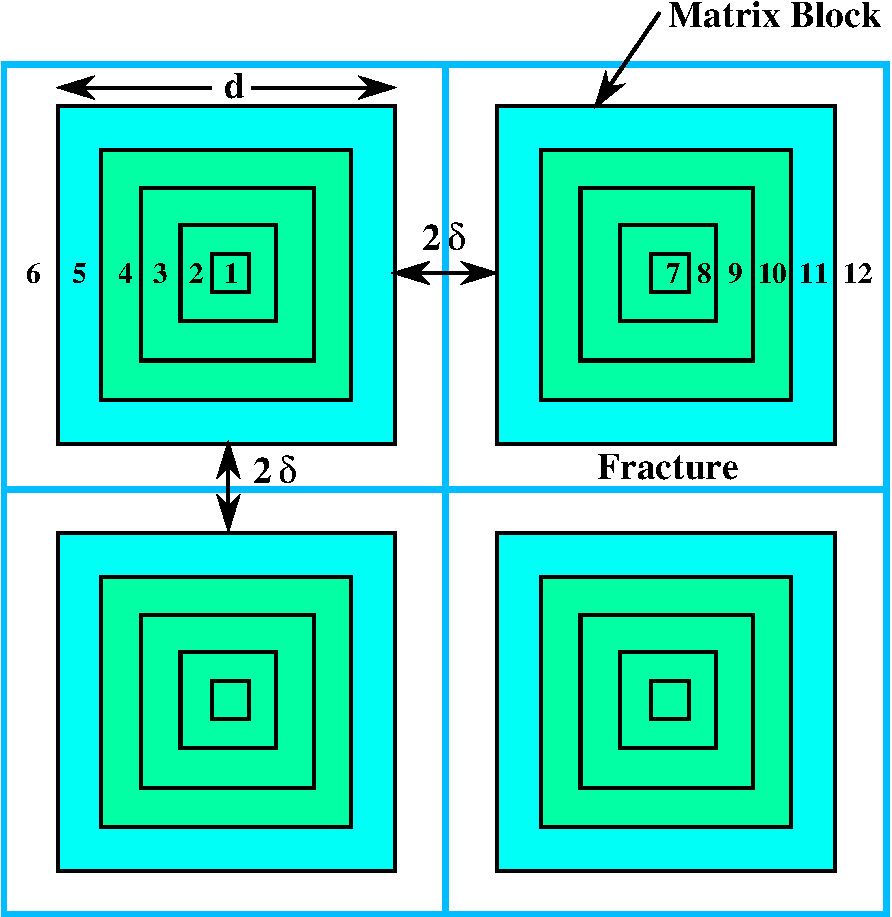
\includegraphics[scale=0.5]{./figs/mincl}
\parbox{4in}{\caption{Control volumes in DCDM multiple continuum model with fracture aperture $2\delta$ and matrix block size $d$.}\label{fminc}}
\end{figure}

Thermal conductivity at the interface between two control volumes is calculated using the harmonic average
\EQ
\kappa_{ll'} \eq \frac{\kappa_l \kappa_{l'}(d_l+d_{l'})}{d_l \kappa_{l'}+d_{l'}\kappa_l}.
\EN

The fracture volume $v_n$ is related to the REV volume $V_n$ by
\EQ
\epsilon \eq \frac{v_n}{V_n}.
\EN
According to the geometry in Figure~\ref{fminc} assuming a 3D orthogonal set of fractures,
\EQ
V_n \eq (d+2\delta)^3,
\EN
and
\EQ
v_n \eq (d+2\delta)^3 - d^3,
\EN
giving
\begin{subequations}
\BA
\epsilon &\eq 1-\frac{d^3}{(d+2\delta)^3} \eq 1-\left(\dfrac{1}{1+\dfrac{2\delta}{d}}\right)^3,\\
& ~\simeq~ \frac{6\delta}{d}.
\EA
\end{subequations}
The fracture aperture $2\delta$ is found to be in terms of $\epsilon$ and $d$
\EQ
2\delta \eq d \left(\frac{1}{(1-\epsilon)^{1/3}} -1\right).
\EN
A list of different sub-continua geometries and parameters implemented in PFLOTRAN is given in Table~\ref{tdcdmgeom}. Different independent and dependent parameters for the nested cube geometry are listed in Table~\ref{tnestedcube}.
The interfacial area $A_{nn'}^\a$ between fracture control volumes is equal to $\Delta y \Delta z$,  $\Delta z \Delta x$, $\Delta x \Delta y$ for $x$, $y$, and $z$ directions, respectively. 

In the case of nested cubes there are four possible parameters $(\epsilon, \, 2\delta, \, l_m,\, l_f)$, where $l_m$ denotes the matrix block size and $l_f$ refers to the fracture spacing, two of which are independent.

The fracture-matrix interfacial area $A_{nM}$ per unit volume is equal to
\EQ
A_{nM}^\b \eq \frac{\N_\b}{V} A_\b^0,
\EN
where the number density $\N_\b/V$ of secondary continua of type $\b$ is equal to
\EQ
\frac{\N_\b}{V} \eq \frac{1}{V} \frac{V_\b}{V_\b^0} \eq \frac{\epsilon_\b}{V_\b^0},
\EN
and $A_\b^0$ and $V_\b^0$ refer to the area and volume of each geometric type as listed in Table~\ref{tdcdm}.
\begin{table}\centering
\caption{DCDM geometric parameters.}\label{tdcdmgeom}
\vspace{3mm}
\begin{tabular}{lcc}
\toprule
Geometry & Area $A_\b^0$ & Volume $V_\b^0$\\
\midrule
Slab & $A$ & $A l$ \\
Nested Cubes & $6d^2$ & $d^3$\\
Nested Spheres & $4 \pi R^2$ & $\frac{4}{3}\pi R^3$\\
\bottomrule
\end{tabular}
\end{table}
The primary-secondary coupling term can then be written in the form
\EQ
\sum_\b\frac{\kappa_{nM}^{\a\b}}{d_n+d_{M}}\big(T_n^\a-T_{M}^\b\big) A_{nM}^\b \eq V_n
\sum_\b\frac{\epsilon_\b\kappa_{nM}^{\a\b}}{d_n+d_{M}}\big(T_n^\a-T_{M}^\b\big) \frac{A_\b^0}{V_\b^0}.
\EN

\begin{table}\centering
\caption{Independent and dependent nested cube parameters.}
\label{tnestedcube}
\vspace{3mm}
\begin{tabular}{lccc}
\toprule
\multicolumn{2}{c}{Independent} & \multicolumn{2}{c}{Dependent}\\
\midrule
$\epsilon$ & $l_f$ & $2\delta = l_f - l_m$ & $l_m = l_f(1-\epsilon)^{1/3}$\\
$\epsilon$ & $l_m$ & $2\delta = l_f - l_m$ & $l_f = l_m(1-\epsilon)^{-1/3}$\\
$2\delta$ & $l_f$ & $\epsilon = 1-(l_m/l_f)^3$ & $l_m = l_f - 2\delta$\\
$2\delta$ & $l_m$ & $\epsilon = 1-(l_m/_f)^3$ & $l_f = l_m + 2\delta$\\
$2\delta$ & $\epsilon$ & $l_m = 2\delta \Big(\dfrac{1}{(1-\epsilon)^{1/3}}-1\Big)^{-1}$ & $l_m = l-2\delta$\\
\bottomrule
\end{tabular}
\end{table}

In terms of partial differential equations the heat conservation equations may be written as
\begin{subequations}
\EQ
\frac{\p}{\p t} \epsilon \Big[\varphi \sum_\a s_\a \rho_\a U_\a + (1-\varphi) \rho_r C_r T_f\Big] + \bnabla\cdot \Big(\sum_\a \bq_\a \rho_\a H_\a -
%\epsilon
\kappa_f\bnabla T_f\Big) \eq -A_{fm} \kappa_{fm}\frac{\p T_m}{\p n},
\EN
and
\EQ
\frac{\p}{\p t} \rho_r C_r T_m + \frac{\p}{\p\xi} \Big(-\kappa_m\frac{\p T_m}{\p\xi}\Big) \eq 0,
\EN
for fracture and matrix temperatures $T_f$ and $T_m$, respectively, where $\xi$ represents the matrix coordinate assumed to be an effective 1D domain. The boundary condition 
\EQ
T_m(\xi_d,\,t\,|\,\br) \eq T_f(\br,\,t),
\EN
\end{subequations}
between fracture and matrix continua is imposed, where $\xi_d$ denotes the outer boundary of the matrix.

%The fracture thermal conductivity is defined as
%\EQ
%\kappa_f \eq \epsilon^{-1}\kappa.
%\EN

\subsection{Mode: Reactive Transport (Keyword {\tt CHEMISTRY})}\label{sec:chem}

The governing mass conservation equations for the geochemical transport mode for a multiphase system written in terms of a set of independent aqueous primary or basis species with the form
\EQ\label{rteqn}
\frac{\p}{\p t}\big(\varphi \sum_\a s_\a \Psi_j^\a\big) +
\nabla\cdot\sum_\a\bOmega_j^\a 
\eq Q_j - \sum_m\nu_{jm} I_m -\frac{\p S_j}{\p t},
\EN
and
\EQ
\frac{\p\varphi_m}{\p t} \eq \overline V_m I_m,
\EN
for minerals with molar volume $\overline V_m$, mineral reaction rate $I_m$ and mineral volume fraction $\varphi_m$ referenced to an REV. 
Sums over $\a$ in Eqn.\eqref{rteqn} are over all fluid phases in the system. The quantity $\Psi_j^\a$ denotes the total concentration of the $j$th primary species $\A_j^{\rm pri}$ in the $\a$th fluid phase defined by
\EQ
\Psi_j^\a = \delta_{l\a}^{} C_j^l + \sum_{i=1}^{N_{\rm sec}}\nu_{ji}^{\a} C_i^\a.
\EN
In this equation the subscript $l$ represents the aqueous electrolyte phase from which the primary species are chosen. The secondary species concentrations $C_i^\a$ are obtained from mass action equations corresponding to equilibrium conditions of the reactions
\EQ
\sum_j\nu_{ji}^\a\A_j^l \arrows \A_i^\a,
\EN
yielding
\EQ
C_i^\a \eq \frac{K_i^\a}{\gamma_i^\a} \prod_j \Big(\gamma_j^l C_j^l\Big)^{\nu_{ji}^\a},
\EN
with equilibrium constant $K_i^\a$, and activity coefficients $\gamma_k^\a$.
The total flux $\bOmega_j^\a$ for species-independent diffusion is given by
\EQ
\bOmega_j^\a \eq \big(\bq_\a - \varphi s_\a \bD_\a\bnabla\big)\Psi_j^\a.
\EN
The diffusion/dispersion coefficient $\bD_\a$ may be different for different phases, e.g. an aqueous electrolyte solution or gas phase, but is assumed to be species independent. Dispersivity currently must be described through a diagonal dispersion tensor. The Darcy velocity $\bq_\a$ for phase $\a$ is given by
\EQ
\bq_a \eq -\frac{kk_\a}{\mu_\a} \bnabla \big(p_\a -\rho_\a g z\big),
\EN
with bulk permeability of the porous medium $k$ and relative permeability $k_\a$, fluid viscosity $\mu_\a$, pressure $p_\a$, density $\rho_\a$, and acceleration of gravity $g$. The diffusivity/dispersivity tensor $\bD_\a$ is the sum of contributions from molecular diffusion and dispersion which for an isotropic medium has the form
\EQ
\bD_\a \eq %\varphi s 
%\Big(
\tau D_m + a_T \bI + \big(a_L-a_T\big)\frac{\bv\bv}{v},
%\Big),
\EN
with longitudinal and transverse dispersivity coefficients $a_L$, $a_T$, respectively, $\tau$ refers to tortuosity, and $D_m$ to the molecular diffusion coefficient. Currently, only longitudinal dispersion is implemented in PFLOTRAN.

The porosity may be calculated from the mineral volume fractions according to the relation
\EQ
\varphi \eq 1 - \sum_m \varphi_m. 
\EN

The temperature dependence of the diffusion coefficient is defined through the relation
\EQ
D_m(T) \eq D_m^\circ\exp\left[\frac{A_D}{R}\left(\frac{1}{T_0}-\frac{1}{T}\right)\right],
\EN
with diffusion activation energy $A_D$ in kJ/mol. The quantity $D_m^\circ$ denotes the diffusion coefficient at the reference temperature $T_0$ taken as 25\degc\ and the quantity $R$ denotes the gas constant ($8.317\times 10^{-3}$ kJ/mol/K).
The temperature $T$ is in Kelvin.

The quantity $Q_j$ denotes a source/sink term 
\EQ
Q_j \eq \sum_n\frac{q_M}{\rho}\Psi_j \delta(\br-\br_{n}),
\EN
where $q_M$ denotes a mass rate in units of kg/s, $\rho$ denotes the fluid density in kg/m$^3$, and $\br_{n}$ refers to the location of the $n$th source/sink. The quantity $S_j$ represents the sorbed concentration of the $j$th primary species considered in more detail in the next section.

Molality $m_i$ and molarity $C_i$ are related by the density of water $\rho_w$
\EQ
C_i \eq \rho_w m_i,
\EN
The activity of water is calculated from the approximate relation
\EQ
a_{\rm H_2O}^{} \eq 1 - 0.017 \sum_i m_i.
\EN

\subsubsection{Mineral Precipitation and Dissolution}

The reaction rate $I_m$ is based on transition state theory with the form
\EQ\label{Im}
I_m \eq -a_m\left(\sum_l k_{ml}(T) \P_{ml}\right) \Big(1-K_m Q_m\Big),
\EN
where the sum over $l$ represents contributions from parallel reaction mechanisms such as pH dependence etc., and where $K_m$ denotes the equilibrium constant, $a_m$ refers to the specific mineral surface area, and the ion activity product $Q_m$ is defined as
\EQ
Q_m \eq \prod_j \big(\gamma_j m_j\big)^{\nu_{jm}},
\EN
with molality $m_j$. The rate constant $k_{ml}$ is a function of temperature given by the Arrhenius relation
\EQ
k_{ml} (T) \eq k_{ml}^0 \exp\left[\frac{E_{ml}}{R}\Big(\frac{1}{T_0}-\frac{1}{T}\Big)\right],
\EN
where $k_{ml}^0$ refers to the rate constant at the reference temperature $T_0$ taken as 25\degc, with $T$ in units of Kelvin, $E_{ml}$ denotes the activation energy (kJ/mol),
and the quantity $\P_{ml}$ denotes the prefactor for the $l$th parallel reaction with the form
\EQ\label{prefactor}
\P_{ml} \eq \prod_i\dfrac{\big(\gamma_i m_i\big)^{\a_{il}^m}}{1+K_{ml}\big(\gamma_i m_i\big)^{\b_{il}^m} },
\EN
where the product index $i$ generally runs over both primary and secondary species, the quantities $\a_{il}^m$ and $\b_{il}^m$ refer to prefactor coefficients, and $K_{ml}$ is an attenuation factor.
The quantity $R$ denotes the gas constant ($8.317\times 10^{-3}$ kJ/mol/K). 

Porosity, permeability, tortuosity and mineral surface area may be updated optionally due to mineral precipitation and dissolution reactions according to the relations
\EQ\label{porosity}
\varphi \eq 1-\sum_m\varphi_m,
\EN
\EQ\label{permeability}
k \eq k_0 f(\varphi,\,\varphi_0,\,\varphi_c,\,a),
\EN
with
\BA
f &\eq \left(\frac{\varphi-\varphi_c}{\varphi_0-\varphi_c}\right)^a,\label{permf}\\
&\eq f_{\rm min} \ \ \ \text{if} \ \ \ \varphi \leq \varphi_c,\label{fmin}
\EA
\EQ\label{tortuosity}
\tau \eq \tau_0 \left(\frac{\varphi}{\varphi_0}\right)^b,
\EN
and
\EQ\label{surface_area_vf}
a_m \eq a_m^0 \left(\frac{\varphi_m}{\varphi_m^0}\right)^n  \left(\frac{1-\varphi}{1-\varphi_0}\right)^{n'},
\EN
where the super/subscript 0 denotes initial values, with a typical value for $n$ of $2/3$ reflecting the surface to volume ratio. Note that this relation only applies to primary minerals $(\varphi_m^0\ne 0)$. The quantity $\varphi_c$ refers to a critical porosity below which the permeability is assumed to be constant with scale factor $f_{\rm min}$.

In PFLOTRAN the solid is represented as an aggregate of minerals described quantitatively by specifying its porosity $\varphi$ and the volume fraction $\varphi_m$ of each primary mineral such that Eqn.\eqref{porosity} holds. Typically, however, the solid composition is specified by giving the mass fraction $y_m$ of each of the primary minerals making up the solid phase. The volume fraction is related to mole $x_m$ and mass $y_m$ fractions by the expressions
\begin{subequations}
\BA
\varphi_m &\eq (1-\varphi) \frac{x_m \overline V_m}{\sum_{m'} x_{m'} \overline V_{m'}},\\
&\eq (1-\varphi) \frac{y_m^{} \rho_m^{-1}}{\sum_{m'} y_{m'}^{} \rho_{m'}^{-1}},
\EA
\end{subequations}
where
\EQ
\rho_m^{} \eq W_m^{} \overline V_m^{-1}.
\EN
In these relations $W_m$ refers to the formula weight and $\overline V_m$ the molar volume of the $m$th mineral. The solid molar density $\eta_s$ is given by
\EQ
\eta_s \eq \frac{1}{\sum_m x_m \overline V_m},
\EN
which is related to the mass density $\rho_s$ by
\EQ
\rho_s \eq W \eta_s,
\EN
with the mean molecular weight $W$ equal to
\EQ
W \eq \sum_m x_m W_m \eq \frac{1}{\sum_m W_m^{-1} y_m^{}}.
\EN
Mass and mole fractions are related by the expression
\EQ
W_m x_m \eq W y_m.
\EN

\subsubsection{Sorption}

Sorption reactions incorporated into PFLOTRAN consist of ion exchange and surface complexation reactions for both equilibrium and multirate formulations.

\paragraph{Ion Exchange}

Ion exchange reactions may be represented either in terms of bulk- or mineral-specific rock properties.  Changes in bulk sorption properties can be expected as a result of mineral reactions.  However, only the mineral-based formulation enables these effects to be captured in the model.  The bulk rock sorption site concentration $\omega_\a$, in units of moles of sites per bulk sediment volume (mol/dm$^3$), is related to the bulk cation exchange capacity $Q_\a$ (mol/kg) by the expression
\EQ
\omega_\a \eq \frac{N_{\rm site}}{V} \eq \frac{N_{\rm site}}{M_s} \frac{M_s}{V_s} \frac{V_s}{V} \eq Q_\a \rho_s (1-\phi).
\EN
The cation exchange capacity associated with the $m$th mineral is defined on a molar basis as
\EQ
\omega_m^{\rm CEC} \eq \frac{N_m}{V} \eq \frac{N_m}{M_m} \frac{M_m}{V_m} \frac{V_m}{V} \eq Q_m^{\rm CEC} \rho_m \phi_m.
\EN

In PFLOTRAN ion exchange reactions are expressed in the form
\EQ\label{ex1}
z_i \A_j + z_j X_{z_i}^\a\A_i \arrows z_j \A_i + z_i X_{z_j}^\a\A_j,
\EN
with valencies $z_j$, $z_i$ of cations $\A_j$ and $\A_i$, respectively. The reference cation is denoted by $\A_j$ and $\A_i, \,i\!\ne\! j$ represents all other cations. 
The corresponding mass action equation is given by
\EQ\label{ionexmassact}
K_{ji}^\a \eq \frac{(k_j^\a)^{z_i}}{(k_i^\a)^{z_j}} \eq \left(\frac{X_j^\a}{a_j}\right)^{z_i} \left(\frac{a_i}{X_i^\a}\right)^{z_j}.
\EN
Using the Gaines-Thomas convention, the equivalent fractions $X_k^\a$ are defined by
\EQ
X_k^\a = \frac{z_k S_k^\a}{\displaystyle\sum_l z_l S_l^\a} = \frac{z_k}{\omega_\a}S_k^\a,
\EN
with 
\EQ
\sum_k X_k^\a = 1.
\EN
The site concentration $\omega_\a$ is defined by
\EQ
\omega_\a = \sum_k z_k S_k^\a,
\EN
where $\omega_\a$ is related to the cation exchange capacity $Q_\a$ (CEC) by the expression
\EQ
\omega_\a = (1-\varphi) \rho_s \, Q_\a,
\EN
with solid density $\rho_s$ and porosity $\varphi$. 

An alternative form of reactions \ref{ex1} often found in the literature is
\EQ\label{rxn2}
\frac{1}{z_j} \A_j + \frac{1}{z_i} X_{z_i}^\a\A_i \arrows \frac{1}{z_i} \A_i + \frac{1}{z_j} X_{z_j}^\a\A_j,
\EN
obtained by dividing reaction \ref{ex1} through by the product $z_i z_j$.  In addition the reaction may be written in reverse order.
The mass action equations corresponding to reactions \ref{rxn2} have the form
\EQ
{K'}_{ji}^\a \eq \frac{({k'}_j^\a)^{1/z_j}}{({k'}_i^\a)^{1/z_i}} \eq \left(\frac{X_j^\a}{a_j}\right)^{1/z_j} \left(\frac{a_i}{X_i^\a}\right)^{1/z_i}.
\EN
The selectivity coefficients corresponding to the two forms are related by the expression
\EQ
K_{ji}^\a \eq \left({K'}_{ji}^\a\right)^{z_i z_j},
\EN
and similarly for $k_i^\a$, $k_j^\a$. When comparing with other formulations it is important that the user determine which form of the ion exchange reactions are being used and make the appropriate transformations.

For equivalent exchange $(z_j\!=\!z_i\!=\!z)$, an explicit expression exists for the sorbed concentrations given by
\EQ
S_j^\a \eq \frac{\omega_\a}{z} \frac{k_j^\a \gamma_j m_j^{}}{\displaystyle\sum_l k_l^\a \gamma_l m_l^{}},
\EN
where $m_k$ denotes the $k$th cation molality. This expression follows directly from the mass action equations and conservation of exchange sites.

In the more general case $(z_i\ne z_j)$ it is necessary to solve the nonlinear equation
\EQ
X_j^\a + \sum_{i\ne j} X_i^\a \eq 1,
\EN
for the reference cation mole fraction $X_j$. 
From the mass action equation Eqn.\eqref{ionexmassact}
it follows that
\EQ
X_i^\a\eq k_i^\a a_i\left(\frac{X_j^\a}{k_j^\a a_j}\right)^{z_i/z_j}.
\EN
Defining the function
\EQ
f(X_j^\a) \eq X_j^\a + \sum_{i\ne j}X_i^\a(X_j^\a)-1,
\EN
its derivative is given by
\EQ
\frac{df}{dX_j^\a} \eq 1 - \frac{1}{z_jX_j^\a}\sum_{i\ne j} z_i k_i^\a a_i \left(\frac{X_j^\a}{k_j^\a a_j}\right)^{z_i/z_j}.
\EN
The reference mole fraction is then obtained by Newton-Raphson iteration
\EQ
(X_j^\a)^{k+1} \eq (X_j^\a)^k -\dfrac{f[(X_j^\a)^k]}{\dfrac{df[(X_j^\a)^k]}{dX_j^\a}}.
\EN

The sorbed concentration for the $j$th cation appearing in the accumulation term is given by
\EQ
S_j^\a \eq \frac{\omega_\a}{z_j} X_j^\a,
\EN
with the derivatives for $j\ne l$
\begin{subequations}
\BA
\dfrac{\p S_j^\a}{\p m_l} &\eq -\frac{\omega_\a}{m_l} \dfrac{X_j^\a X_l^\a}{\displaystyle\sum_l z_l X_l^\a},\\
&\eq -\frac{1}{m_l} \dfrac{z_jz_lS_j^\a S_l^\a}{\displaystyle\sum_l z_l^2 S_l^\a},
\EA
\end{subequations}
and for $j=l$
\begin{subequations}
\BA
\dfrac{\p S_j^\a}{\p m_j} &\eq \frac{\omega_\a X_j^\a}{z_j m_j} \left(1-\dfrac{z_j X_j^\a}{\displaystyle\sum_{l} z_{l} X_{l}^\a}\right),\\
&\eq \frac{S_j^\a}{m_j} \left(1-\dfrac{z_j^2 S_j^\a}{\displaystyle\sum_{l} z_{l}^2 S_{l}^\a}\right).
\EA
\end{subequations}

\paragraph{Surface Complexation}

Surface complexation reactions are assumed to have the form
\EQ\label{srfrxn}
\nu_\a >\!\!\chi_\a + \sum_j\nu_{ji} \A_j \arrows \!>\!\! \mcS_{i\a},
\EN
for the $i$th surface complex $>\!\!\mcS_{i\a}$ on site $\a$ and empty site $>\!\!\chi_\a$.
As follows from the corresponding mass action equation the equilibrium sorption concentration $S_{i\a}^{\rm eq}$ is given by
\EQ
S_{i\a}^{\rm eq}\eq \frac{\omega_\a K_i Q_i}{1+\sum_l K_lQ_l},
\EN
and the empty site concentration by
\EQ
S_\a^{\rm eq}\eq\frac{\omega_\a}{1+\sum_l K_lQ_l},
\EN
where the ion activity product $Q_i$ is defined by
\EQ
Q_i\eq\prod_j\big(\gamma_jC_j\big)^{\nu_{ji}}.
\EN
The site concentration $\omega_\a$ satisfies the relation
\EQ\label{totsite}
\omega_\a \eq S_\a + \sum_i S_{i\a},
\EN
and is constant.
The equilibrium sorbed concentration $S_{j\a}^{\rm eq}$ is defined as
\EQ\label{qeq}
S_{j\a}^{\rm eq} \eq \sum_i \nu_{ji}^{} S_{i\a}^{\rm eq}\eq \frac{\omega_\a}{1+\sum_l K_lQ_l} \sum_i \nu_{ji}K_i Q_i.
\EN

\paragraph{Multirate Sorption}

In the multirate model the rates of sorption reactions are described through a kinetic relation given by
\EQ\label{sorbed}
\frac{\p S_{i\a}}{\p t} \eq k_\a^{} \big(S_{i\a}^{\rm eq}-S_{i\a}\big),
\EN
for surface complexes, and
\BA\label{fsite}
\frac{\p S_{\a}}{\p t} &\eq -\sum_i k_\a^{} \big(S_{i\a}^{\rm eq}-S_{i\a}\big),\\
&\eq k_\a\big(S_\a^{\rm eq}-S_{\a}\big),
\EA
for empty sites, where $S_\a^{\rm eq}$ denotes the equilibrium sorbed concentration. For simplicity, in what follows it is assumed that $\nu_\a\!=\!1$. 
With each site $\a$ is associated a rate constant $k_\a$ and site concentration $\omega_\a$. These quantities are defined through a given distribution of sites $\wp(\a)$, such that
\EQ
\int_0^\infty \wp(k_\a)dk_\a \eq 1.
\EN
The fraction of sites $f_\a$ belonging to site $\a$ is determined from the relation
\EQ
f_\a \eq \int_{k_\a-\Delta k_\a/2}^{k_\a+\Delta k_\a/2} \wp(k_\a)dk_\a \simeq \wp(k_\a)\Delta k_\a,
\EN
with the property that
\EQ
\sum_\a f_\a =1.
\EN
Given that the total site concentration is $\omega$, then the site concentration $\omega_\a$ associated with site $\a$ is equal to
\EQ
\omega_\a \eq f_\a \omega.
\EN

An alternative form of these equations is obtained by introducing the total sorbed concentration for the $j$th primary species for each site defined as
\EQ
S_{j\a}\eq\sum_i \nu_{ji}S_{i\a}.
\EN
Then the transport equations become
\EQ\label{totj}
\frac{\p}{\p t}\left(\varphi \Psi_j + \sum_{\a}S_{j\a}\right) + \bnabla\cdot\bOmega_j \eq  - \sum_m\nu_{jm}I_m.
\EN
The total sorbed concentrations are obtained from the equations
\EQ\label{sja}
\frac{\p S_{j\a}}{\p t} \eq k_\a^{} \big(S_{j\a}^{\rm eq}-S_{j\a}\big).
\EN

\subsubsection{Sorption Isotherm}

A sorption isotherm $S_j$ may be specified for any primary species $\A_j$. 
The following transport equation is solved 
\EQ
\frac{\p}{\p t} \varphi s C_j + \bnabla\cdot\bF_j \eq -\frac{\p S_j}{\p t},
\EN
with $C_j \eq \rho_w m_j$ and $\rho_w$ refers to the density of pure water.
Three distinct models are available for the sorption isotherm $S_j$:
\begin{itemize}
\item linear $K_D$ model
\EQ\label{linkd}
S_j \eq K_j^D \gamma_j m_j,
\EN
with activity coefficient $\gamma_j$ and molality $m_j$,
\item Langmuir isotherm:
\EQ\label{Langmuir}
S_j \eq \frac{K_j^L b_j^L \gamma_j m_j}{(1+K_j^L \gamma_j m_j)},
\EN
with Langmuir coefficients $K_j^L$ and $b_j^L$, and
\item Freundlich isotherm:
\EQ\label{Freundlich}
S_j \eq K_j^F \big(\gamma_j m_j\big)^{(1/n_j^F)},
\EN
with coefficients $K_j^F$ and $n_j^F$.
\end{itemize}
The linear $K_D$ model results in the retardation factor $\R_j$ given by
\EQ
\R_j \eq 1 + \frac{\gamma_j K_j^D}{\varphi s \rho_w}.
\EN
In terms of the retardation the transport equation becomes
\EQ
\frac{\p}{\p t} \big(\R_j\varphi s \rho_w m_j\big) + \bnabla\cdot\bF_j \eq 0.
\EN

\subsubsection{Colloid-Facilitated Transport}

Colloid-facilitated transport is implemented into PFLOTRAN based on surface complexation reactions. Competition between mobile and immobile colloids and stationary mineral surfaces is taken into account. Colloid filtration processes are not currently implemented into PFLOTRAN. 
A colloid is treated as a solid particle suspended in solution or attached to a mineral surface. Colloids may be generated through nucleation of minerals in solution, although this effect is not included currently in the code.

Three separate reactions may take place involving competition between mobile and immobile colloids and mineral surfaces
\BA
>\!X_k^\m + \sum_j\nu_{jk}\A_j &\arrows >\!S_k^\m,\\
>\!X_k^\im + \sum_j\nu_{jk}\A_j &\arrows >\!S_k^\im,\\
>\!X_k^s + \sum_j\nu_{jk}\A_j &\arrows >\!S_k^s,
\EA
with corresponding reaction rates $I_k^\m$, $I_k^\im$, and $I_k^s$, where the superscripts $s$, $m$, and $im$ denote mineral surfaces, and mobile and immobile colloids, respectively. In addition, reaction with minerals $\M_s$ may occur according to the reaction
\EQ
\sum_j\nu_{js}\A_j \arrows \M_s.
\EN
The transport equations for primary species, mobile and immobile colloids, read
\BA
\frac{\p}{\p t} \varphi s_l \Psi_j^l + \bnabla\cdot\bOmega_j^l &\eq -\sum_k\nu_{jk}\big(I_k^\m + I_k^\im + \sum_s I_k^s\big) - \sum_s \nu_{js} I_s,\label{rateform}\\
\frac{\p}{\p t} \varphi s_l S_k^\m + \bnabla\cdot\bq_c S_k^\m & \eq I_k^\m,\label{mobile}\\
\frac{\p}{\p t} S_k^\im & \eq I_k^\im,\label{immobile}\\
\frac{\p}{\p t} S_k^s & \eq I_k^s,\label{solid}
\EA
where $\bq_c$ denotes the colloid Darcy velocity which may be greater than the fluid velocity $\bq$.
For conditions of local equilibrium the sorption reaction rates may be eliminated and replaced by algebraic sorption isotherms to yield
\EQ\label{eqform}
\frac{\p}{\p t}\Big[ \varphi s_l \Psi_j^l + \sum_k \nu_{jk} \big(\varphi s_l S_k^\m + S_k^\im + \sum_s S_k^s\big) \Big] + \bnabla\cdot\Big(\bOmega_j^l + \bq_c \sum_k \nu_{jk} S_k^\m\Big) \eq - \sum_s \nu_{js} I_s.
\EN

In the kinetic case either form of the primary species transport equations given by Eqn.\eqref{rateform} or \eqref{eqform} can be used provided it is coupled with the appropriate kinetic equations Eqns.\eqref{mobile}--\eqref{solid}. The mobile case leads to additional equations that must be solved simultaneously with the primary species equations. A typical expression for $I_k^m$ might be
\EQ
I_k^m \eq k_k\big(S_k^m - S_{km}^{\rm eq}\big),
\EN
with rate constant $k_k$ and where $S_{km}^{\rm eq}$ is a known function of the solute concentrations. In this case, Eqn.\eqref{mobile} must be added to the primary species transport equations. Further reduction of the transport equations for the case where a flux term is present in the kinetic equation is not possible in general for complex flux terms.

\subsection{Tracer Mean Age}

PFLOTRAN implements the Eulerian formulation of solute age for a nonreactive tracer following Goode (1996). PFLOTRAN solves the advection-diffusion/dispersion equation for the mean age given by
\EQ
\frac{\p}{\p t} \varphi s AC + \bnabla\cdot\Big(\bq AC - \varphi s D \bnabla (AC)\Big) \eq \varphi s C,
\EN
where $A$ denotes the mean age of the tracer with concentration $C$. Other quantities appearing in the age equation are identical to the tracer transport equation for a partially saturated porous medium with saturation state $s$. The age and tracer transport equations are solved simultaneously for the age-concentration $\alpha = A C$ and tracer concentration $C$. The age-concentration $\a$ satisfies the usual advection-diffusion-dispersion equation with a source term on the right-hand side.

The mean tracer is calculated in PFLOTRAN by adding the species {\tt Tracer\_Age} together with {\tt Tracer} to the list of primary species
%\newpage
\begin{verbatim}
  PRIMARY_SPECIES
    Tracer
    Tracer_Age
  /
\end{verbatim}
including sorption through a constant $K_d$ model if desired
\begin{verbatim}
  SORPTION
    ISOTHERM_REACTIONS
      Tracer
        TYPE LINEAR 
        DISTRIBUTION_COEFFICIENT 500. ! kg water/m^3 bulk
      /
      Tracer_Age
        TYPE LINEAR 
        DISTRIBUTION_COEFFICIENT 500. ! kg water/m^3 bulk
      /
    /
  /
\end{verbatim}
and specifying these species in the initial and boundary {\tt CONSTRAINT} condition as e.g.:
\begin{verbatim}
CONSTRAINT initial
  CONCENTRATIONS
    Tracer     1.e-8        F
    Tracer_Age 1.e-16       F
  /
/
\end{verbatim}
Output is given in terms of $\alpha$ and $C$ from which the mean age $A$ can be obtained as $A\eq\alpha/C$. 

\subsection{Thermodynamic Database}

PFLOTRAN reads thermodynamic data from a database that may be customized by the user. Reactions included in the database consist of aqueous complexation, mineral precipitation and dissolution, gaseous reactions, and surface complexation. Ion exchange reactions and their selectivity coefficients are entered directly from the input file. 
A standard database supplied with the code is referred to as {\tt hanford.dat} and is found in the {\tt ./database} directory in the PFLOTRAN mercurial repository. This database is an ascii text file that can be edited by any editor and is equivalent to the EQ3/6 database:
\begin{verbatim}
data0.com.V8.R6
CII: GEMBOCHS.V2-EQ8-data0.com.V8.R6
THERMODYNAMIC DATABASE
generated by GEMBOCHS.V2-Jewel.src.R5 03-dec-1996 14:19:25
\end{verbatim}
The database provides equilibrium constants in the form of log $K$ values at a specified set of temperatures listed in the top line of the database. A least squares fit is used to interpolate the log $K$ values between the database temperatures using a Maier-Kelly expansion of the form
\EQ\label{mk}
\log K \eq c_{-1} \ln T + c_0 + c_1 T + \frac{c_2}{T} + \frac{c_3}{T^2},
\EN
with fit coefficients $c_i$. 
The thermodynamic database stores all chemical reaction properties (equilibrium constant $\log K_r$, reaction stoichiometry $\nu_{ir}$, species valence $z_i$, Debye parameter $a_i$, mineral molar volume $\overline V_m$, and formula weight $w_i$) used in PFLOTRAN. The database is divided into 5 blocks as listed in Table~\ref{tdatabase}, consisting of
database primary species, aqueous complex reactions, gaseous reactions, mineral reactions, and surface complexation reactions. 
Each block is terminated by a line beginning with {\tt 'null'}. 
The quantity $N_{\rm temp}$ refers to the number of temperatures at which log $K$ values are stored in the database.
In the {\tt hanford.dat} database $N_{\rm temp}=8$ with equilibrium constants stored at the temperatures: 0, 25, 60, 100, 150, 200, 250, and 300\degc. The pressure is assumed to lie along the saturation curve of pure water for temperatures above 25\degc\ and is equal to 1 bar at lower temperatures.
Reactions in the database are assumed to be written in the canonical form
\EQ
\A_r \arrows \sum_{i=1}^{\rm nspec} \nu_{ir}\A_i,
\EN
for species $\A_r$, where {\tt nspec} refers to the number of aqueous or gaseous species $\A_i$ on the right-hand side of the reaction. 
Redox reactions in the standard database {\tt hanford.dat} are usually written in terms of O$_{2(g)}$.
Complexation reactions involving redox sensitive species are written in such a manner as to preserve the redox state.


\begin{table}[h]\centering
\caption{Format of thermodynamic database.}\label{tdatabase}
\vspace{3mm}
%\footnotesize
\begin{tabular}{ll}
\hline
Primary Species: & name, $a_0$, $z$, $w$\\
Secondary Species: & name, nspec, ($\nu$(n), name($n$), $n$=1, nspec), log$K$(1:$N_{\rm temp}$), $a_0$, $z$, $w$\\
Gaseous Species: & name, $\overline V$, nspec, ($\nu$(n), name($n$), $n$=1, nspec), log$K$(1:$N_{\rm temp}$), $w$ \\
Minerals: & name, $\overline V$, nspec, ($\nu$(n), name($n$), $n$=1, nspec), log$K$(1:$N_{\rm temp}$), $w$\\
Surface Complexes: & $>$name, nspec, $\nu$, $>$site, 
($\nu$(n), name($n$), $n$=1, nspec-1), \\
&\hspace{3in} log$K$(1:$N_{\rm temp}$), $z$, $w$\\
\hline
\end{tabular}
\end{table}

\section{Method of Solution}

\setcounter{equation}{0}

The flow and heat equations (Modes: RICHARDS, MPHASE, FLASH2, THC, \ldots) are solved using a fully implicit backward Euler approach based on Newton-Krylov iteration.
Both fully implicit backward Euler and operator splitting solution methods are supported for reactive transport.

\subsection{Fully Implicit}

In a fully implicit formulation the nonlinear equations for the residual function $\bR$ given by
\EQ
\bR(\bx) \eq \bzero,
\EN
are solved using an iterative solver based on the Newton-Raphson equations
\EQ
\bJ^{(i)} \delta\bx^{(i+1)} \eq -\bR^{(i)},
\EN
at the $i$th iteration. Iteration stops when
\EQ
\left|\bR^{(i+1)}\right| < \epsilon,
\EN
or if
\EQ
\big|\delta\bx^{(i+1)}\big| < \delta.
\EN
However, the latter criteria does not necessarily guarantee that the residual equations are satisfied.
The solution is updated from the relation
\EQ
\bx^{(i+1)} \eq \bx^{(i)} + \delta\bx^{(i+1)}.
\EN
For the logarithm of the concentration with $\bx=\ln\by$,
the solution is updated according to the equation
\EQ
\by^{(i+1)} \eq \by^{(i)} {\rm e}^{\delta\ln\by^{(i+1)}}.
\EN

\subsubsection{Multirate Sorption}

The residual function incorporating the multirate sorption model can be further simplified by solving analytically the finite difference form of kinetic sorption equations. This is possible when these equations are linear in the sorbed concentration $S_{j\a}$ and because they do not contain a flux term. Thus discretizing Eqn.\eqref{sja} in time using the fully implicit backward Euler method gives
\EQ
\frac{S_{j\a}^{t+\Delta t}-S_{j\a}^t}{\Delta t} \eq k_\a \big(f_\a S_{j\a}^{\rm eq} - S_{j\a}^{t+\Delta t}\big).
\EN
Solving for $S_{j\a}^{t+\Delta t}$ yields
\EQ\label{sjadt}
S_{j\a}^{t+\Delta t} \eq \frac{S_{j\a}^t + k_\a \Delta t f_\a S_j^{\rm eq}}{1+k_\a\Delta t}.
\EN
From this expression the reaction rate can be calculated as
\EQ
\frac{S_{j\a}^{t+\Delta t}-S_{j\a}^t}{\Delta t} \eq \frac{k_\a}{1+k_\a\Delta t} \big(f_\a S_{j\a}^{\rm eq} - S_{j\a}^t\big).
\EN
The right-hand side of this equation is a known function of the solute concentration and thus by substituting into Eqn.\eqref{totj} eliminates the appearance of the unknown sorbed concentration. Once the transport equations are solved over a time step, the sorbed concentrations can be computed from Eqn.\eqref{sjadt}.

\subsection{Operator Splitting}

Operator splitting involves splitting the reactive transport equations into a nonreactive part and a part incorporating reactions. This is accomplished by writing Eqns.\eqref{rteqn} as the two coupled equations
\EQ
\frac{\p}{\p t}\big(\varphi \sum_\a s_\a \Psi_j^\a\big) +
\nabla\cdot\sum_\a\big(\bq_\a - \varphi s_\a \bD_\a\bnabla\big)\Psi_j^\a \eq Q_j,
\EN
and
\EQ
\frac{d}{d t}\big(\varphi \sum_\a s_\a \Psi_j^\a\big) \eq - \sum_m\nu_{jm} I_m -\frac{\p S_j}{\p t},
\EN
The first set of equations are linear in $\Psi_j$ (for species-independent diffusion coeffients) and solved over over a time step $\Delta t$ resulting in $\Psi_j^*$. The result for $\Psi_j^*$ is inverted to give the concentrations $C_j^*$ by solving the equations
\EQ
\Psi_j^* \eq C_j^* + \sum_i \nu_{ji} C_i^*,
\EN
where the secondary species concentrations $C_i^*$ are nonlinear functions of the primary species concentrations $C_j^*$. With this result the second set of equations are solved implicitly for $C_j$ at $t+\Delta t$ using $\Psi_j^*$ for the starting value at time $t$.

\subsubsection{Constant $K_d$}

As a simple example of operator splitting consider a single component system with retardation described by a constant $K_d$. According to this model the sorbed concentration $S$ is related to the aqueous concentration by the linear equation
\EQ\label{skd}
S \eq K_d C.
\EN
The governing equation is given by
\EQ
\frac{\p}{\p t} \varphi C + \bnabla\cdot\big(\bq C -\varphi D \bnabla C\big) \eq -\frac{\p S}{\p t}.
\EN
If $C(x,\,t;\, \bq,\,D)$ is the solution to the case with no retardation (i.e. $K_d=0$), then $C(x,\,t;\, \bq/R,\,D/R)$ is the solution with retardation $(K_d>0)$,
with
\EQ
R = 1+\frac{1}{\varphi}K_d.
\EN
Thus propagation of a front is retarded by the retardation factor $R$.

In operator splitting form this equation becomes
\EQ
\frac{\p}{\p t} \varphi C + \bnabla\cdot\big(\bq C -\varphi D \bnabla C\big) \eq 0,
\EN
and
\EQ
\frac{d}{d t} \varphi C \eq -\frac{d S}{d t}.
\EN
The solution to the latter equation is given by
\EQ
\varphi C^{t+\Delta t} - \varphi C^* \eq -\big(S^{t+\Delta t} - S^t\big),
\EN
where $C^*$ is the solution to the nonreactive transport equation. Using Eqn.\eqref{skd}, this result can be written as
\EQ
C^{t+\Delta t} \eq \frac{1}{R} C^* + \left(1-\frac{1}{R}\right) C^t.
\EN
Thus for $R=1$, $C^{t+\Delta t}=C^*$ and the solution advances unretarded. As $R\rightarrow\infty$, $C^{t+\Delta t} \rightarrow C^t$ and the front is fully retarded.

\newpage

\section{Code Structure}

\setcounter{equation}{0}

A flow diagram of the PFLOTRAN code structure is shown in Figure~\ref{fdiag}.

\begin{figure}[h]\centering
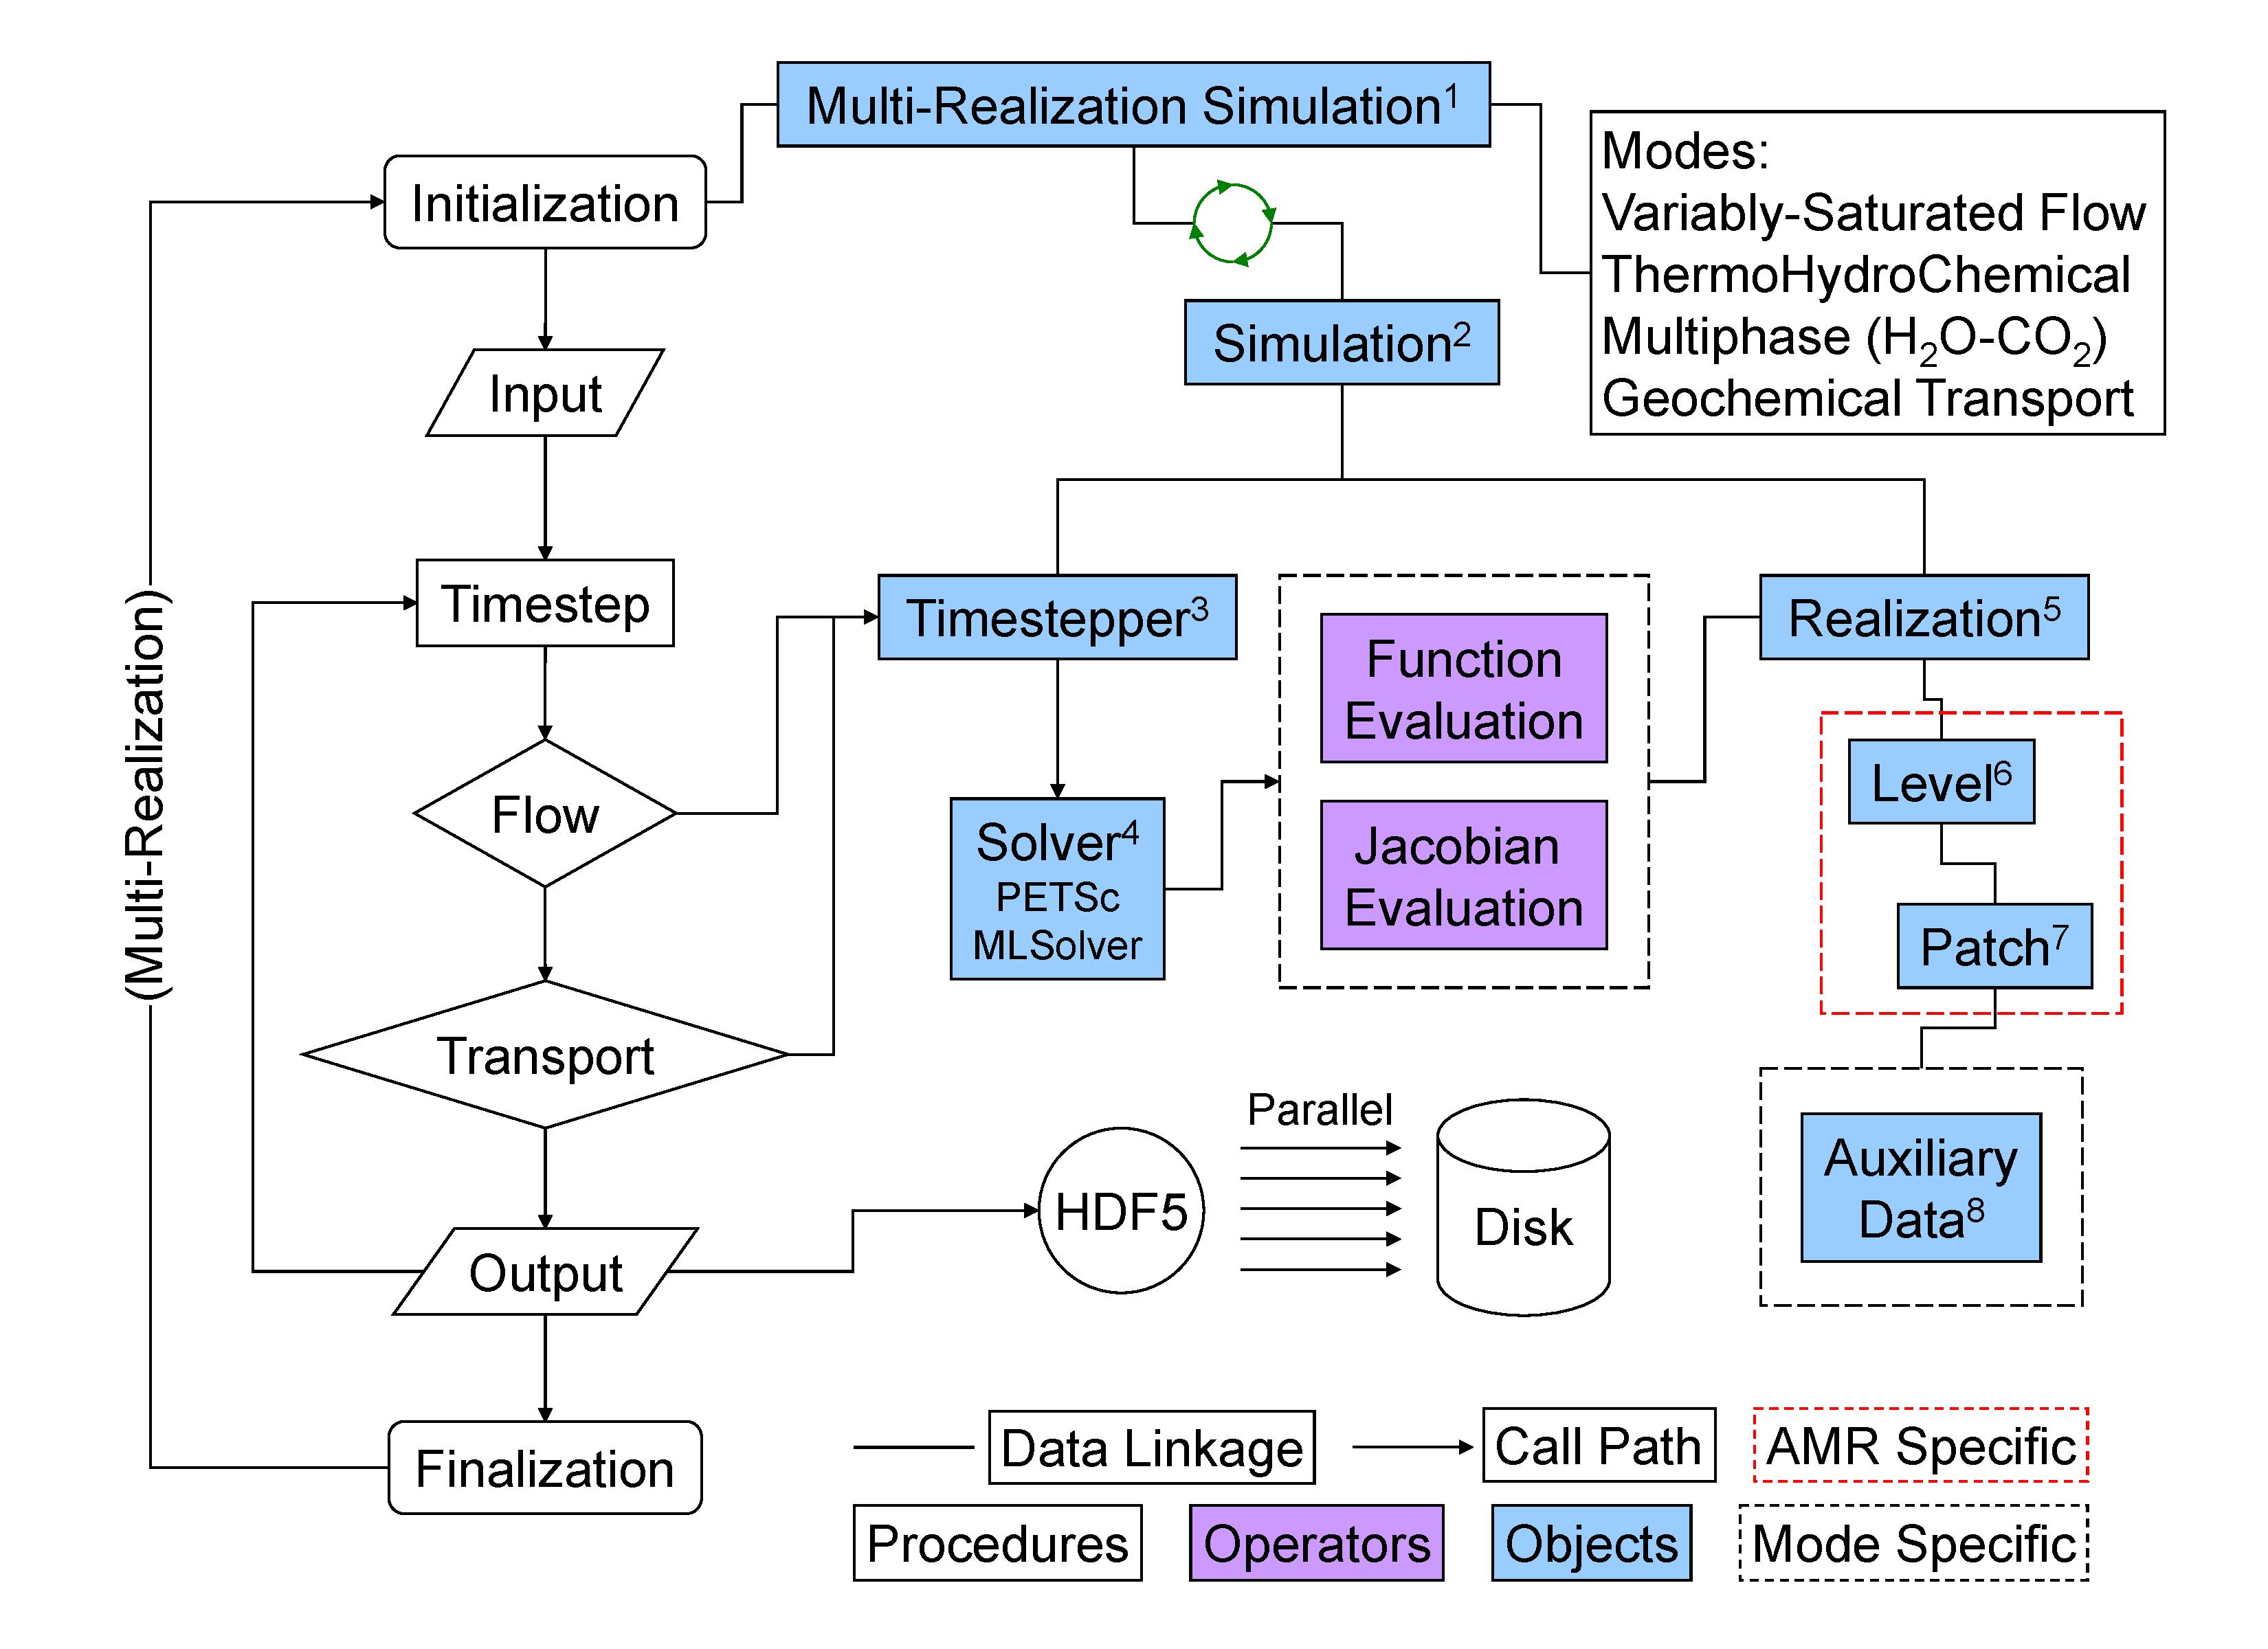
\includegraphics[scale=0.3]{./figs/multi-realization_flowchart}
\caption{Flow diagram of PFLOTRAN illustrating use of procedures, operators, and objects.}\label{fdiag}
\end{figure}

Flow diagram definitions:
\begin{enumerate}
\item {\bf Multi-Realization Simulation} object: Highest level data structure providing all information for running simulations composed of multiple realizations
\item {\bf Simulation} object: Data structure providing all information for running a single simulation
\item {\bf Timestepper} object: Pointer to Newton-Krylov solver and tolerances associated with time stepping
\item {\bf Solver} object: Pointer to nonlinear Newton and linear Krylov solvers (PETSc) along with associated convergence criteria
\item {\bf Realization} object: Pointer to all discretization and field variables associated with a single realization of a simulation
\item {\bf Level} object: Pointer to discretization and field variables associated with a single level of grid refinement within a realization
\item {\bf Patch} object: Pointer to discretization and field variables associated with a subset of grid cells within a level
\item {\bf Auxiliary Data} object: Pointer to auxiliary data within a realization/patch
\end{enumerate}


In order to facilitate code development and better preserve the extensibility and modularity of the code, an object-oriented coding paradigm is employed within PFLOTRAN.  In comparison to traditional procedural paradigms, the object-oriented programming paradigm facilitates code modification and reuse.  Within the context of PFLOTRAN, the utilization of this paradigm greatly accelerates the incorporation of new flow and transport modes through the extension of existing algorithms.  The compartmentalization of methods, processes and data enables the spawning of multi-realization simulations, each of which can be simultaneously run in parallel (i.e. each realization of the multi-realization simulation can be run in parallel utilizing multiple processor cores).

\newpage

\section{PFLOTRAN regression test manager}

The test manager for PFLOTRAN is a python program that is responsible
for reading a configuration file, identifying the tests declared in
the file, running PFLOTRAN on the appropriate input files, and then
comparing the results to a known "gold standard" output file.

\subsection{Running the test manager}
The test manager can be run in two ways, either as part of the build
system using ``make'' or manually.

There are two options for calling the test manager through make,
``make check'' and ``make test''. The ``check'' target runs a set of
tests that verify that PFLOTRAN is built and running correctly on a
given system. This would be run by user to verify that their
installation of PFLOTRAN is working. The ``test'' target runs a fuller
set of regression tests intended to identify when changes to the code
cause significant changes to PFLOTRAN's results.

Calling the test manager through make relies on make variables from
PETSc to determine the correct version of python to use, if PFLOTRAN
was build with MPI, and optional configurations such as unstructured
meshes. The version of python used to call the test manager can be
changed from the command line by specifying python:

\begin{verbatim}
$ make PYTHON=/opt/local/bin/python3.3 check
\end{verbatim}

The test manager produces terse output by default, only reporting the
test name whether it passed or failed. Verbose output reports the
reason why a test failed, the call to PFLOTRAN, and ``diff'' command:

\begin{verbatim}
$ make VERBOSE=true check
\end{verbatim}

To call the test manager manually:
\begin{verbatim}
$ cd pflotran/test
$ python regression-tests.py --executable ../src/pflotran/pflotran \
    --config-file shortcourse/copper_leaching/cu_leaching.cfg \
    --tests cu_leaching --verbose
\end{verbatim}

Some important command line arguments when running manually are:
\begin{itemize}
\item executable : the path to the PFLOTRAN executable
\item mpiexec : the name of the executable for launching parallel
  jobs, (mpiexec, mpirun, aprun, etc).
\item config-file : the path to the configuration file containing the
  tests you want to run
\item recursive-search : the path to a directory. The test manager
  searches the directory and all its sub-directories for configuration
  files.
\item tests : a list of test names that should be run
\item suites : a list of test suites that should be run
\item verbose : verbose output, includes the command to run PFLOTRAN,
  the command to diff results, and details about why a test failed.
\item update : indicate that the the gold standard test file for a
  given test should be updated to the current output.
\item new-tests : indicate that the test is new and current output
  should be used for gold standard test file.
\end{itemize}

The full list of command line options and a brief description can be
found by running with the ``--help'' flag:
\begin{verbatim}
$ python regression-tests.py --help
\end{verbatim}

\subsection{Configuration Files}
The configuration files are in standard ``cfg'' or windows ``ini''
file format. They consist of a series of sections with key-value pairs:
\begin{verbatim}
[section-name]
key = value
\end{verbatim}
Section names should be all lower case, and spaces must be replaced by
a hyphen or underscore.

A test is declared as a section in the configuration file. It is assumed that
there will be a PFLOTRAN input file with the same name as the test
section. The key-value pairs in a test section define how the test is
run and the output is compared to the gold standard file. 
\begin{verbatim}
[calcite-kinetics]
#look for an input file named `calcite-kinetics.in'
np = 2
timeout = 30.0
concentration = 1.0e-10 absolute
\end{verbatim}

\begin{itemize}
\item np = N, (optional), indicates a parallel test run with N processors. Default is serial.
\item timeout = N, (optional), indicates that the test should be allowed to run
  for N seconds before it is killed. Default is 60.0 seconds.
\item TYPE = TOLERANCE COMPARISON, indicates that data in the
  regression file of type TYPE should be compared using a tolerance of
  TOLERANCE. Know data types are listed below.
\end{itemize}

The data types and default tolerances are:
\begin{itemize}
\item time = 5 percent
\item concentration = 1.0e-12 absolute
\item generic = 1.0e-12 absolute
\item discrete = 0 absolute
\item rate = 1.0e-12 absolute
\item volume\_fraction = 1.0e-12 absolute
\item pressure = 1.0e-12 absolute
\item saturation = 1.0e-12 absolute
\item residual = 1.0e-12 absolute
\end{itemize}
The default tolerances are deliberately set very tight, and are
expected to be overridden on a per-test or per configuration file
basis.  There are three known comparison: ``absolute'', for absolute
differences ($\delta=|c-g|$), ``relative'' for relative differences ($\delta=\frac{|c-g|}{g}$), and ``percent''
for specifying a percent difference ($\delta=100\cdot\frac{|c-g|}{g}$).

In addition there are two optional sections in configuration
files. The section ``default-test-criteria'' specifies the default
criteria to be used for all tests in the current file. Criteria
specified in a test section override these value. A section name
``suites`` defines aliases for a group of tests.
\begin{verbatim}
[suites]
serial = test-1 test-2 test-3
parallel = test-4 test-5 test-6
\end{verbatim}

\subsection{Creating new tests}

We want running tests to become a habit for developers so that "make
pflotran" is always followed by "make test". With that in mind, ideal
test cases are small and fast, and operate on a small subsection of
the code so it is easier to diagnose where a problem has
occurred. While it may(will) be necessary to create some platform
specific tests, we want as many tests as possible to be platform
independent and widely used. There is a real danger in having test
output become stale if it requires special access to a particular
piece of hardware, operating system or compiler to run.

The steps for creating new regression tests are:
\begin{itemize}
\item Create the PFLOTRAN input file, and get the simulation running
  correctly.

\item Tell PFLOTRAN to generate a regression file by adding a
  regression block to the input file, e.g.:
\begin{verbatim}
REGRESSION
  CELLS 
    1
    3978
  /
  CELLS_PER_PROCESS 4
END
\end{verbatim}

\item add the test to the configuration file

\item refine the tolerances so that they will be tight enough to
  identify problems, but loose enough that they do not create a lot of
  false positives and discourage users and developers from running the
  tests.

\item add the test to the appropriate test suite and make rule.

\item add the configuration file, input file and ``gold'' file to revision control.

\end{itemize}

\textbf{Guidelines for setting tolerances go here, once we figure out what to recommend.}

\subsection{Updating test results}
The output from PFLOTRAN should be fairly stable, and we consider the
current output to be ``correct''. Changes to regression output should
be rare, and primarily done for bug fixes. Updating the test results
is simply a matter of replacing the gold standard file with a new
file. This can be done with a simple rename in the file system:
\begin{verbatim}
mv test_1.regression test_1.regression.gold
\end{verbatim}
Or using the regression test manager:
\begin{verbatim}
$ python regression-tests.py --executable ../src/pflotran/pflotran \
    --config-file my_test.cfg --tests test_1 --update
\end{verbatim}
Updating through the regression test manager ensures that the output
is from your current executable rather than a stale file.

Please document why you updated gold standard files in
your revision control commit message.


\newpage
\section{Creating the Input File: PFLOTRAN Keywords}

\setcounter{equation}{0}

The PFLOTRAN input file construction is based on keywords. Lines beginning with a colon (:) are treated as comments. Each entry to the input file must begin in the first column. Keywords {\tt SKIP} and {\tt NOSKIP} are used to skip over sections of the input file. Blank lines may occur in input file. Alternate keyword spelling is indicated in round brackets (~). Input options are indicated in square brackets [~], as well as default values. Curly brackets \{~\} indicate the result of invoking the corresponding keyword. Always refer to source code when in doubt!

Initial and boundary conditions and material properties are assigned to spatial regions using a novel {\em coupler} approach. In this approach, initial and boundary conditions (keyword CONDITION) are assigned to regions (keyword REGION) using keywords INITIAL\_CONDITION and BOUNDARY\_CONDITION. Material properties (keyword MATERIAL) are assigned to regions using the keyword STRATIGRAPHY.

\begin{longtable}{ll}%[h]%\centering
%\caption{PFLOTRAN Keywords}\label{flkeywd}

%\vspace{4mm}

%\begin{tabular}{lll}
\toprule[1.5pt]
\multicolumn{1}{c}{\hypertarget{target_key}{\bf Keyword}} & \multicolumn{1}{c}{\bf Description}\\
\midrule[1pt]
\hyperlink{target_bcon}{\bf BOUNDARY\_CONDITION} & \\
\hyperlink{target_brk}{\bf BREAKTHROUGH} & \\
\hyperlink{target_brine}{\bf BRINE (BRIN)} & \\
\hyperlink{target_ckpt}{\bf CHECKPOINT} & \\
\hyperlink{target_chem}{\bf CHEMISTRY} & \\
\hyperlink{target_stat}{\bf COMPUTE\_STATISTICS} & \\
\hyperlink{target_constraint}{\bf CONSTRAINT} & transport (optional)\\
\hyperlink{target_datset}{\bf DATASET} & \\
\hyperlink{target_dbg}{\bf DEBUG} & \\
\hyperlink{target_flow_cond}{\bf FLOW\_CONDITION} & \\
\hyperlink{target_fluid_property}{\bf FLUID\_PROPERTY} & \\
\hyperlink{target_grid}{\bf GRID} & (required)\\
\hyperlink{target_init}{\bf INITIAL\_CONDITION} & \\
\hyperlink{target_linsolv}{\bf LINEAR\_SOLVER} & \\
\hyperlink{target_mat}{\bf MATERIAL\_PROPERTY} & \\
\hyperlink{target_mode}{\bf MODE} & \\
\hyperlink{target_mc}{\bf MULTIPLE\_CONTINUUM} & \\
\hyperlink{target_newt}{\bf NEWTON\_SOLVER} & \\
\hyperlink{target_numjac}{\bf NUMERICAL\_JACOBIAN} & \\
\hyperlink{target_observation}{\bf OBSERVATION} & \\
\hyperlink{target_orig}{\bf ORIG, ORIGIN} & \\
\hyperlink{target_output}{\bf OUTPUT} & \\
\hyperlink{target_overwrite}{\bf OVERWRITE\_RESTART\_TRANSPORT} & \\
\hyperlink{target_proc}{\bf PROC} & (optional)\\
\hyperlink{target_region}{\bf REGION} & \\
\hyperlink{target_restart}{\bf RESTART} & \\
\hyperlink{target_sat}{\bf SATURATION\_FUNCTION} & \\
\hyperlink{target_src}{\bf SOURCE\_SINK} & \\
\hyperlink{target_strata}{\bf STRATIGRAPHY (STRATA)} & \\
\hyperlink{target_time}{\bf TIME} & \\
\hyperlink{target_timestep}{\bf TIMESTEPPER} & \\
\hyperlink{target_trans_cond}{\bf TRANSPORT\_CONDITION} & \\
\hyperlink{target_unifvel}{\bf UNIFORM\_VELOCITY} & \\
\hyperlink{target_touch}{\bf USE\_TOUCH\_OPTIONS} & \\
\hyperlink{target_veldata}{\bf VELOCITY\_DATASET} & (optional) \\
\hyperlink{target_wallclk}{\bf WALLCLOCK\_STOP} & \\
\bottomrule[1.5pt]
%\end{tabular}
\end{longtable}


\subsection{\bf Conventions and Notation} 

Keywords are in boldface with optional modifying keywords in square brackets [\ldots], and user entries in typewriter font.
Unless otherwise specified, units in the input file are assumed to be as listed in Table~\ref{tunits}.

\begin{table}[h]\centering
\caption{Units}\label{tunits}

\vspace{3mm}

%\rowcolors{row}{odd-row cyan}{even-row green}
%\rowcolors[]{1}{red!20}{red!10}
%\rowcolors[]{1}{blue!20}{blue!10}
\rowcolors[]{1}{teal!20}{teal!10}
%\rowcolors{1}{}{lightgray}
%\rowcolors{1}{}{teal}
\begin{tabular}{ll}
\toprule[2pt]
%\hline
%Quantity & \multicolumn{1}{c}{Units}\\
Quantity & \multicolumn{1}{c}{Units}\\
\midrule[1pt]
%\hline
Pressure: & Pascal [Pa] (absolute)\\
%\rowcolor[rgb]{0.5}
Temperature: & Celcius [C]\\
Distance: & Meter [m]\\
Volume: & Meter$^3$ [m$^3$]\\
Time: & Second [s]\\
Velocity: & Meter/Second [m/s]\\
Concentration: & Molarity [M] or Molality [m] (see MOLAL keyword)\\
Enthalpy: & KiloJoule/mole [kJ/mol]\\
Mass: & Kilogram [kg]\\
Rate: & Kilogram/Second [kg/s] or Cubic Meter/Second [m$^3$/s]\\
Surface Site Density: & Mole/Meter$^{3}$ [mol/m$^{3}$]\\
\bottomrule[1.5pt]
%\hline
\end{tabular}
\end{table}

\begin{comment}
\begin{verbatim}
\protect\hypertarget{target_XXX}{}
\subsection{Keyword: XXX}
{\noindent\bf Description:}
{\noindent\bf Input:}
\begin{deflist}{0000000000}
\item[]
\end{deflist}
{\noindent\bf Explanation:}
\begin{description}
\item[Keyword XXX]
\end{description}
{\noindent\bf Examples:}
\end{verbatim}
\end{comment}

\clearpage

\subsection{Example Input File}

\hypertarget{target_input_file}{}

\footnotesize
:Description: 3D infiltration problem with calcite dissolution
:colon denotes a comment line\\

\noindent
: == debugging ================================================================\\
:\hyperlink{target_dbg}{\bf DEBUG}\\
%\hypertarget{target_key}{\bf DEBUG}\\
:  MATVIEW\_JACOBIAN\\
:  VECVIEW\_RESIDUAL\\
:  VECVIEW\_SOLUTION\\
:/

\noindent
: == mode =====================================================================\\
\hyperlink{target_mode}{\bf MODE} RICHARDS

\noindent
: == chemistry ================================================================\\
\hyperlink{target_chem}{\bf CHEMISTRY}\\
OPERATOR\_SPLIT\\
PRIMARY\_SPECIES\\
  Ca++\\
  H+\\
  CO2(aq)\\
  Tracer\\
/\\
SECONDARY\_SPECIES\\
  OH-\\
  HCO3$-$\\
  CO3$-$$-$\\
  CaHCO3+\\
  CaCO3(aq)\\
/\\
GAS\_SPECIES\\
  CO2(g)\\
/\\
MINERALS\\
  Calcite\\
/\\
:\\
MINERAL\_KINETICS\\
Calcite\\
RATE\_CONSTANT 1.e-8 ! [mol/cm$^3$/s]\\
/\\
/\\
:\\
DATABASE /Users/lichtner/flotran/database/hanford.dat\\
LOG\_FORMULATION\\
ACTIVITY\_COEFFICIENTS !NEWTON\_ITERATION\\
MOLAL\\
OUTPUT\\
All\\
/\\
/

\noindent
: == reference variables ======================================================\\
REFERENCE\_POROSITY 0.25d0\\

\noindent
: == time stepping ============================================================\\
\hyperlink{target_timestep}{\bf TIMESTEPPER}\\
TS\_ACCELERATION 8\\
MAX\_STEPS 100000\\
/

\noindent
: == discretization ===========================================================\\
\hyperlink{target_grid}{\bf GRID}\\
%:TYPE amr ! amr grid\\
TYPE structured\\
NXYZ 6 6 6\\
BOUNDS\\
0.d0 0.d0 0.d0\\
1.d0 1.d0 1.d0\\
/\\
:DXYZ\\
:1.\\
:1.\\
:1.\\
:/\\
/

\noindent
: == flow solvers =============================================================\\
\hyperlink{target_newt}{\bf NEWTON\_SOLVER} FLOW\\
PRECONDITIONER\_MATRIX\_TYPE AIJ\\
RTOL 1.d-8\\
ATOL 1.d-8\\
STOL 1.d-30\\
ITOL\_UPDATE 1.d0\\
:NO\_INFINITY\_NORM\\
:NO\_PRINT\_CONVERGENCE\\
:PRINT\_DETAILED\_CONVERGENCE\\
/

\noindent
\hyperlink{target_linsolv}{\bf LINEAR\_SOLVER} FLOW\\
:KSP\_TYPE PREONLY\\
:PC\_TYPE LU\\
:KSP\_TYPE FGMRES !samrai\\
:PC\_TYPE SHELL !samrai\\
/

\noindent
: == transport solvers ========================================================\\
\hyperlink{target_newt}{\bf NEWTON\_SOLVER} TRANSPORT\\
PRECONDITIONER\_MATRIX\_TYPE AIJ\\
RTOL 1.d-12\\
ATOL 1.d-12\\
STOL 1.d-30\\
:NO\_INFINITY\_NORM\\
:NO\_PRINT\_CONVERGENCE\\
:PRINT\_DETAILED\_CONVERGENCE\\
/

\noindent
\hyperlink{target_linsolv}{\bf LINEAR\_SOLVER} TRANSPORT\\
:PC\_TYPE LU\\
:KSP\_TYPE PREONLY\\
:KSP\_TYPE FGMRES ! samrai\\
:PC\_TYPE SHELL !samrai\\
/

\noindent
: == fluid properties =========================================================\\
\hyperlink{target_fluid_property}{\bf FLUID\_PROPERTY}\\
DIFFUSION\_COEFFICIENT 1.d-9\\
/

\noindent
:\hyperlink{target_unifvel}{\bf UNIFORM\_VELOCITY} 3.84259d-6 0.d0 0.d0  ! 1.38333 cm/h

\noindent
: == material properties ======================================================\\
\hyperlink{target_mat}{\bf MATERIAL\_PROPERTY} HD\\
ID 1\\
SATURATION\_FUNCTION HD\\
POROSITY 0.262\\
TORTUOSITY 1.0\\
PERMEABILITY\\
PERM\_ISO 5.43d-13\\
/\\
/

\noindent
: == saturation / permeability functions ======================================\\
\hyperlink{target_sat}{\bf SATURATION\_FUNCTION} HD\\
SATURATION\_FUNCTION\_TYPE VAN\_GENUCHTEN\\
RESIDUAL\_SATURATION 0.115\\
LAMBDA 0.286\\
ALPHA 1.9401d-4\\
/

\noindent
: == output ===================================================================\\
\hyperlink{target_output}{\bf OUTPUT}\\
:PERIODIC TIMESTEP 1\\
PERIODIC TIME 0.1 y\\
FORMAT HDF5\\
FORMAT TECPLOT BLOCK\\
VELOCITIES\\
/

\noindent
: == times ====================================================================\\
\hyperlink{target_time}{\bf TIME}\\
FINAL\_TIME 1.d0 y\\
INITIAL\ 1.e-6 y\\
MAXIMUM\_TIMESTEP\_SIZE 1.e-2 y\\
/

\noindent
: == regions ==================================================================\\
\hyperlink{target_region}{\bf REGION} all\\
COORDINATES\\
0.d0 0.d0 0.d0\\
6.d0 6.d0 6.d0\\
/\\
/

\noindent
\hyperlink{target_region}{\bf REGION} Top\\
FACE TOP\\
COORDINATES\\
0.d0 0.d0 6.d0\\
6.d0 6.d0 6.d0\\
/\\
/

\noindent
\hyperlink{target_region}{\bf REGION} Inlet\\
FACE TOP\\
COORDINATES\\
2.d0 2.d0 6.d0\\
4.d0 4.d0 6.d0\\
/\\
:BLOCK 3 4 3 4 6 6\\
/

\noindent
\hyperlink{target_region}{\bf REGION} Bottom\\
FACE BOTTOM\\
COORDINATES\\
0.d0 0.d0 0.d0\\
6.d0 6.d0 0.d0\\
/\\
/

\noindent
: == flow conditions ==========================================================\\
\hyperlink{target_flow_cond}{\bf FLOW\_CONDITION} Inlet\\
TYPE\\
FLUX neumann\\
/\\
FLUX 0.317098d-6 ! 10 m/y\\
/

\noindent
\hyperlink{target_flow_cond}{\bf FLOW\_CONDITION} Initial\\
TYPE\\
PRESSURE hydrostatic\\
/\\
DATUM 0.d0 0.d0 6.d0\\
PRESSURE 101325.d0\\
/

\noindent
: == transport conditions =====================================================\\
\hyperlink{target_trans_cond}{\bf TRANSPORT\_CONDITION} Inlet\\
TYPE dirichlet\\
CONSTRAINT\_LIST\\
0.d0 Inlet\\
/\\
/

\noindent
\hyperlink{target_trans_cond}{\bf TRANSPORT\_CONDITION} Initial\\
TYPE dirichlet\\
CONSTRAINT\_LIST\\
0.d0 Initial\\
/\\
/

\noindent
\hyperlink{target_trans_cond}{\bf TRANSPORT\_CONDITION} Outlet\\
TYPE zero\_gradient\\
CONSTRAINT\_LIST\\
0.d0 Initial\\
/\\
/

\noindent
: == couplers =================================================================\\
\hyperlink{target_bcon}{\bf BOUNDARY\_CONDITION} Inlet\\
\hyperlink{target_flow_cond}{\bf FLOW\_CONDITION} Inlet\\
\hyperlink{target_trans_cond}{\bf TRANSPORT\_CONDITION} Inlet\\
\hyperlink{target_region}{\bf REGION} Inlet\\
/

\noindent
\hyperlink{target_bcon}{\bf BOUNDARY\_CONDITION} Outlet\\
\hyperlink{target_flow_cond}{\bf FLOW\_CONDITION} Initial\\
\hyperlink{target_trans_cond}{\bf TRANSPORT\_CONDITION} Outlet\\
\hyperlink{target_region}{\bf REGION} Bottom\\
/

\noindent
\hyperlink{target_init}{\bf INITIAL\_CONDITION} Initial\\
\hyperlink{target_flow_cond}{\bf FLOW\_CONDITION} Initial\\
\hyperlink{target_trans_cond}{\bf TRANSPORT\_CONDITION} Initial\\
\hyperlink{target_region}{\bf REGION} all\\
/

\noindent
: == stratigraphy =============================================================\\
\hyperlink{target_strata}{\bf STRATA}\\
MATERIAL HD\\
REGION all\\
/

\noindent
: == transport constraints ======================================================\\
\hyperlink{target_constraint}{\bf CONSTRAINT} Initial\\
CONCENTRATIONS\\
Ca++    1.d-4   M  Calcite\\
H+      8.0d0  pH\\
CO2(aq) 1.d-2   G  CO2(g)\\
Tracer  1.d-8   T\\
/\\
MINERALS\\
Calcite    0.75  1.\\
/\\
/

\noindent
\hyperlink{target_constraint}{\bf CONSTRAINT} Inlet\\
CONCENTRATIONS\\
Ca++    1.d-6   T\\
H+      3.0d0  pH\\
CO2(aq) 1.d-3   G  CO2(g)\\
Tracer  1.d-0   T\\
/\\
/
\normalsize

\newpage
\protect\hypertarget{target_bcon}{}

\subsection{Keyword: BOUNDARY\_CONDITION}
{\noindent\bf Description:}
The BOUNDARY\_CONDITION keyword couples conditions specified under the FLOW\_\-CONDITION and/or TRANSPORT\_CONDITION keywords to a REGION in the problem domain.  The use of this keyword enables the use/reuse of flow and transport conditions and regions within multiple boundary and initial conditions and source/sinks in the input deck.

{\noindent\bf Input:}

\begin{deflist}{000}
\item[BOUNDARY\_CONDITION] {\tt boundary\_condition\_name}
\begin{deflist}{000}
\item[FLOW\_CONDITION] {\tt flow\_condition\_name}
\item[TRANSPORT\_CONDITION] {\tt transport\_condition\_name}
\item[REGION] {\tt region\_name}
\end{deflist}
\item[\keyend]
\end{deflist}

{\noindent\bf Explanation:}

\begin{center}
\begin{tabularx}{\linewidth}{lX}
\toprule[1.5pt]
\bf Keyword & \bf Description\\
\midrule
\bf BOUNDARY\_CONDITION & Defines the beginning of a boundary condition entry and the name of the boundary condition.\\
\midrule
\bf FLOW\_CONDITION & Defines the name of the flow condition to be linked to this boundary condition.\\
\midrule
\bf TRANSPORT\_CONDITION & Defines the name of the transport condition to be linked to this boundary condition.\\
\midrule
\bf REGION & Defines the name of the region to which the conditions are linked.\\
\midrule
\bf END & Terminates the boundary condition entry.\\
%\midrule\midrule
\bottomrule[1.5pt]
\end{tabularx}
\end{center}

\bigskip

\newpage
\begin{mdframed}

{\noindent\bf Examples:}

\begin{verbatim}
BOUNDARY_CONDITION river
  FLOW_CONDITION river_stage
  TRANSPORT_CONDITION river_chemistry
  REGION river_bank
END

BOUNDARY_CONDITION recharge
  FLOW_CONDITION infiltration_flux
  TRANSPORT_CONDITION infiltration_chemistry
  REGION ground_surface
END
\end{verbatim}

\end{mdframed}

\hyperlink{target_key}{\return}

%========================================================================

\newpage
\protect\hypertarget{target_brine}{}

\subsection{Keyword: BRINE (BRIN)}

\begin{deflist}{000}
\item[BRINE, BRIN] {\tt Value m\_nacl} [MOLAL, MASS, MOLE]
\end{deflist}

\hyperlink{target_key}{\return}

%========================================================================

\newpage
\protect\hypertarget{target_ckpt}{}

\subsection{Keyword: CHECKPOINT}
{\noindent\bf Description:}
Checkpoint files enable the restart of a simulation at any discrete point in simulation where a checkpoint file has been printed.  When the CHECKPOINT card is included in the input deck, checkpoint files are printed every N time steps, where N is the checkpoint frequency, and at the end of the simulation, should the simulation finish or the be shut down properly mid-simulation using the WALL\_CLOCK\_STOP card.  Checkpoint files are named \linebreak {\tt pflotran.chkN}, where N is the number of the timestep when the checkpoint file was printed.
A file named {\tt restart.chk} will also be written when PFLOTRAN properly terminates execution. One use this file to pick up from where the simulation stopped by increasing the final time.

{\noindent\bf Input:}

\begin{deflist}{0000000000}
\item [CHECKPOINT] \ {\tt <checkpoint\_frequency>}
\end{deflist}

{\noindent\bf Explanation:}

\begin{center}
\begin{tabularx}{\linewidth}{lX}
\toprule[1.5pt]
\bf Keyword & \bf Description\\
\midrule
\bf CHECKPOINT & toggles on checkpointing \\
{\tt checkpoint\_frequency} & frequency at which checkpoint files are printed {\tt<integer>} \\
\bottomrule
\end{tabularx}
\end{center}

\bigskip

\begin{mdframed}

{\noindent\bf Examples:}
\begin{verbatim}
CHECKPOINT 1000

CHECKPOINT 5
\end{verbatim}

\end{mdframed}

\hyperlink{target_key}{\return}

%========================================================================
\newpage
\protect\hypertarget{target_chem}{}

\subsection{Keyword: CHEMISTRY}

\noindent
{\bf Description:}
The {\bf CHEMISTRY} keyword invokes the reactive transport mode and provides input for primary species, secondary species, minerals, gases, colloids and colloid-facilitated transport, and sorption including ion exchange and surface complexation. Mineral reactions are described through a kinetic rate law based on transition state theory and surface complexation reactions may involve equilibrium, kinetic (reversible or irreversible) or a multirate formulation.

%\shadowbox{
%\begin{minipage}{6.5in}

\noindent {\bf Input:}

\begin{deflist}{000}
\item [CHEMISTRY] ~

\begin{deflist}{000}

\item [PRIMARY\_SPECIES] ~
\item {\tt Name}
\item [\keyend]

~\\

\item [SECONDARY\_SPECIES] ~
\item {\tt Name}
\item [\keyend]

~\\

\item [REDOX\_SPECIES] ~
\item {\tt Name}
\item [\keyend]

~\\

\item[GAS\_SPECIES] ~
\item {\tt Name}
\item [\keyend]

~\\

\item[MINERALS]
\item {\tt Name}
\item [\keyend]

~\\

\item[COLLOIDS]
\item {\tt Name} \ \ \ \ {\tt Mobile\_Fraction} [---]
\item [\keyend]

~\\

\item[MINERAL\_KINETICS] ~

%\begin{deflist}{000000000000000000000}
\begin{deflist}{0000}
\item [Mineral Name]
\begin{deflist}{0000}
\item [RATE\_CONSTANT] \ {\tt Value} [mol/cm$^2$/s], \ \ \ \ {\em If} \ {\tt Value} $<$ 0, {\tt Value} = 10$^{\tt Value}$
\item [ACTIVATION\_ENERGY] \ {\tt Value} [kJ/mol/K], \ \ \ Referenced to rate constant at 25\degc.
\item [AFFINITY\_THRESHOLD] \ {\tt Value} [---]
\item [AFFINITY\_POWER] \ {\tt Value} [---]
\item [TEMPKINS\_CONSTANT] \ {\tt Value} [---]
\item [SURFACE\_AREA\_POROSITY\_POWER] \ {\tt Value} [---] \ \ \ [see Eqn.\eqref{surface_area_vf}]
\item [SURFACE\_AREA\_VOL\_FRAC\_POWER] \ {\tt Value} [---] \ \ \ [see Eqn.\eqref{surface_area_vf}]
\item [RATE\_LIMITER] \ {\tt Value} [---]
\item [IRREVERSIBLE] \ 

~\\

\item [PREFACTOR] ~
\begin{deflist}{0000}
\item [RATE\_CONSTANT] \ {\tt Value} [mol/cm$^2$/s], \ \ \ \ {\em If} \ {\tt Value} $<$ 0, {\tt Value} = 10$^{\tt Value}$
\item [ACTIVATION\_ENERGY] \ {\tt Value} [kJ/mol/K] 
\item [PREFACTOR\_SPECIES] \ {\tt Name}
\begin{deflist}{0000}
\item [ALPHA] \ {\tt Value} [---]
\item [BETA] \ {\tt Value} [---]
\item [ATTENUATION\_COEF] \ {\tt Value}
\end{deflist}
\item [\keyend]
\end{deflist}
\item [\keyend]
\end{deflist}

~\\

\item [\keyend]
\end{deflist}
\item [\keyend] ~

~\\

\item[SORPTION] ~

\begin{deflist}{000}
\item[SURFACE\_COMPLEXATION\_RXN] ~

\begin{deflist}{000}
\item[EQUILIBRIUM]

\item[MULTIRATE\_KINETIC]

\item[KINETIC]


\item [SITE\_FRACTION] \ {\tt Value}[---] \ \ \ \ \ (Continuation line `$\backslash$')
\item [RATE, RATES] \ {\tt Value} [1/s] \ \ \ \ \ (Continuation line `$\backslash$')
\item [MULTIRATE\_SCALE\_FACTOR] {\tt Value} [---]

~\\

\item [MINERAL] {\tt Mineral Name}
\begin{deflist}{000}
\item[SITE] {\tt Name} \ \ \ {\tt Site Density} [mol/m$^3$]
\item[COMPLEXES] ~
\begin{deflist}{000}
\item[\tt Complex Name]
\end{deflist}
\item [\keyend] ~

~\\

\item[COMPLEX\_KINETICS] ~
\begin{deflist}{000}
\item[COMPLEX] {\tt name}
\item[FORWARD\_RATE\_CONSTANT] {\tt Value} [1/s]
\item[BACKWARD\_RATE\_CONSTANT] {\tt Value} [1/s] \ If value < $-$999 calculate backward rate constant from expression: $k_b \eq K_{\rm eq} k_f$, where $K_{\rm eq}$ is the corresponding equilibrium constant of the reaction.
\end{deflist}
\item [\keyend] ~
\end{deflist}
\item [\keyend] ~

~\\

\item [COLLOID] {\tt Name}
\begin{deflist}{000}
\item[SITE] {\tt Name} \ \ \ {\tt Site Density} [mol/m$^3$]
\item[COMPLEXES] ~
\begin{deflist}{000}
\item[\tt Surface\_Complex Name]
\end{deflist}
\item [\keyend] ~
\end{deflist}
\item [\keyend] ~
\end{deflist}

\item [\keyend]
\end{deflist}

~\\

\begin{deflist}{000}
\item [ION\_EXCHANGE\_RXN] ~
\begin{deflist}{000}
%\item [EQUILIBRIUM]
\item [MINERAL] {\tt Mineral Name}
\begin{deflist}{000}
\item [CEC] {\tt Value} \ [mol/m$^3$]
%\item[SITE/CATION] {\tt Name} \ \ \ {\tt Site Density} [mol/m$^3$]
\item[CATIONS] ~
\begin{deflist}{000}
\item[\tt Name]  \ \ \ {\tt Selectivity\_Coefficient}
\end{deflist}
\item [\keyend] ~
\end{deflist}
\item [\keyend] ~
\end{deflist}
\item [\keyend] ~

~\\

%\begin{deflist}{000}
\item [ISOTHERM\_REACTIONS] ~

\begin{deflist}{000}
\item [Species\_Name] ~

\begin{deflist}{000}
\item [TYPE] LINEAR, \ LANGMUIR, \ FREUNDLICH
\item [DISTRIBUTION\_COEF, KD] \ {\tt Value} \ \ [kg water/m$^3$ bulk] \ [see Eqn.\eqref{linkd}]
\item [LANGMUIR\_B] \ {\tt Value} \ \ [---] \ [see Eqn.\eqref{Langmuir}]
\item [FREUNDLICH\_N] \ {\tt Value} \ \ [---] \ [see Eqn.\eqref{Freundlich}]
\end{deflist}
\item [\keyend] ~

\end{deflist}

\item [\keyend] ~

~\\

\item[JUMPSTART\_KINETIC\_SORPTION]
\item[NO\_CHECKPOINT\_KINETIC\_SORPTION]
\item[NO\_RESTART\_KINETIC\_SORPTION]
\end{deflist}

\item [\keyend]

~\\

\item [OPERATOR\_SPLITTING] \ Toggles operator-splitting mode (Default implicit)

~\\

\item[GEOTHERMAL\_HPT] Use high pressure and temperature thermodynamic database
\item[DATABASE] {\tt Path/Database\_Name}
\item[LOG\_FORMULATION]
\item[NO\_CHECKPOINT\_ACT\_COEFS]
\item[ACTIVITY\_COEFFICIENTS] [{\bf LAG, NEWTON, TIMESTEP, NEWTON\_ITERATION}]
\item[ACTIVITY\_H2O, ACTIVITY\_WATER]
\item[MOLAL, MOLALITY]
\item[NO\_BDOT]
\item[UPDATE\_POROSITY] {\tt Value} \ \ \ [see Eqn.\eqref{porosity}]
\item[UPDATE\_TORTUOSITY] {\tt Value} \ \ \ [see Eqn.\eqref{tortuosity}]
\item[UPDATE\_PERMEABILITY] {\tt Value} \ (Must activate update\_porosity, see Eqn.\eqref{permeability}.)
\item[UPDATE\_MINERAL\_SURFACE\_AREA] {\tt Value} \ \ \ [see Eqn.\eqref{surface_area_vf}]\\
(Must set SURFACE\_AREA\_VOL\_FRAC\_POWER)
\item[UPDATE\_MNRL\_SURF\_AREA\_WITH\_POR] {\tt Value} \ \ \ [see Eqn.\eqref{surface_area_vf}]\\
(Must set SURFACE\_AREA\_POROSITY\_POWER)
\item[MINIMUM\_POROSITY] {\tt Value}
%\item[UPDATE\_MINERAL\_SURFACE\_AREA]
\item[MAX\_DLNC] \rm (Default 5)

~\\

\item[OUTPUT] ~
\begin{deflist}{000000000000000000000}
\item[MOLALITY]
\item[MOLARITY]
\item[All]
\item[\tt Species Name] Primary or secondary species
\item[FREE\_ION] Output all primary species concentrations
\item[SECONDARY\_SPECIES] Output all secondary species concentrations
\item[MINERALS] Output all kinetic mineral volume fractions and reaction rates
\item[\tt Mineral Name] Output mineral saturation index
\item[pH]
\item[TOTAL\_SORBED]
\item[TOTAL\_SORBED\_MOBILE]
\item[COLLOIDS]
\item[KD]
\end{deflist}

\item [\keyend]

~ 

\end{deflist}
\begin{deflist}{000000000000000000000}
\item[MAX\_RELATIVE\_CHANGE\_TOLERANCE] Relative speciation tolerance (Default 1.d-12)
\item[MAX\_RESIDUAL\_TOLERANCE] Speciation tolerance (Default 1.d-12)
\end{deflist}

\item [\keyend]
\end{deflist}
%\end{minipage}
%}

\noindent
{\bf Explanation:}

\begin{center}
\begin{tabularx}{\linewidth}{lX}
\toprule
\bf Keyword & \bf Description\\
\midrule
\bf Primary\_Species & List of primary species that fully describe the chemical composition of the fluid. The set of primary species must form an independent set of species in terms of which all homogeneous aqueous equilibrium reactions can be expressed.\\
\midrule
\bf Secondary\_Species & List of aqueous species in equilibrium with primary species.\\
\midrule
\bf Gas\_Species & List of gas species.\\
\midrule
\bf Sorption & Surface complexation, ion exchange and specified isotherm.\\
\end{tabularx}

\begin{mdframed}

\begin{verbatim}
  SORPTION
    ISOTHERM_REACTIONS
      Tracer
        TYPE LINEAR 
        DISTRIBUTION_COEFFICIENT 500. ! kg water/m^3 bulk
      /
      Tracer_Age
        TYPE LINEAR 
        DISTRIBUTION_COEFFICIENT 500. ! kg water/m^3 bulk
      /
    /
  /
\end{verbatim}
\end{mdframed}

\end{center}

\begin{center}
\begin{tabularx}{\linewidth}{lX}
\midrule
\bf Output &
To print secondary aqueous complex concentrations, either add the names of the secondary species of interest or the keyword ``SECONDARY\_SPECIES'' for all secondary species to the CHEMISTRY OUTPUT card:
\end{tabularx}
\end{center}

\begin{mdframed}

\begin{verbatim}
CHEMISTRY
  ...
  OUTPUT
    ...
    CO2(aq)   ! where co2(aq) is a secondary species
    SECONDARY_SPECIES
    ...
  /
  ...
END
\end{verbatim}

Deactivate redox equilibrium reactions for the listed redox pairs:
\begin{verbatim}
REDOX_SPECIES
  Fe++
  Fe+++
  SO4--
  HS-
  Acetate-
  Ethanol(aq)
/
\end{verbatim}
\end{mdframed}

\begin{center}
\begin{tabularx}{\linewidth}{lX}
~~~~~~~~~~~~~~~~~~~~~~~~~~~~~~~~~~~~~~ & By default, if ALL or MINERALS are listed under CHEMISTRY OUTPUT, the volume fractions and rates of kinetic minerals are printed.  To print out the saturation indices of minerals listed under the MINERAL keyword, add the name of the mineral to the OUTPUT specification.  In other words, if the following appears in the input deck:
\end{tabularx}
\end{center}

\begin{mdframed}

\begin{verbatim}
CHEMISTRY
  ...
  MINERALS
    Quartz
    Calcite
    Gibbsite
  /
  MINERAL_KINETICS
    Calcite
      RATE_CONSTANT 1.d-12 mol/cm^2-sec
    /
  /
  OUTPUT
    ALL
    Gibbsite
  /
  ...
END
\end{verbatim}
\end{mdframed}


\begin{center}
\begin{tabularx}{\linewidth}{lX}
~~~~~~~~~~~~~~~~~~~~~~~~~~~~~~~~~~~~~~ & volume fraction and reaction rate are printed for both calcite and gibbsite and saturation indices are printed for gibbsite.  Saturation indices are not printed when only ALL or MINERALS are specified since an input deck. Outputting tens to hundreds of minerals, most of which are simply considered, but not modeled through a kinetic precipitation-dissolution reaction, would overwhelm the output. \\

\midrule
\ldots & \\
\bottomrule
\end{tabularx}
\end{center}

\bigskip

\begin{mdframed}

\noindent
{\bf Examples:}

\noindent
{\bf PREFACTOR (see Eqn.\eqref{prefactor}):}
\begin{verbatim}
MINERAL_KINETICS
  Quartz 
    RATE_CONSTANT -17.99d0 mol/cm^2-sec
    ACTIVATION_ENERGY 87.7d0
  /
  Albite 
    PREFACTOR
      RATE_CONSTANT -16.56d0 mol/cm^2-sec
      ACTIVATION_ENERGY 69.8d0
    /
    PREFACTOR
      RATE_CONSTANT -14.16d0 mol/cm^2-sec
      ACTIVATION_ENERGY 65.0d0
      PREFACTOR_SPECIES H+
        ALPHA           0.457d0
      : BETA
      : ATTENUATION_COEF
      /
    /
    PREFACTOR
      RATE_CONSTANT -19.6d0 mol/cm^2-sec
      ACTIVATION_ENERGY 71.0d0
      PREFACTOR_SPECIES H+
        ALPHA           -0.572d0
      : BETA
      : ATTENUATION_COEF
      /
    /
  /
END
\end{verbatim}
\end{mdframed}

\hyperlink{target_key}{\return}

%========================================================================

\newpage
\protect\hypertarget{target_stat}{}

\subsection{Keyword: COMPUTE\_STATISTICS}

\noindent
{\bf Description:}
COMPUTE\_STATISTICS enables the calculation statistical analysis of flow velocities during a simulation.  The average, maximum, minimum, and standard deviations velocities are computed.

\noindent{\bf Input:}
\begin{deflist}{000}
\item [COMPUTE\_STATISTICS] \{compute\_statistics = .true.\}
\end{deflist}

\noindent {\bf Explanation:}

\begin{mdframed}

\noindent
{\bf Example:}
\begin{verbatim}
COMPUTE_STATISTICS
\end{verbatim}
\end{mdframed}

\hyperlink{target_key}{\return}

%========================================================================

\newpage
\protect\hypertarget{target_constraint}{}

\subsection{Keyword: CONSTRAINT}

\noindent
{\bf Description:}
The keyword {\bf CONSTRAINT} sets up fluid compositions based on various constraint conditions chosen by the user.

\noindent{\bf Input:}
\begin{deflist}{000}
\item [CONSTRAINT] \ {\tt constraint\_name}
\begin{deflist}{000}
\item[CONC, CONCENTRATIONS] ~
\begin{deflist}{000}
\item[{\tt Name, Concentration\_Value, Constraint, Name}] ~
\end{deflist}
\item[(., /, END)] ~

%~\\

\item[MNRL, MINERALS] ~

\begin{deflist}{000}
\item[{\tt mineral\_name}, \ {\tt volume\_fraction} {[---]}, \ {\tt surface\_area} [cm$^{-1}$]]
\end{deflist}
\item[(., /, END)]
\end{deflist}
\item[(., /, END)]
\end{deflist}

\noindent {\bf Explanation:}

The variable {\tt Constraint} is chosen from the following list:

\rowcolors[]{1}{teal!20}{teal!10}

\begin{tabular}{ll}
F, \ FREE & --Free ion/species concentration\\
T, \ TOTAL & --Total aqueous concentration\\
TOTAL\_SORB & --Total aqueous and sorbed concentration\\
P, \ pH & --pH\\
L, \ LOG & --Log base 10 of free ion concentration\\
M, \ MINERAL, \ MNRL & --Mineral equilibrium constraint\\
G, GAS & --Gaseous species constraint [bars]\\
SC, \ CONSTRAINT\_SUPERCRIT\_CO2 & --Supercritical CO$_2$ EOS\\
Z, \ CHG & --Charge balance
\end{tabular}

\begin{mdframed}

\noindent
{\bf Example:}
\begin{verbatim}
CONSTRAINT initial
  CONCENTRATIONS
    H+       7.3              P
    O2(aq)   1.78132e-4       T
    Al+++    1.e-9            M K-Feldspar
    Ca++     1.20644e-3       M Calcite
    Cu++     1.e-6            T
    Fe++     1.e-9            M Ferrihydrite
    Mg++     5.09772e-4       T
    UO2++    2.34845e-7       T
    K+       1.54789e-4       T
    Na+      2.03498e-3       T
    HCO3-    2.57305e-3       T
    Cl-      6.97741e-4       T
    F-       2.09491e-5       T
    HPO4--   1.e-6            T
    NO3-     4.69979e-3       T
    SO4--    6.37961e-4       T
    SiO2(aq) 5.36989e-4       T
    Tracer   2.34845e-7       F
  /
  MINERALS
    Quartz         0.35  1. cm^2/cm^3
    Calcite        0.    1. cm^2/cm^3
    Metatorbernite 0.    1. cm^2/cm^3
  /
END
\end{verbatim}

\end{mdframed}


\hyperlink{target_key}{\return}

%========================================================================

\newpage
\protect\hypertarget{target_datset}{}

\subsection{Keyword: DATASET}

\noindent{\bf Description:} 
Specifies a data set to be associated with parameters sets in the model.

%\noindent{\bf Input:}
%\begin{deflist}{000}
%\item[DATASET] [permx, permy, permz] [permx\_filename, permy\_filename, permz\_filename]
%\end{deflist}

%DATASET Card

%Required Cards

\begin{deflist}{000}
\item[DATASET] <string>: Opens the card block with the name of the data set in the string.

\item[NAME] <string>: Name of the data set if not included with DATASET card. Note: this string overwrites the name specified with the DATASET.

\item[FILENAME] <string>: Name of file containing data.

\item[TYPE] <string>: Reserved for future application where the data set can be a single scalar or vector value or a functional relationship. The TYPE is currently fixed at HETEROGENEOUS by default. Other types report an unsupported error message.

\item[REALIZATION\_DEPENDENT]: Toggle that causes PFLOTRAN to load the data set based on the realization ID. For instance, if the data set is tied to PERMEABILITY within a MATERIAL\_PROPERTY and the realization ID is 99, PFLOTRAN searches for an HDF5 data set labeled "PERMEABILITY99". For POROSITY, "POROSITY99".

\end{deflist}

\begin{mdframed}

\noindent
{\bf Examples:}

Reading heterogeneous permeability and porosity for the Hanford unit for realization ID = 99. The name of the data sets within the HDF5 file are PERMEABILITY99 and POROSITY99, respectively.

\begin{verbatim}

DATASET perm
  FILENAME hanford_unit.h5
  REALIZATION_DEPENDENT
END

DATASET poros
  FILENAME hanford_unit.h5
  REALIZATION_DEPENDENT
END

MATERIAL_PROPERTY hanford_unit
  ...
  POROSITY DATASET poros
  PERMEABILITY 
    ...
    DATASET perm
    ...
  /
  ...
END
\end{verbatim}

\end{mdframed}

\hyperlink{target_key}{\return}

%========================================================================

\newpage
\protect\hypertarget{target_dbg}{}

{\noindent\bf Input:}

\subsection{Keyword: DEBUG}
\begin{deflist}{00}
\item[DEBUG]~
\begin{deflist}{00}
\item[PRINT\_SOLUTION] [\bf VECVIEW\_SOLUTION, VIEW\_SOLUTION]
\item[PRINT\_RESIDUAL] [VECVIEW\_RESIDUAL,VIEW\_RESIDUAL]
\item[PRINT\_JACOBIAN] [MATVIEW\_JACOBIAN, VIEW\_JACOBIAN]
\item[PRINT\_JACOBIAN\_NORM] [NORM\_JACOBIAN]
\item[PRINT\_COUPLERS] [PRINT\_COUPLER]
\item[PRINT\_JACOBIAN\_DETAILED] [MATVIEW\_JACOBIAN\_DETAILED, 

VIEW\_JACOBIAN\_DETAILED]

\item[PRINT\_NUMERICAL\_DERIVATIVES] [VIEW\_NUMERICAL\_DERIVATIVES]

\end{deflist}
\item[\keyend]
\end{deflist}

{\noindent\bf Explanation:}

\bigskip

\begin{mdframed}

{\noindent\bf Examples:}
\begin{verbatim}
DEBUG
  PRINT_RESIDUAL
  PRINT_JACOBIAN
END
\end{verbatim}
\end{mdframed}

\hyperlink{target_key}{\return}

%================================================================

\newpage
\protect\hypertarget{target_flow_cond}{}

\subsection{Keyword: FLOW\_CONDITION}

{\noindent\bf Description:}
The {\bf FLOW\_CONDITION} keyword specifies scalar or vector data sets to be associated with a given boundary or initial condition.  For instance, to specify a hydrostatic boundary condition, the use would specify a condition with a pressure associated with a point in space (i.e. datum) in space and a gradient, both vector quantities.  Note that in the case of a hydrostatic boundary condition, the vertical gradient specified in the input deck must be zero in order to enable the hydrostatic pressure calculation.  Otherwise, the specified vertical gradient overrides the hydrostatic pressure.  Transient pressures, temperatures, concentrations, datums, gradients, etc. are specified using the {\bf FILE} {\tt filename} combination for the name of the data set.

{\noindent\bf Input:}
\begin{deflist}{000}
\item [FLOW\_CONDITION] \ {\tt flow\_condition\_name}
\begin{deflist}{000}
\item [UNITS] {\tt Value} (not currently supported)
\begin{deflist}{000000000}
{\tt Value} is one of the following entries:
\item[s, sec, min, hr, d, day, w, week, mo, month, y, yr] (time)
\item[mm, cm, m, met, meter, dm, km] (length)
\item[kg/s, kg/yr] (rate)
\item[Pa, KPa] (pressure)
\item[m/s, m/yr] (velocity)
\item[C, K] (temperature)
\item[M, mol/L] (concentration)
\item[KJ/mol] (enthalpy)
\end{deflist}

%\item[(., /, END)]

\item[CYCLIC] 

\item[INTERPOLATION] ~
\begin{deflist}{000}
\item[step]
\item[linear]
\end{deflist}

\item[TYPE] ~

\begin{deflist}{000000}
\item[PRESSURE] {\tt [dirichlet, hydrostatic, zero\_gradient, conductance,  \linebreak seepage]}
\item[RATE] \ {\tt [mass\_rate, volumetric\_rate, scaled\_volumetric\_rate]}: \ specifies an injection/extraction rate in mass [kg/s], volume [m$^3$/s], and a volumetric injection/extraction rate [m$^3$/s] that is scaled across a well screen, weighted as a function of the interfacial area and permeability of neighboring cells (in $x$, $y$).

\item[FLUX] {\tt [dirichlet, neumann, mass\_rate, hydrostatic, conductance,  \linebreak zero\_gradient, production\_well, seepage, volumetric, \linebreak volumetric\_rate, equilibrium]}
\item[TEMPERATURE] {\tt [dirichlet, hydrostatic, zero\_gradient]}
\item[CONCENTRATION] {\tt [dirichlet, hydrostatic, zero\_gradient]}
\item[SATURATION] {\tt [dirichlet]}
\item[ENTHALPY (H)] {\tt [dirichlet, hydrostatic, zero\_gradient]}
\end{deflist}
\item[(., /, END)]
\item[TIME] (not currently supported)

\item[IPHASE] {\tt Value[integer]}

\item[DATUM] ~
\begin{deflist}{000}
\item[{\tt x \ y \ z}]
\item[{\bf FILE} \ {\tt file\_name}]
\end{deflist}
\item[GRADIENT, GRAD] ~
\begin{deflist}{000}
\item [PRES, PRESS, PRESSURE] ~
\begin{deflist}{000}
\item[$d_{dx}$ $d_{dy}$ $d_{dz}$]
\item[{\bf FILE} \ {\tt file\_name}]
\end{deflist}
\item [FLUX]
\item [TEMP, \ TEMPERATURE]
\item [CONC, \ CONCENTRATION]
\item [H, \ ENTHALPY]
\end{deflist}
\item[(., /, END)]
\item[TEMPERATURE, \ TEMP] \ {\tt <float>}
\item[ENTHALPY, H] \ {\tt <float>}
\item[PRESSURE, \ PRES, \ RESS] \ {\tt <float>}
\item[RATE] \ {\tt Value}
\item[FLUX, \ VELOCITY, \ VEL] \ {\tt <float>}
\item[CONC, \ CONCENTRATION] \ {\tt <float>}
\item[SAT, \ SATURATION] \ {\tt <float>}
\item[CONDUCTANCE] \ {\tt <float>}
%\item[CONSTRAINT\_LIST]
\end{deflist}
\item[(., /, END)] ~
\end{deflist}

{\noindent\bf Explanation:}

\begin{center}
\begin{tabular}{ccc}
IPHASE & Phases present & CO$_2$ concentration\\
1 & H$_2$O & $X_{\rm CO_2}^{\rm H_2O}$\\
2 & SC CO$_2$ & $X_{\rm CO_2}^{\rm SC CO_2}$\\
3 & H$_2$O -- SC CO$_2$ & \Big($X_{\rm CO_2}^{\rm H_2O}\Big)_{\rm eq}$\\
\end{tabular}
\end{center}

\begin{center}
\begin{tabularx}{\linewidth}{lX}
\toprule[1.5pt]
\bf Keyword & \bf Description\\
\midrule
\bf FLOW/TRANSPORT\_CONDITION & Initiates a condition entry and defines its name\\
\midrule
\bf CYCLIC & Instructs PFLOTRAN to cycle the transient data set should the simulation time exceed the last time in the data set\\
\midrule
\bf INTERPOLATION & Defines the method for interpolating between data set times\\
\midrule
\bf DATUM & Location is space where prescribed scalar (e.g. pressure, temperature concentration, etc.) is defined\\
\midrule
\bf TYPE & Specifies condition type\\
\midrule
\bf PRESSURE & Specifies pressure condition type\\
 \bf TEMPERATURE & Specifies temperature condition type\\
    \bf CONCENTRATION & Specifies the type of concentration condition\\
    \bf SATURATION & Specifies saturation condition type\\
    \bf ENTHALPY & Specifies enthalpy condition type\\
    \bf END & Terminates type entry\\
\toprule[1.5pt]
\bf GRADIENT & Gradient of the scalar field in 3D space\\
\midrule
\bf PRESSURE & Pressure gradient in $x$-, $y$-, and $z$-directions\\
\bf TEMPERATURE & Temperature gradient in $x$-, $y$-, and $z$-directions\\
\bf CONCENTRATION & Concentration gradient in $x$-, $y$-, and $z$-directions\\
\bf ENTHALPY & Enthalpy gradient in $x$-, $y$-, and $z$-directions\\
\bf END & Terminates gradient entry\\
\toprule[1.5pt]
\bf PRESSURE & Absolute fluid pressure at the datum\\
\bf FLUX & Darcy velocity of fluid defining flux across specified boundary\\
\bf TEMPERATURE & Temperature in $^\circ$C at datum\\
\bf CONCENTRATION & Solute concentration at datum\\
\bf SATURATION & Solute saturation at datum\\
\bf ENTHALPY & Enthalpy at datum\\
\bf CONSTRAINT\_LIST & Specifies list of concentration constraints for solute transport\\
\bf END & Terminates condition entry\\
\bottomrule[1.5pt]
\end{tabularx}
\end{center}

\bigskip

\begin{mdframed}

{\noindent\bf Examples:}
\begin{verbatim}
FLOW_CONDITION initial
  TYPE
    PRESSURE hydrostatic
  /
  PRESSURE 1956741.84 ! 200 meter piezometric head (200*997.32*9.81)
END

FLOW_CONDITION source
  TYPE
    RATE volumetric_rate
  /
  RATE 10. m^3/hr
END

TRANSPORT_CONDITION initial
  TYPE zero_gradient
  CONSTRAINT_LIST
    0.d0 initial
  /
END

TRANSPORT_CONDITION source
  TYPE dirichlet
  CONSTRAINT_LIST
    0.d0 well
  /
END

FLOW_CONDITION East
  TYPE
    :PRESSURE seepage
    PRESSURE conductance
  /
  CYCLIC
  DATUM file ../../river_scope3.datum
  GRADIENT
    PRESSURE file ../../river_scope3.gradient
  /
  CONDUCTANCE 1.d-12
  PRESSURE 101325.d0
END
\end{verbatim}
\end{mdframed}

\hyperlink{target_key}{\return}

%========================================================================

\newpage
\protect\hypertarget{target_fluid_property}{}

\subsection{Keyword: FLUID\_PROPERTY}

\noindent{\bf Description:}

\noindent{\bf Input:}
\begin{deflist}{000}
\item[FLUID\_PROPERTY]~
\begin{deflist}{000}
\item[PHASE] \ {\tt <name>} \ (LIQUID\_PHASE, GAS\_PHASE) [Default: LIQUID\_PHASE]
\item[DIFFUSION\_COEFFICIENT] \ {\tt <float> [m$^2$/s]} [Default: $0\times 10^{-9}$ m$^2$/s]
\item[DIFFUSION\_ACTIVATION\_ENERGY] {\tt <float> [kJ/mol]} [Default: 0 kJ/mol]
\end{deflist}
\item[(., /, END)]
\end{deflist}

\noindent{\bf Explanation:} Read in reference diffusion coefficient $D_m^\circ$ and diffusion activation energy $A_D$. Temperature dependence of diffusion coefficient is calculated from the expression:
\EQ
D_m(T) \eq D_m^\circ\exp\Big[\frac{A_D}{R}\Big(\frac{1}{T_0} -\frac{1}{T}\Big)\Big],
\EN
where $D_m^\circ$ is the reference diffusion coefficient at temperature $T_0 = 25$\degc\ and $A_D$ denotes the diffusion activation energy.

\begin{mdframed}

\noindent{\bf Example:}
\begin{verbatim}
FLUID_PROPERTY
  DIFFUSION_COEFFICIENT 1.d-9      ! m^2/s
  DIFFUSION_ACTIVATION_ENERGY 12.6 ! kJ/K/mol
/
\end{verbatim}
\end{mdframed}

\hyperlink{target_key}{\return}

%========================================================================

\newpage
\protect\hypertarget{target_grid}{}

\subsection{Keyword: GRID \hfill Required}

\noindent{\bf Description:} this keyword defines the descritization scheme, the type of grid and resolution, and the geometry employed in the simulation.

\begin{description}
\item[GRID]~
\item[Required Input Parameters:]~

\begin{description}
\item[TYPE <type> <symmetry>:] ~

\begin{description}
\item Grid type (structured, structured\_mimetic, unstructured, amr)

\item Symmetry type (cartesian [default], cylindrical, spherical
\end{description}

\item[NXYZ <\# \# \#>:] \# of grid cells in $x$, $y$, $z$ directions (structured only)

\item[FILE <filename>:] Name of file containing grid information (unstructured only)

~\\

\item[BOUNDS:] Specifies bounds of structured cartesian grid (see examples below)
\begin{description}
\item[<x\_min, \ x\_max>]~
\item[<y\_min, \ y\_max>]~
\item[<z\_min, \ z\_max>]~
\end{description}
\item[\keyend] ~

~\\

\noindent
\item[\em Equivalently:] ~
\item[BOUNDS:] ~
\begin{description}
\item[<x\_min, \ y\_min, \ z\_min>]~
\item[<x\_max, \ y\_max, \ z\_max>]~
\end{description}
\item[\keyend] ~

\item[DXYZ:] Specifies grid spacing of structured cartesian grid (see examples below)
\begin{description}
\item[<{\bf dx}>] ~
\item[<{\bf dy}>] ~
\item[<{\bf dz}>] ~
\end{description}
\item[\keyend] ~
\end{description}

\item[Optional Input Parameters:] ~

\begin{description}

\item[GRAVITY <\# \# \#>:] Specifies gravity vector [Default: 0 0 $-$9.8068 m/s$^2$]

\item[ORIGIN <\# \# \#>:] Coordinate of grid origin [Default: 0 0 0]

\item[INVERT\_Z:] Inverts the $z$-axis [Default: positive $z$ points downward]
\end{description}
\end{description}

\begin{mdframed}

\noindent
{\bf Format of unstructured grid file:}

Implicitly defined grid:
\begin{verbatim}
! 
! type: H=hexahedron, T=tetrahedron, W=wedge, P=pyramid
! vertn(H) = 8
! vertn(T) = 4
! vertn(W) = 6
! vertn(P) = 5
! -----------------------------------------------------------------
! num_cells num_vertices  (integers)
! type vert1 vert2 vert3 ... vertn  ! for cell 1 (integers)
! type vert1 vert2 vert3 ... vertn  ! for cell 2
! ...
! ...
! type vert1 vert2 vert3 ... vertn  ! for cell num_cells
! xcoord ycoord zcoord ! coordinates of vertex 1 (real)
! xcoord ycoord zcoord ! coordinates of vertex 2 (real)
! ...
! xcoord ycoord zcoord ! coordinates of vertex num_vertices (real)
! -----------------------------------------------------------------
\end{verbatim}
\end{mdframed}

\begin{mdframed}

Explicitly defined grid:
  
\begin{verbatim}
! Format of explicit unstructured grid file
! id_, id_up_, id_dn_ = integer
! x_, y_, z_, area_, volume_ = real
! definitions
! id_ = id of grid cell
! id_up_ = id of upwind grid cell in connection
! id_dn_ = id of downwind grid cell in connection
! x_ = x coordinate of cell center
! y_ = y coordinate of cell center
! z_ = z coordinate of cell center
! volume_ = volume of grid cell
! -----------------------------------------------------------------
! CELLS <integer>    integer = # cells (N)
! id_1 x_1 y_1 z_1 volume_1
! id_2 x_2 y_2 z_2 volume_2
! ...
! ...
! id_N x_N y_N z_N volume_N
! CONNECTIONS <integer>   integer = # connections (M)
! id_up_1 id_dn_1 x_1 y_1 z_1 area_1
! id_up_2 id_dn_2 x_2 y_2 z_2 area_2
! ...
! ...
! id_up_M id_dn_M x_M y_M z_M area_M
! -----------------------------------------------------------------
\end{verbatim}
\end{mdframed}

\begin{mdframed}

\noindent
{\bf Examples:}
\begin{verbatim}
GRID
  TYPE structured cylindrical
  NXYZ 512  1  32
  DXYZ
    2.d0
    1.d0
    2.d0
  /
END
\end{verbatim}

\begin{verbatim}
GRID
  TYPE structured
  NXYZ 512 1 32
  BOUNDS
    0. 0. 0.
    1024. 1. 64.
  /
END
\end{verbatim}
\end{mdframed}

\noindent
By using the {\tt BOUNDS} keyword, the model domain is specified in a grid-independent fashion and, as a result, the grid spacing may be changed by modifying the keyword {\tt NXYZ} only.

\hyperlink{target_key}{\return}

\hyperlink{target_input_file}{\returnb}

%========================================================================

\newpage
\protect\hypertarget{target_init}{}

\subsection{Keyword: INITIAL\_CONDITION}

\noindent{\bf Description:} Condition coupler between regions and flow and transport conditions.

\noindent{\bf Input:}
\begin{deflist}{000}
\item[INITIAL\_CONDITION] \ [{\tt Name}]
\begin{deflist}{000}
\item[REGION] {\tt region\_name}
\item[FLOW\_CONDITION] {\tt condition\_name}
\item[TRANSPORT\_CONDITION] {\tt condition\_name}
%\item[TYPE] [{\tt initial, boundary, source\_sink}]
%\item[FACE] \ {\bf [WEST, EAST, NORTH, SOUTH, BOTTOM, TOP]}
\end{deflist}
\item[(., /, END)] ~
\end{deflist}

\noindent{\bf Explanation:}

\begin{mdframed}

\noindent{\bf Example:}

\begin{verbatim}

:=========== condition couplers ==============
: initial condition
INITIAL_CONDITION
  FLOW_CONDITION gradient-north
  TRANSPORT_CONDITION Initial
  REGION all
END
\end{verbatim}
\end{mdframed}

\hyperlink{target_key}{\return}

%========================================================================

\newpage
\protect\hypertarget{target_linsolv}{}

\subsection{Keyword: LINEAR\_SOLVER}

\noindent{\bf Description:}

\noindent{\bf Input:}
\begin{deflist}{000}
\item[LINEAR\_SOLVER] \ [{\bf TRAN, TRANSPORT / FLOW}]

\begin{deflist}{000}
\item[SOLVER\_TYPE (SOLVER, KRYLOV\_TYPE, KRYLOV, KSP, KSP\_TYPE)] ~

\begin{deflist}{000}
\item[NONE (PREONLY)]
\item[GMRES]
\item[FGMRES]
\item[BCGS] \ (BICGSTAB, BI-CGSTAB)
\item[IBCGS] \ (IBICGSTAB, IBI-CGSTAB)
\item[RICHARDSON]
\item[CG]
\end{deflist}

\item[PRECONDITIONER\_TYPE (PRECONDITIONER, PC, PC\_TYPE)] ~

\begin{deflist}{000}
\item[NONE (PCNONE)]
\item[ILU (PCILU)]
\item[LU (PCLU)]
\item[BJACOBI (BLOCK\_JACOBI)]
\item[ASM (ADDITIVE\_SCHWARTZ)]
\item[PCASM]
\item[HYPRE]
\item[SHELL]
\end{deflist}

\item[HYPRE\_OPTIONS]
\begin{deflist}{000}
\item[TYPE] \ [{\tt pilut, parasails, boomeramg, euclid}]
\item[BOOMERAMG\_CYCLE\_TYPE] / [{\tt V, W}]
\item[BOOMERAMG\_MAX\_LEVELS] \ {\tt Value}
\item[BOOMERAMG\_MAX\_ITER] \ {\tt Value}
\item[BOOMERAMG\_TOL] \ {\tt Value}
\item[BOOMERAMG\_TRUNCFACTOR] \ {\tt Value}
\item[BOOMERAMG\_AGG\_NL] \ {\tt Value}
\item[BOOMERAMG\_AGG\_NUM\_PATHS] \ {\tt Value}
\item[BOOMERAMG\_STRONG\_THRESHOLD] \ {\tt Value}
\item[BOOMERAMG\_GRID\_SWEEPS\_ALL] \ {\tt Value}
\item[BOOMERAMG\_GRID\_SWEEPS\_DOWN] \ {\tt Value}
\item[BOOMERAMG\_GRID\_SWEEPS\_UP] \ {\tt Value}
\item[BOOMERAMG\_GRID\_SWEEPS\_COARSE] \ {\tt Value}
\item[BOOMERAMG\_RELAX\_TYPE\_ALL] \ {\tt Value}
\item[BOOMERAMG\_RELAX\_TYPE\_DOWN] \ {\tt Value}
\item[BOOMERAMG\_RELAX\_TYPE\_UP] \ {\tt Value}
\item[BOOMERAMG\_RELAX\_TYPE\_COARSE] \ {\tt Value}
\item[BOOMERAMG\_RELAX\_WEIGHT\_ALL] \ {\tt Value}
\item[BOOMERAMG\_RELAX\_WEIGHT\_LEVEL] \ {\tt Value}
\item[BOOMERAMG\_OUTER\_RELAX\_WEIGHT\_ALL] \ {\tt Value}
\item[BOOMERAMG\_OUTER\_RELAX\_WEIGHT\_LEVEL] \ {\tt Value}
\item[BOOMERAMG\_NO\_CF] \ {\tt Value}
\item[BOOMERAMG\_MEASURE\_TYPE] \ {\tt Value}
\item[BOOMERAMG\_COARSEN\_TYPE] \ {\tt Value}
\item[BOOMERAMG\_INTERPOLATION\_TYPE, BOOMERAMG\_INTERP\_TYPE] \ {\tt Value}
\item[BOOMERAMG\_NODAL\_COARSEN] \ {\tt Value}
\item[BOOMERAMG\_NODAL\_RELAXATION] \ {\tt Value}
\end{deflist}

\item[ATOL] \ {\tt Value}
\item[RTOL] \ {\tt Value}
\item[DTOL] \ {\tt Value}
\item[MAXIT] \ {\tt Value}

\end{deflist}
\item[(., /, END)]
\end{deflist}

\noindent{\bf Explanation:}

\noindent{\bf Example:}

\hyperlink{target_key}{\return}

%========================================================================

\newpage
\protect\hypertarget{target_mat}{}

\subsection{Keyword: MATERIAL\_PROPERTY}

\noindent{\bf Description:} Specifies material properties to be associated with a region in the problem domain.

\noindent{\bf Input:}
\begin{deflist}{000}
\item[MATERIAL\_PROPERTY] \ {\tt <char>}
\begin{deflist}{000}
\item[ID] \ {\tt <int>}
\item[SATURATION\_FUNCTION] \ {\tt <char>}
\item[ROCK\_DENSITY] \ {\tt <float>} \ [kg/m$^3$]
\item[SPECIFIC\_HEAT] \ {\tt <float>} \ [J/kg/K]
\item[LONGITUDINAL\_DISPERSIVITY] \ {\tt <float>} \ [m]
\item[TRANSVERSE\_DISPERSIVITY] \ (not implemented) \ [m]
\item[THERMAL\_CONDUCTIVITY\_DRY] \ {\tt <float>} \ [W/m/K]
\item[THERMAL\_CONDUCTIVITY\_WET] \ {\tt <float>} \ [W/m/K]
\item[PORE\_COMPRESSIBILITY] \ {\tt <float>} \ (not implemented) \ [bar$^{-1}$]
\item[THERMAL\_EXPANSITIVITY] \ {\tt <float>} \ (not implemented) \ [C$^{-1}$]
\item[POROSITY] \ {\tt <float>} \ [---], {\tt porosity\_filename}
%\item[POROSITY] \ {\tt porosity\_filename}
\item[TORTUOSITY] \ {\tt <float>} \ [---]
\item[PERMEABILITY] ~
\begin{deflist}{000}
\item[ISOTROPIC] \ Toggles on isotropy
\item[ANISOTROPIC] \ Toggles on anisotropy
\item[VERTICAL\_ANISOTROPY\_RATIO] \ {\tt <float>}
\item[PERM\_X] \ {\tt <float>} \ Diagonal permeability $k_{xx}$ [m$^2$]
\item[PERM\_Y] \ {\tt <float>} \ Diagonal permeability $k_{yy}$ [m$^2$]
\item[PERM\_Z] \ {\tt <float>} \ Diagonal permeability $k_{zz}$ [m$^2$]
\item[PERM\_ISO] \ {\tt <float>} \ Isotropic permeability values [m$^2$]
\item[PERM\_XY] \ {\tt <float>} \ Off-diagonal permeability $k_{xy}$ for use with MFD (mimetic\_unstructured grid) [m$^2$]
\item[PERM\_XZ] \ {\tt <float>} [m$^2$] \ Off-diagonal permeability $k_{xz}$
\item[PERM\_YZ] \ {\tt <float>} [m$^2$] \ Off-diagonal permeability $k_{yz}$
\end{deflist}
\item[(., /, END)]
\item[PERMEABILITY\_POWER] \ {\tt <float>} \ (see Eqn.\eqref{permeability})
\item[PERMEABILITY\_CRIT\_POR] \ {\tt <float>} \ (see Eqn.\eqref{permf})
\item[PERMEABILITY\_MIN\_SCALE\_FAC] \ {\tt <float>} \ (see Eqn.\eqref{fmin})
\item[TORTUOSITY\_POWER] \ {\tt float}
\item[MINERAL\_SURFACE\_AREA\_POWER] ~
\begin{deflist}{000}
\item[VOLUME\_FRACTION] \ {\tt <float>} \ Volume fraction power in mineral surface area
\item[POROSITY] \ {\tt <float>} \ Porosity power in mineral surface area
\end{deflist}
%\item[(., /, END)]
\item[SECONDARY\_CONTINUUM] \ Activate with {\tt MULTIPLE\_CONTINUUM} keyword 
\begin{deflist}{000}
\item[TYPE] \ {\tt <char>} (SLAB, NESTED\_CUBES, NESTED\_SPHERES)
\item[LOG\_GRID\_SPACING] \ Toggle to use logarithmic grid spacing in secondary continua
\item[OUTER\_SPACING] \ {\tt <float>} [m] \ Outer matrix node grid spacing for logarithmic grid \ (see Eqns.\eqref{eqnloggrid})
\item[LENGTH] \ {\tt <float>} [m] \ length of SLAB type
\item[AREA] \ {\tt <float>} [m$^2$] \ cross-section area for SLAB type
\item[MATRIX\_BLOCK\_SIZE] \ {\tt <float>} [m] \ matrix block size for NESTED\_CUBES type
\item[FRACTURE\_SPACING] \ {\tt <float>} [m] \ fracture spacing for NESTED\_CUBES type
\item[RADIUS] \ {\tt <float>} [m] \ radius for NESTED\_SPHERES type
\item[NUM\_CELLS] \ {\tt <int>} \ Number of secondary continuum grid cells
\item[EPSILON] \ {\tt <float>} \ Volume fraction of the primary continuum (fracture) in REV
\item[APERTURE] \ {\tt <float>} \ Fracture aperture (if specified overrides epsilon---applicable for nested cubes only)
\end{deflist}
\item[(., /, END)]
\item[RANDOM\_DATASET] \ {\tt permeability\_filename}
\end{deflist}
\item[(., /, END)]
\end{deflist}

\noindent{\bf Explanation:}

\begin{mdframed}

\noindent{\bf Example:}
\begin{verbatim}
MATERIAL_PROPERTY  Hanford
  ID 1
  SATURATION_FUNCTION sf1
  POROSITY 0.332
  TORTUOSITY 1.
  PERMEABILITY
    PERM_X 1.d-12
    PERM_Y 1.d-12
    PERM_Z 1.d-12
  /
END
=============
MATERIAL_PROPERTY soil1
  ID 1 
  SATURATION_FUNCTION sf1
  POROSITY 0.1
  TORTUOSITY 1.
  PERMEABILITY
    PERM_X 1.d-13
    PERM_Y 1.d-13
    PERM_Z 1.d-13
  /
  SECONDARY_CONTINUUM
    TYPE  SLAB
    LENGTH 50
    AREA 2500
    NUM_CELLS 10
    EPSILON 0.02
  /
END
\end{verbatim}
\end{mdframed}

\hyperlink{target_key}{\return}
%\hyperlink{target_key}{\hfill$\hookrightarrow$}

%========================================================================

\newpage
\protect\hypertarget{target_max}{}

\subsection{Keyword: MAX\_CHANGE}

\noindent{\bf Description:}

\noindent{\bf Input:}
\begin{deflist}{000}
\item[MAX\_CHANGE] \ {\tt DPMAX} \ {\tt DTMAX} \ {\tt DSMAX} \ {\tt DCMAX}
\end{deflist}

\noindent{\bf Explanation:}

\begin{mdframed}

\noindent{\bf Example:}
\begin{verbatim}
:          dpmax dtmax dsmax dcmax
:geh - this is bogus!
MAX_CHANGE 5.d4    5.  0.02   0.05
/
/
\end{verbatim}
\end{mdframed}

\hyperlink{target_key}{\return}

%========================================================================

\newpage
\protect\hypertarget{target_mode}{}

\subsection{Keyword: MODE}

\noindent{\bf Description:} determines the flow mode: Richards (variably saturated porous media); MPH, \linebreak MPHASE, FLASH2 (CO$_2$ + H$_2$O); THC (Thermal-Hydrologic-Chemical, in pro\-gress); IMMIS, THS (Immisible).

\begin{comment}
\noindent{\bf Input:}
\begin{deflist}{000}
\item[MODE] <option>
\item[Options:] ~
\begin{deflist}{000}
\item[RICHARDS]
\item[MPHASE (MPH)]
\item[FLASH2]
\item[THC (\rm in progress)]
\item[IMMIS (IMS, THS)]
\end{deflist}
\end{deflist}
\end{comment}

%\noindent{\bf Explanation:}

%\begin{center}
\begin{tabularx}{\linewidth}{lX}
%\toprule[1.5pt]
\bf MODE <option>\\
%\midrule
\bf Option & \bf Description\\
%\midrule
\bf RICHARDS &Single-phase, isothermal, variable saturated groundwater flow using Richards equation\\
%\midrule
\bf MPHASE (MPH) &Multiphase supercritical CO$_2$-brine-energy based on variable switching for phase changes\\
%\midrule
\bf FLASH2 &Multiphase supercritical CO$_2$-brine-energy based on the flash method for phase changes with a persistent set of unknowns---required for AMR\\
%\midrule
\bf THC &Thermo-Hydro-Chemical coupled groundwater flow, thermal and solute transport\\
%\midrule
\bf IMMIS (IMS, THS) &Immissible CO$_2$-water-energy\\
%\bottomrule[1.5pt]
\end{tabularx}
%\end{center}

\begin{mdframed}

\noindent{\bf Example:}
\begin{verbatim}
MODE THC
\end{verbatim}
\end{mdframed}

\hyperlink{target_key}{\return}

%========================================================================

\newpage
\protect\hypertarget{target_mc}{}

\subsection{Keyword: MULTIPLE\_CONTINUUM}

\noindent{\bf Description:} 
This keyword initiates the multiple continuum formulation (implemented currently only for heat equation). The properties of the secondary continuum can be
specified under the MATERIAL\_PROPERTY keyword.

\begin{tabularx}{\linewidth}{lX}
%\toprule[1.5pt]
\bf MULTIPLE\_CONTINUUM & Activate multiple continuum model for heat and single solute transport equation. 
\end{tabularx}

\hyperlink{target_key}{\return}

%========================================================================

\newpage
\protect\hypertarget{target_newt}{}

\subsection{Keyword: NEWTON\_SOLVER}

\noindent{\bf Description:} 

\noindent{\bf Input:}
\begin{deflist}{000}
\item[NEWTON\_SOLVER] ~
\begin{deflist}{000}
\item[TRAN, TRANSPORT (tran\_solver) / DEFAULT (flow\_solver)]
\item[INEXACT\_NEWTON]
\item[NO\_PRINT\_CONVERGENCE]
\item[NO\_INF\_NORM (NO\_INFINITY\_NORM)]
\item[NO\_FORCE\_ITERATION]
\item[PRINT\_DETAILED\_CONVERGENCE]
\item[ATOL]
\item[RTOL]
\item[STOL]
\item[DTOL]
\item[ITOL (INF\_TOL, ITOL\_RES, INF\_TOL\_RES)]
\item[ITOL\_UPDATE (INF\_TOL\_UPDATE)]
\item[MAXIT] Cuts time step if the number of iterations exceed this value
\item[MAXF]
\item[MAX\_NORM]  Cuts time step if the convergence norm exceeds this value. 
\end{deflist}
\item[(., /, END)]
\end{deflist}

\noindent{\bf Explanation:}

\noindent{\bf Example:}

\hyperlink{target_key}{\return}

%========================================================================

\newpage
\protect\hypertarget{target_numjac}{}

\subsection{Keyword: NUMERICAL\_JACOBIAN}
\begin{deflist}{0000000000}
\item[NUMERICAL\_JACOBIAN] \{numerical\_derivatives = .true.\}
\end{deflist}

\hyperlink{target_key}{\return}

%========================================================================

\newpage
\protect\hypertarget{target_observation}{}

\subsection{Keyword: OBSERVATION}

{\noindent\bf Description:}
The OBSERVATION card specifies a location (REGION) at which flow and transport results (e.g. pressure, saturation, flow velocities, solute concentrations, etc.) will be monitored in the output.
The user must specify either a region or boundary condition to which the observation object is linked.  The velocity keyword toggles on the printing of velocities at a point in space.

\noindent{\bf Input:}
\begin{deflist}{000}
\item[OBSERVATION] ~
\begin{deflist}{000}
\item[BOUNDARY\_CONDITION] \ {\tt boundary condition name}
\item[REGION] \ {\tt region name}
\item[VELOCITY]
\item[AT\_CELL\_CENTER]
\item[SECONDARY\_TEMPERATURE]
\end{deflist}
\item[(., /, END)]
\end{deflist}

{\noindent\bf Explanation:}
\begin{description}
\item[Keyword OBSERVATION] initiates an observation point entry.
\item[Keyword REGION] (optional) defines the name of the region (usually a point in space) to which the observation point is linked.
\item[Keyword BOUNDARY\_CONDITION] (optional) specifies the name of a boundary condition to which the observation point is tied (e.g. to monitor fluxes across a boundary face).
\item[Keyword VELOCITY] (optional) toggles on the printing of Darcy velocities at the observation point.
\item[Keyword SECONDARY\_TEMPERATURE] (optional) toggles on the printing of the secondary continuum (matrix nodal) temperatures.
\end{description}

\begin{mdframed}

{\noindent\bf Examples:}
\begin{verbatim}
OBSERVATION
  REGION well1
  VELOCITY
END

OBSERVATION
BOUNDARY_CONDITION river
END
\end{verbatim}
\end{mdframed}

\hyperlink{target_key}{\return}

%========================================================================

\newpage
\protect\hypertarget{target_orig}{}

\subsection{Keyword: ORIGIN (ORIG)}
\begin{deflist}{0000000000}
\item[ORIGIN (ORIG)] X\_DIRECTION Y\_DIRECTION Z\_DIRECTION
\end{deflist}

\hyperlink{target_key}{\return}

%========================================================================


\newpage
\protect\hypertarget{target_output}{}

\subsection{Keyword: OUTPUT}

\noindent {\bf Description:} The {\bf OUTPUT} keyword controls formatting and time of output.

\noindent {\bf Input:}

\begin{deflist}{000}
\item[OUTPUT] ~
\begin{deflist}{000}
\item[TIMES] {\tt Unit (s, h, y)} \ \ \ {\tt <float>} 
\item[SCREEN \ OFF] \ suppress screen output
\item[SCREEN \ PERIODIC] {\tt <integer>}: print to screen every <integer> time steps.
\item[PERIODIC \ TIME] {\tt <float>} \ {\tt Unit}
\item[PERIODIC \ TIMESTEP] {\tt <float>} \ {\tt Unit}
\item[PERIODIC\_OBSERVATION \ TIME] \ {\tt <float>} \ {\tt <unit>}: \ output the results at observation points and mass balance output at specified output times
\item[PERIODIC\_OBSERVATION \ TIMESTEP] \ {\tt <integer>}: \ output the results at observation points and mass balance output at specified time steps 
\item[NO\_PRINT\_INITIAL] \ the initial state of the system will not be printed to the output file if this card is activated
\item[NO\_PRINT\_FINAL] \ the final state of the system will not be printed to the output file if this card is activated
\item[PRINT\_COLUMN\_IDS] print column numbers in observation and mass balance output files
\item[FORMAT] \ <file format>: \ specify the snapshot in time file type. Options available are: 
\begin{deflist}{0000000000000000000000}
\item[TECPLOT BLOCK] -TecPlot block format
\item[TECPLOT POINT] -TecPlot point format (requires a single processor)
\item[HDF5] -produces single HDF5 file {\tt pflotran.h5}
\item[HDF5 MULTIPLE\_FILES] -produces a separate HDF5 file at each output time
\item[MAD] - (not supported)
\item[VTK] -VTK format
\end{deflist}
%\item[FORMAT \ TECPLOT \ BLOCK]
%\item[FORMAT \ HDF5]
%\item[FORMAT \ MAD]
%\item[FORMAT \ VTK]
\item[PERMEABILITY]
\item[POROSITY]
\item[FLUXES]
\item[VELOCITIES]
\item[MASS\_BALANCE:] \ output the mass balance of the system if this card is activated. It includes global mass balance as well as fluxes at all boundaries for water and chemical species specified for output in the CHEMISTRY card. For the MPHASE mode only global mass balances are provided including supercritical CO$_2$. Output times are controlled by {\tt PERIODIC\_OBSERVATION TIMESTEP and TIME}, and printout times.
\end{deflist}
\item[(., /, END)]
\end{deflist}

\noindent {\bf Explanation:}

\begin{center}
\begin{tabularx}{\linewidth}{lX}
OUTPUT: & keyword to control output.\\
TIMES: & list of output times.\\
SCREEN OFF: & turns off screen output\\
SCREEN PERIODIC: & controls screen output frequency.\\
PERIODIC TIME: & controls frequency of output times.\\
PERIODIC TIMESTEP: & controls frequency of output time steps.\\
PERIODIC\_OBSERVATION TIME: & frequency of output time.\\
PERIODIC\_OBSERVATION TIMESTEP: & frequency of output time step.\\
NO\_FINAL, NO\_PRINT\_FINAL: & \\
FORMAT TECPLOT POINT: & Tecplot POINT output, valid for 1D and 2D problems.\\
FORMAT TECPLOT BLOCK: & Tecplot BLOCK output.\\
FORMAT HDF5: & HDF5 output format written to a .h5 file which can be read by Visit.\\
FORMAT MAD: & MAD (Method of Anchored Distributions) format.\\
FORMAT VTK: & VTK format.\\
UNIT: & time units of seconds (s), days (d), and years (y).\\
PERMEABILITY: & \\
POROSITY: & \\
FLUXES: & \\
VELOCITIES: & keyword to output velocities.\\
MASS\_BALANCE: & keyword to output global mass balances and boundary fluxes.
\end{tabularx}
\end{center}

\begin{mdframed}

\noindent {\bf Examples:}

\begin{verbatim}
OUTPUT
  :SCREEN PERIODIC 10
  :PERIODIC TIME 10 h
  PERIODIC_OBSERVATION TIMESTEP 1
  :times h 1.
  :PERIODIC_OBSERVATION TIME 50 h
  FORMAT TECPLOT POINT ! or BLOCK
  FORMAT HDF5
  VELOCITIES
  MASS_BALANCE
END
\end{verbatim}
\end{mdframed}

\hyperlink{target_key}{\return}

%========================================================================

\newpage
\protect\hypertarget{target_overwrite}{}

\subsection{Keyword: OVERWRITE\_RESTART\_TRANSPORT}
%\shadowbox{
%\begin{minipage}{6.5in}
\begin{deflist}{0000000000}
\item[OVERWRITE\_RESTART\_TRANSPORT] \{overwrite\_restart\_transport = .true.\}
\end{deflist}
%\end{minipage}
%}

\hyperlink{target_key}{\return}

%================================================================

\newpage
\protect\hypertarget{target_proc}{}

\subsection{Keyword: PROC}

\begin{deflist}{0000}
\item[PROC] <int int int> 
\item[Description:] The number of processor to be employed in each direction $x$, $y$, and $z$ (structured grids only). Default: let PETSc decide. {\em Warning: the product of the integers must be equal to the number of processor employed.}
\end{deflist}

\begin{mdframed}

\noindent {\bf Examples:}

{\tt PROC 100 10 10} \ \ \ \ \ ! 10,000 processes

{\tt PROC 2 2 2} \ \ \ \ \ ! 2$\times$2$\times$2 decomposition

{\tt PROC 1 1 8} \ \ \ \ ! Force decomposition in z direction only (1$\times$1$\times$8 decomposition).

\end{mdframed}

\hyperlink{target_key}{\return}

%========================================================================

\newpage
\protect\hypertarget{target_region}{}


\subsection{Keyword: REGION}

{\noindent\bf Description:}
The {\bf REGION} keyword defines a set of grid cells encompassed by a volume or intersected by a plane or point, or a list of grid cell ids.  The {\bf REGION} name can then be used to link this set of grid cells to material properties, strata, boundary and initial conditions, source sinks, observation points, etc.  Although a region may be defined though the use of (I, J, K) indices using the {\bf BLOCK} keyword, the user is encouraged to define regions either through {\bf COORDINATES} or lists read in from an HDF5 file in order to minimize the dependence of the input file on grid resolution.  In the case of the {\bf FILE} keyword, a list of grid cell ids is read from an HDF5 file where the {\tt region\_name} defines the HDF5 data set.  It should be noted that given a region defined by a plane or point shared by two grid cells (e.g. a plane defining the surface between two grid cells), {\bf PFLOTRAN} will select the upwind cell(s) as the region.

{\noindent\bf Input:}

\begin{deflist}{000}
\item[REGION] {\tt region\_name}
\begin{deflist}{000}
\item[FILE] \ {\tt file\_name}
\item[LIST] \ (to be implemented)
\item[FACE] \ {\tt face\_name}
\item[BLOCK] \ {\tt i1 \ i2 \ j1 \ j2 \ k1 \ k2}
\item[COORDINATE] \ {\tt x \ y \ z}
\item[COORDINATES] ~
\begin{deflist}{000}
\item[\tt x1 y1 z1]
\item[\tt x2 y2 z2]
\end{deflist}
\item[(., /, END)]
\end{deflist}
\item[(., /, END)]
\end{deflist}

{\noindent\bf Explanation:}
\begin{description}
\item[Keyword REGION] begins a region entry with name {\tt region\_name}.
\item[Keyword BLOCK] defines a volumetric, planar, or point region through IJK indices: i1 i2 j1 j2 k1 k2.
\item[Keyword COORDINATE] defines a point region through coordinates in 3D space.
\item[Keyword COORDINATES] Defines a volumetric, planar, or point region between two points in space.
\item[Keyword FILE] Defines an HDF5 file within which a dataset named
region\_name contains a list of grid cells corresponding to a region.
\item [Keyword FACE] Defines the face of the grid cell to which boundary conditions are connected where face\_name is one of WEST, EAST, NORTH, SOUTH, BOTTOM, TOP (structured grids only).
\item [Keyword END] Ends the region entry (can be one of . \ END).
\end{description}

\begin{mdframed}

{\noindent\bf
Examples:}

\begin{verbatim}
REGION source_zone
  BLOCK 3 5 15 16 2 3
END

REGION source_zone
  BLOCK 3 5 15 16 2 3
END

REGION west_boundary
  BLOCK 1 1 1 30 1 50
  FACE WEST
END

REGION source_zone
  COORDINATES
    50. 10. 10.
    60. 15. 15.
  /
END

REGION river_boundary
  FILE ./regions.h5
  FACE EAST
END

REGION well
  COORDINATE 50. 10. 10.
END

REGION well
  COORDINATE 50. 10. 10.
END

REGION west_boundary
  COORDINATES
    0. 0. 0.
    0. 10. 10.
  /
  FACE WEST
END
\end{verbatim}

\end{mdframed}

\hyperlink{target_key}{\return}

%========================================================================

\newpage
\protect\hypertarget{target_restart}{}

\subsection{Keyword: RESTART}
{\noindent\bf Description}

The RESTART card defines a checkpoint file from which the current simulation should be restarted.  If a time is specified after the file name, the initial simulation time is set to that time.

{\noindent\bf Input:}

%\shadowbox{
%\begin{minipage}{6.5in}
\begin{deflist}{000}
\item[RESTART] \ <restart\_file\_name> \ <restart\_time> \ <time\_units>
\end{deflist}
%\end{minipage}
%}

{\noindent\bf Explanation:}
\begin{description}
\item[Keyword RESTART] defines the checkpoint filename to be read in to restart a simulation at the specified time.
\end{description}

{\noindent\bf
Examples:}

\begin{mdframed}

\begin{verbatim}
: restart the simulation from the end of the previous simulation, /
  but set the time back to 0.

RESTART restart.chk 0.d0 y

: restart the program running from where it left off /
  when the file pflotran.chk3000 was printed

RESTART pflotran.chk3000

\end{verbatim}

\end{mdframed}

\hyperlink{target_key}{\return}

%========================================================================

\newpage
\protect\hypertarget{target_sat}{}

\subsection{Keyword: SATURATION\_FUNCTION}

\noindent{\bf Description:}

\noindent{\bf Input:}
\begin{deflist}{000}
\item[SATURATION\_FUNCTION] \ {\tt Name}

\begin{deflist}{000}
\item[SATURATION\_FUNCTION\_TYPE] \ [{\bf VAN\_GENUCHTEN}, {\bf BROOKS\_COREY}, {\bf THOMEER\_COREY}, {\bf NMT\_EXP}, {\bf PRUESS\_1}]
\item[PERMEABILITY\_FUNCTION\_TYPE] \ [{\bf VAN\_GENUCHTEN}, {\bf MUALEM}, {\bf BURDINE}]
\item[RESIDUAL\_SATURATION] \ {\tt Value}
\item[LAMBDA] \ {\tt Value} [---]
\item[ALPHA] \ {\tt Value} [Pa$^{-1}$]
\item[MAX\_CAPILLARY\_PRESSURE] \ {\tt Value} [Pa]
\item[BETAC] \ {\tt Value} [---]
\item[POWER] \ {\tt Value} [---]
\end{deflist}
\item[(., /, END)]
\end{deflist}

\noindent{\bf Explanation:}

\begin{mdframed}

\noindent{\bf Example:}
\begin{verbatim}
SATURATION_FUNCTION sf1
  SATURATION_FUNCTION_TYPE VAN_GENUCHTEN
  RESIDUAL_SATURATION 0.1d0
  LAMBDA 2.67d0
  ALPHA 2.042d-4
  MAX_CAPILLARY_PRESSURE 1d8
  BETAC 0.d0
  POWER 1.d0
END
\end{verbatim}

\end{mdframed}

\hyperlink{target_key}{\return}

%========================================================================

\newpage
\protect\hypertarget{target_src}{}

\subsection{Keyword: SOURCE\_SINK}
\begin{deflist}{000}
\item[SOURCE\_SINK] \ {\tt <name>}
\begin{deflist}{000}
\item[REGION] \ <region\_name> \ name of the region the source/sink term is applied to
\item[FLOW\_CONDITION] \ <condition\_name> \ name of the flow condition
\item[TRANSPORT\_CONDITION] \ <condition\_name> \ name of the transport condition
\end{deflist}
\item[(., /, END)]
\end{deflist}

\begin{mdframed}

\noindent{\bf Example:}
\begin{verbatim}
SOURCE_SINK Well_2-9_1
  FLOW_CONDITION Injection_1
  TRANSPORT_CONDITION Source
  REGION Well_2-9_1
END
\end{verbatim}

\end{mdframed}

\hyperlink{target_key}{\return}

%========================================================================

\newpage
\protect\hypertarget{target_strata}{}

\subsection{Keyword: STRATIGRAPHY (STRATA)}
%\shadowbox{
%\begin{minipage}{6.5in}
\begin{deflist}{0000000000}
\item[STRATIGRAPHY (STRATA)]
\item  REGION region\_name
\item  MATERIAL material\_name
\item  INACTIVE
\item[(., /, END)]
\end{deflist}
%\end{minipage}
%}

\hyperlink{target_key}{\return}

%========================================================================

\newpage
\protect\hypertarget{target_time}{}

\noindent {\bf Description:} the keyword {\bf TIME} controls the simulation time.

\noindent {\bf Input:}
\subsection{Keyword: TIME}
\begin{deflist}{000}
\item[TIME] ~
\begin{deflist}{000}
\item[FINAL\_TIME] {\tt Value} \ {\tt Unit (s, m, h, d, mo, y)}
\item[INITIAL\_TIMESTEP\_SIZE] {\tt Value} \ {\tt Unit (s, m, h, d, mo, y)}
\item[MAXIMUM\_TIMESTEP\_SIZE] {\tt Value} \ {\tt Unit (s, m, h, d, mo, y)}
\item[MAXIMUM\_TIMESTEP\_SIZE] {\tt Value} \ {\tt Unit (s, m, h, d, mo, y)} \ {\bf AT} \ {\tt Value} \ {\tt Unit (s, m, h, d, mo, y)}
\item[STEADY\_STATE]
\end{deflist}
\item[(., /, END)]
\end{deflist}

\noindent{\bf Explanation:}

\begin{mdframed}

\noindent{\bf Example:}
\begin{verbatim}
TIME
  FINAL_TIME 100. h
  INITIAL_TIMESTEP_SIZE 1.d-3 h
  MAXIMUM_TIMESTEP_SIZE 1.d0 h
END
\end{verbatim}

\begin{verbatim}
! Ability to change maximum time step size at select times 
! during simulation.
TIME
  FINAL_TIME 100. y
  INITIAL_TIMESTEP_SIZE 1. s
  MAXIMUM_TIMESTEP_SIZE 1. y
  MAXIMUM_TIMESTEP_SIZE 1. d at 10. y
  MAXIMUM_TIMESTEP_SIZE 10. y at 11. y
END
\end{verbatim}

\end{mdframed}

\hyperlink{target_key}{\return}

%================================================================

\newpage
\protect\hypertarget{target_timestep}{}

\subsection{Keyword: TIMESTEPPER}

\noindent{\bf Description:} the keyword {\bf TIMESTEPPER} controls time stepping.

\noindent{\bf Input:}
\begin{deflist}{000}
\item[TIMESTEPPER] [{\bf FLOW, TRAN, TRANSPORT}]
\begin{deflist}{000}
\item[NUM\_STEPS\_AFTER\_TS\_CUT] [5]
\item[MAX\_STEPS] [999999]
\item[TS\_ACCELERATION] [5]
\item[MAX\_TS\_CUTS] [16]
\item[INITIALIZE\_TO\_STEADY\_STATE]
\item[RUN\_AS\_STEADY\_STATE]
\item[MAX\_PRESSURE\_CHANGE] [5.d4]
\item[MAX\_TEMPERATURE\_CHANGE] [5.d0]
\item[MAX\_CONCENTRATION\_CHANGE] [1.d0]
\item[MAX\_SATURATION\_CHANGE] [0.5d0]
\end{deflist}
\item[(., /, END)]
\end{deflist}

\noindent{\bf Explanation:}

\noindent{\bf Example:}

\hyperlink{target_key}{\return}

%========================================================================

\newpage
\protect\hypertarget{target_trans_cond}{}

\subsection{Keyword: TRANSPORT\_CONDITION}

\noindent{\bf Description:} Specifies a geochemical solution composition based on various user defined constraints with minerals, gases, pH, charge balance, free ion and total concentrations.

\noindent{\bf Input:}
\begin{deflist}{000}
\item[TRANSPORT\_CONDITION] \ {\tt Name}

\begin{deflist}{000}
\item[TYPE] [{\bf dirichlet, dirichlet\_zero\_gradient, equilibrium, neumann, mole, mole\_rate, \linebreak zero\_gradient}]
\item[TIME] \ {\tt Value}
\item[UNITS] \ {\bf s, sec, min, hr, d, day, y, yr}
\item[CONSTRAINT\_LIST]
\item {\tt time} \ {\tt constraint\_name}
\item[(., /, END)]
\item[CONSTRAINT] \ {\tt constraint\_name}
\end{deflist}
\item[(., /, END)]
\end{deflist}

\noindent{\bf Explanation:}

\begin{mdframed}

\noindent{\bf Example:}

\begin{verbatim}
TRANSPORT_CONDITION Initial
  TYPE dirichlet_zero_gradient
  CONSTRAINT_LIST
    0.d0 initial
  /
END

TRANSPORT_CONDITION U_source
  TYPE dirichlet
  CONSTRAINT_LIST
    0.d0 U_source
    336000.d0 Initial
  /
END

: the units for time are seconds by default

CONSTRAINT U_source
  CONCENTRATIONS
    :name    concentration constraint constraint species
    H+       3.0             pH
    Ca++     1.20644e-3       T
    Cu++     1.e-8            T
    Mg++     5.09772e-4       T
    UO2++    1.E-6            T
    K+       1.54789e-4       T
    Na+      1.03498e-3       T
    HCO3-   -3.5              G CO2(g)
    Cl-      6.97741e-4       Z
    F-       2.09491e-5       T
    HPO4--   1.e-8            M Fluorapatite
    NO3-     4.69979e-4       T
    SO4--    6.37961e-4       T
    Tracer   1.e0             F
    Tracer2  1.e0             F
  /
  MINERALS
    :mineral     vol. frac. area
    Calcite        0.1   1.
    Metatorbernite 0.    1.
  / ! end of minerals
END ! end of constraint

CONSTRAINT initial
  CONCENTRATIONS
    :name    concentration constraint constraint species
    H+       7.3              M Calcite
    Ca++     1.20644e-3       T
    Cu++     1.e-8            T
    Mg++     5.09772e-4       M Dolomite
    UO2++    2.4830E-11       T
    K+       1.54789e-4       T
    Na+      1.03498e-3       Z
    HCO3-    -3.5             G CO2(g)
    Cl-      6.97741e-4       T
    F-       2.09491e-5       T
    HPO4--   1.e-8            M Fluorapatite
    NO3-     4.69979e-4       T
    SO4--    6.37961e-4       T
    Tracer   1.e-7            F
    Tracer2  1.e-7            F
  /
  MINERALS
    :mineral     vol. frac. area
    Calcite        0.1   1.
    Metatorbernite 0.    1.
  /
END
\end{verbatim}

\end{mdframed}

\hyperlink{target_key}{\return}

%========================================================================

\newpage
\protect\hypertarget{target_unifvel}{}

\subsection{Keyword: UNIFORM\_VELOCITY \hfill Optional}
%\addcontentsline{toc}{subsection}{\thesubsection\ Keyword: UNIFORM\_VELOCITY} 

\noindent{\bf Description:}

\noindent{\bf Input:}
\begin{deflist}{000}
\item[UNIFORM\_VELOCITY] \ {\tt vlx \ vly \ vlz} \ [m/s]
\end{deflist}

\noindent{\bf Explanation:} Set uniform velocity for transport mode.

\begin{mdframed}

\noindent{\bf Example:}
\begin{verbatim}
UNIFORM_VELOCITY 3.84259d-6 0.d0 0.d0  ! 1.38333 cm/h
\end{verbatim}

\end{mdframed}

\hyperlink{target_key}{\return}

%========================================================================

\newpage
\protect\hypertarget{target_touch}{}

\subsection{Keyword: USE\_TOUCH\_OPTIONS}

\noindent{\bf Description:}

\noindent{\bf Input:}
\begin{deflist}{000}
\item[USE\_TOUCH\_OPTIONS] \{use\_touch\_options = .true.\}
\end{deflist}

\noindent{\bf Explanation:}

\noindent{\bf Example:}

\hyperlink{target_key}{\return}

%========================================================================

\newpage
\protect\hypertarget{target_veldata}{}

\subsection{Keyword: VELOCITY\_DATASET}

\noindent{\bf Description:} Set time-dependent velocity for transport mode.

\noindent{\bf Input:}
\begin{deflist}{000}
\item[VELOCITY\_DATASET] ~
\begin{deflist}{000}
\item[UNITS] \ cm/h
\item[CYCLIC]
\item[INTERPOLATION] \ {\bf step} [default]
\item[INTERPOLATION] \ {\bf linear}
\item[VELOCITY] ~
\begin{deflist}{000}
\item[{\tt Time \ velx \ vely \ velz}]
\end{deflist}
\item[(., /, END)]
\end{deflist}
\item[(., /, END)]
\end{deflist}

\noindent{\bf Explanation:}

\begin{mdframed}

\noindent{\bf Example:}
\begin{verbatim}
VELOCITY_DATASET
  UNITS cm/h
  CYCLIC ! cycles the data set using last time as offset
  :INTERPOLATION STEP ! interpolation method (step [default] or linear)
  VELOCITY
    :time velx vely velz
    :time units = time unit in velocity units
    0.d0       1.38333d0 0.d0 0.d0 
    12.d0     -1.38333d0 0.d0 0.d0 
    24.d0      1.38333d0 0.d0 0.d0 
  /
END
\end{verbatim}

\end{mdframed}

\hyperlink{target_key}{\return}

%========================================================================

\newpage
\protect\hypertarget{target_wallclk}{}

\subsection{Keyword: WALLCLOCK\_STOP}
%\shadowbox{
%\begin{minipage}{6.5in}
\begin{deflist}{0000000000}
\item[WALLCLOCK\_STOP] <real> <char>
\end{deflist}

\noindent{\bf Explanation:} Specifies a wall clock time at which the simulation will shut down gracefully generating a restart file, if specified. The option is especially useful when there is an upper limit on wall clock time that can be requested (e.g. on a supercomputer) and it is not certain if the run will be completed within that time.

\begin{mdframed}

\noindent{\bf Example:} {\tt WALLCLOCK\_STOP 9.5 h}

\end{mdframed}

%========================================================================

\hyperlink{target_key}{\return}

%========================================================================
%========================================================================
\newpage


\section{Example Input Files}

\subsection{Richards Equation}

\begin{mdframed}

\footnotesize
\begin{verbatim}
:Description: 1D test problem for tracer transport

:=========================== flow mode ========================================
MODE RICHARDS

:=========================== chemistry ========================================
CHEMISTRY
  PRIMARY_SPECIES
    Tracer
  /
END

:=========================== solver options ===================================
TIMESTEPPER
  MAX_STEPS 10
  TS_ACCELERATION 8
END

NEWTON_SOLVER FLOW
  :RTOL 1.d-4
  :ATOL 1.d-4
  :STOL 1.e-60
  :DTOL 1.e4
  :ITOL_UPDATE 1.d0
  :NO_INFINITY_NORM
  ::NO_PRINT_CONVERGENCE
  :PRINT_DETAILED_CONVERGENCE
END

LINEAR_SOLVER FLOW
  KSP_TYPE GMRES
  PC_TYPE NONE
  :KSP_TYPE PREONLY
  :PC_TYPE LU
  :SOLVER GMRES
END

NEWTON_SOLVER TRANSPORT
  :RTOL 1.d-4
  :ATOL 1.d-4
  :STOL 1.e-60
  :DTOL 1.e4
  :ITOL_UPDATE 1.d-4
  NO_INFINITY_NORM
  :NO_PRINT_CONVERGENCE
  :PRINT_DETAILED_CONVERGENCE
END

LINEAR_SOLVER TRANSPORT
  KSP_TYPE GMRES
  PC_TYPE NONE
  :KSP_TYPE PREONLY
  :PC_TYPE LU
  :SOLVER GMRES
END

:=========================== discretization ===================================
GRID
  TYPE structured
  ORIGIN 0.d0 0.d0 0.d0
  NXYZ 32 32 32
  BOUNDS
    0.d0 100.d0
    0.d0 100.d0
    0.d0 100.d0
  /
END

:=========================== fluid properties =================================
FLUID_PROPERTY 
  DIFFUSION_COEFFICIENT 1.d-9
END

:=========================== material properties ==============================
MATERIAL_PROPERTY soil1
  ID 1
  POROSITY 0.25d0
  TORTUOSITY 1.d0
  SATURATION_FUNCTION default
  PERMEABILITY
    PERM_X 1.d-12
    PERM_Y 1.d-12
    PERM_Z 1.d-12
  /
END

MATERIAL_PROPERTY soil2
  ID 2
  POROSITY 0.25d0
  TORTUOSITY 1.d0
  SATURATION_FUNCTION default
  PERMEABILITY
    PERM_X 5.d-13
    PERM_Y 5.d-13
    PERM_Z 5.d-13
  /
END

:=========================== saturation functions =============================
SATURATION_FUNCTION default
END

:=========================== output options ===================================
OUTPUT
  :MASS_BALANCE
  TIMES y 0.25d0 0.5d0 0.75d0
  FORMAT TECPLOT BLOCK
  VELOCITIES
END

:=========================== times ============================================
TIME
  FINAL_TIME 1.d0 y
  INITIAL_TIMESTEP_SIZE 1.d-3 y
  MAXIMUM_TIMESTEP_SIZE 1.d-1 y
END

:=========================== regions ==========================================
REGION all
  COORDINATES
    0.d0 0.d0 0.d0
    100.d0 100.d0 100.d0
  /
END

REGION top_layer
  COORDINATES
    0.d0 0.d0 60.d0
    100.d0 100.d0 100.d0
  /
END

REGION bottom_layer
  COORDINATES
    0.d0 0.d0 0.d0
    100.d0 100.d0 60.d0
  /
END

REGION west
  FACE WEST
  COORDINATES
    0.d0 0.d0 0.d0
    0.d0 100.d0 100.d0
  /
END

REGION east
  FACE EAST
  COORDINATES
    100.d0 0.d0 0.d0
    100.d0 100.d0 100.d0
  /
END

REGION north
  FACE NORTH
  COORDINATES
    0.d0 100.d0 0.d0
    100.d0 100.d0 100.d0
  /
END

REGION south
  FACE SOUTH
  COORDINATES
    0.d0 0.d0 0.d0
    100.d0 0.d0 100.d0
  /
END

REGION top
  FACE TOP
  COORDINATES
    0.d0 0.d0 100.d0
    100.d0 100.d0 100.d0
  /
END

REGION bottom
  FACE BOTTOM
  COORDINATES
    0.d0 0.d0 0.d0
    100.d0 100.d0 0.d0
  /
END

REGION well
  COORDINATES
    50.d0 50.d0 50.d0
    50.d0 50.d0 50.d0
  /
END

:=========================== flow conditions ==================================
FLOW_CONDITION initial
  TYPE
    PRESSURE hydrostatic
  /
  PRESSURE 1956741.84 ! 200 meter piezometric head (200*997.32*9.81)
END

FLOW_CONDITION source
  TYPE
    RATE volumetric_rate
  /
  RATE 10 m^3/hr
END

:=========================== transport conditions =============================
TRANSPORT_CONDITION initial
  TYPE zero_gradient
  CONSTRAINT_LIST
    0.d0 initial
  /
END

TRANSPORT_CONDITION source
  TYPE dirichlet
  CONSTRAINT_LIST
    0.d0 well
  /
END

:=========================== constraints ======================================
CONSTRAINT well
  CONCENTRATIONS
    Tracer 1.d0 T
  /
  END

CONSTRAINT initial
  CONCENTRATIONS
    Tracer 1.d-40 T
  /
END

:=========================== condition couplers ===============================
: initial condition
INITIAL_CONDITION
  FLOW_CONDITION initial
  TRANSPORT_CONDITION initial
  REGION all
END

: west boundary condition
BOUNDARY_CONDITION west
  FLOW_CONDITION initial
  TRANSPORT_CONDITION initial
  REGION west
END

: east boundary condition
BOUNDARY_CONDITION east
  FLOW_CONDITION initial
  TRANSPORT_CONDITION initial
  REGION east
END

: north boundary condition
BOUNDARY_CONDITION north
  FLOW_CONDITION initial
  TRANSPORT_CONDITION initial
  REGION north
END

: south boundary condition
BOUNDARY_CONDITION south
  FLOW_CONDITION initial
  TRANSPORT_CONDITION initial
  REGION south
END

: top boundary condition
BOUNDARY_CONDITION top
  FLOW_CONDITION initial
  TRANSPORT_CONDITION initial
  REGION top
END

: bottom boundary condition
BOUNDARY_CONDITION bottom
  FLOW_CONDITION initial
  TRANSPORT_CONDITION initial
  REGION bottom
END

: well source/sink
SOURCE_SINK well
  FLOW_CONDITION source
  TRANSPORT_CONDITION source
  REGION well
END

:=========================== stratigraphy couplers ============================
STRATA
  REGION top_layer
  MATERIAL soil1
END

STRATA
  REGION bottom_layer
  MATERIAL soil1
END

\end{verbatim}

\end{mdframed}

\normalsize

\subsection{Carbon Sequestration Problem with Reaction with Calcite}

\begin{mdframed}

\footnotesize
\begin{verbatim}
MODE FLASH2
:MODE MPHASE

:CHECKPOINT 100
:RESTART pflotran.chk800

:=========================== discretization ===================================
GRID
  TYPE structured
  ORIGIN 0.d0 0.d0 0.d0
  NXYZ 160  160  25
  BOUNDS
    0.d0 7000.d0
    0.d0 7000.d0
    0.d0 250.d0
  /
END

:PROC 2 1 1

:=========================== solver options ===================================
TIMESTEPPER
  :MAX_STEPS 50
  TS_ACCELERATION 8
  MAX_PRESSURE_CHANGE 5.D4
  MAX_TEMPERATURE_CHANGE 2.D0   
  MAX_CONCENTRATION_CHANGE 0.005
  MAX_SATURATION_CHANGE  0.01
/

NEWTON_SOLVER FLOW
  ATOL 1D-8
  RTOL 1D-8
  STOL 1D-30
  DTOL 1D15
  ITOL 1D-8
  MAXIT 25
  MAXF 100
END
:

:=========================== times ============================================
TIME
  FINAL_TIME 300.d0 y
  INITIAL_TIMESTEP_SIZE 1.d-3 y
  MAXIMUM_TIMESTEP_SIZE 0.05 y at 10 y
  MAXIMUM_TIMESTEP_SIZE 0.1 y at 100 y
  MAXIMUM_TIMESTEP_SIZE 0.25 y at 200 y
  MAXIMUM_TIMESTEP_SIZE 0.5 y at 300 y
  MAXIMUM_TIMESTEP_SIZE 1. y at 500 y
  MAXIMUM_TIMESTEP_SIZE 2.5 y at 1000 y
END

:=========================== output options ===================================
OUTPUT
  MASS_BALANCE
  TIMES y 10. 50. 100. 200. 300.
  FORMAT TECPLOT BLOCK
  :FORMAT TECPLOT POINT
  VELOCITIES
END

:=========================== fluid properties =================================
FLUID_PROPERTY
  DIFFUSION_COEFFICIENT 1.d-9
END

:=========================== material properties ==============================
MATERIAL_PROPERTY rock2
  ID 1
  POROSITY 0.38d0
  TORTUOSITY 1d-1
  ROCK_DENSITY 2.65E3
  SPECIFIC_HEAT 1E3
  THERMAL_CONDUCTIVITY_DRY 0.5
  THERMAL_CONDUCTIVITY_WET 0.5 
  SATURATION_FUNCTION sf2
  PERMEABILITY
    PERM_X 2.d-12
    PERM_Y 2.d-12
    PERM_Z 2.d-12
  /
END

:=========================== saturation functions =============================
SATURATION_FUNCTION sf2
  PERMEABILITY_FUNCTION_TYPE PRUESS_1
  SATURATION_FUNCTION_TYPE PRUESS_1
  RESIDUAL_SATURATION LIQUID_PHASE 0.25
  RESIDUAL_SATURATION GAS_PHASE 0.1
  LAMBDA 0.75d0
  ALPHA 5d-3
  MAX_CAPILLARY_PRESSURE 1.d6
  BETAC 2.d0
  POWER 1.d0
END

:=========================== regions ==========================================
REGION all
  COORDINATES
    0.d0   0.d0 0.d0
    7000.D0 7000.D0 250.D0
  /
END

REGION west
  FACE WEST
  COORDINATES
    0.d0 0.d0 0.d0
    0.d0 7000.d0 250.d0
  /
END

REGION east
  FACE EAST
  COORDINATES
    7000.d0 0.d0 0.d0
    7000.d0 7000.d0 250.d0
/
END

REGION well
  BLOCK 77 84 77 84 5 5
  :COORDINATES
    :50.d0 0.d0 50.d0
    :51.d0 1.d0 51.d0
  /
END

:=========================== flow conditions ==================================
FLOW_CONDITION initial
  UNITS Pa,C,M,yr
  TYPE
    PRESSURE hydrostatic
    TEMPERATURE zero_gradient
    CONCENTRATION zero_gradient
  /
  IPHASE 1
  PRESSURE 2D7 2D7
  TEMPERATURE 50 C
  CONCENTRATION 1d-6 M
  ENTHALPY 0.d0 0.d0
END

skip
FLOW_CONDITION top
  UNITS Pa,C,M,yr
  TYPE
    PRESSURE dirichlet
    TEMPERATURE zero_gradient
    CONCENTRATION zero_gradient
  /
  IPHASE 1
  PRESSURE 2D7 2D7
  TEMPERATURE 50
  CONCENTRATION 1d-6
  ENTHALPY 0.d0 0.d0
END
noskip

FLOW_CONDITION side
  UNITS Pa,C,M,yr
  TYPE
    PRESSURE hydrostatic
    :PRESSURE dirichlet
    TEMPERATURE zero_gradient
    CONCENTRATION zero_gradient
  /
  IPHASE 1
  PRESSURE 2D7 2D7
  TEMPERATURE 50
  CONCENTRATION 1d-6
  ENTHALPY 0.d0 0.d0
END

FLOW_CONDITION source
  UNITS Pa,C,M,yr
  TYPE
    PRESSURE mass_rate
    TEMPERATURE dirichlet
    CONCENTRATION dirichlet
  /
  PRESSURE file c2i.txt  ! kg/s
  TEMPERATURE 50.d0
  CONCENTRATION 0.D0
  ENTHALPY 0.d0 0.d0
END

:=========================== condition couplers ===============================
: initial condition
INITIAL_CONDITION
  FLOW_CONDITION initial
  REGION all
END

: top boundary condition
:BOUNDARY_CONDITION top
:  FLOW_CONDITION top
:  REGION top
:END

: boundary condition
BOUNDARY_CONDITION east
  FLOW_CONDITION side
  REGION east
END

BOUNDARY_CONDITION west
  FLOW_CONDITION side
  REGION west
END

SOURCE_SINK
  FLOW_CONDITION source
  REGION well
END

:=========================== stratigraphy couplers ============================
STRATA
  REGION all
  MATERIAL rock2
END

\end{verbatim}

\end{mdframed}

\normalsize

%%%%%%%%%%%%%%%%%%%%%%%%%%%%%%%%%%%%%%%%%%%%%%%%%%%%%%%%%%%%%%%%%%%%%

\begin{comment}
\section{PFLOTRAN Objects}

This section gives an overview in alphabetical order of the objects and their data structures used in PFLOTRAN. The upper most object is {\bf Simulation} followed by {\bf Realization}, followed by {\bf Level}, {\bf Patch} and {\bf Grid}.

\begin{longtable}{ll}%[h]%\centering
%\caption{PFLOTRAN Keywords}\label{flkeywd}

%\vspace{4mm}

%\begin{tabular}{lll}
\toprule[1.5pt]
\multicolumn{1}{c}{Object} & \multicolumn{1}{c}{Description}\\
\midrule[1pt]
\hyperlink{target_obj_breakthrough}{Breakthrough} & \\
\hyperlink{target_obj_cond}{Condition} & \\
\hyperlink{target_obj_conn}{Connection} & \\
\hyperlink{target_obj_coupler}{Coupler} & \\
\hyperlink{target_obj_discretization}{Discretization} & \\
\hyperlink{target_obj_field}{Field} & \\
\hyperlink{target_obj_grid}{Grid} & \\
\hyperlink{target_obj_level}{Level} & \\
\hyperlink{target_obj_logging}{Logging} & \\
\hyperlink{target_obj_mat}{Material} & \\
\hyperlink{target_obj_option}{Option} & \\
\hyperlink{target_obj_patch}{Patch} & \\
\hyperlink{target_obj_real}{Realization} & \\
\hyperlink{target_obj_region}{Region} & \\
\hyperlink{target_obj_richards}{Richards} & \\
\hyperlink{target_obj_richards_lite}{Richards\_lite} & \\
\hyperlink{target_obj_simulation}{Simulation} & \\
\hyperlink{target_obj_solver}{Solver} & \\
\hyperlink{target_obj_stepper}{Stepper} & \\
\hyperlink{target_obj_strata}{Strata} & \\
\hyperlink{target_obj_structured_grid}{Structured\_grid} & \\
\hyperlink{target_obj_waypoint}{Waypoint} & \\
\bottomrule[1.5pt]
%\end{tabular}
\end{longtable}

%%%%%%%%%%%%%%%%%%%%%%%%%%%%%%%%%%%%%%%%%%%%%%%%%%%%%%%%%%%%%%%%%%%%%

\protect\hypertarget{target_obj_breakthrough}{}
\subsection{Breakthrough}

\begin{verbatim}
  type, public :: breakthrough_type
    ! all added variables must be included in BreakthroughCreateFromBreakthrough
    PetscInt :: id
    PetscTruth :: print_velocities
    character(len=MAXWORDLENGTH) :: name
    character(len=MAXWORDLENGTH) :: region_name
    type(region_type), pointer :: region
    type(breakthrough_type), pointer :: next
  end type breakthrough_type

  type, public :: breakthrough_list_type
    PetscInt :: num_breakthroughs
    type(breakthrough_type), pointer :: first
    type(breakthrough_type), pointer :: last
    type(breakthrough_type), pointer :: array(:)
  end type breakthrough_list_type
\end{verbatim}

%%%%%%%%%%%%%%%%%%%%%%%%%%%%%%%%%%%%%%%%%%%%%%%%%%%%%%%%%%%%%%%%%%%%%

\protect\hypertarget{target_obj_cond}{}
\subsection{Condition}

\begin{verbatim}
  type, public :: condition_dataset_type
    PetscInt :: rank
    logical :: is_transient
    logical :: is_cyclic
    PetscInt :: interpolation_method
    PetscReal, pointer :: times(:)
    PetscReal, pointer :: values(:,:)
    PetscReal, pointer :: cur_value(:)
    PetscInt :: cur_time_index
    PetscInt :: max_time_index
  end type condition_dataset_type

  type, public :: condition_type
    PetscInt :: id                    ! id from which condition can be referenced
    character(len=MAXWORDLENGTH) :: class ! character string describing class of
                                            condition
    PetscInt :: iclass                            ! integer id for class
    logical :: sync_time_with_update
    character(len=MAXWORDLENGTH) :: name ! name of condition (e.g. initial,
                                           recharge)
    PetscInt :: num_sub_conditions
    PetscInt :: iphase
    PetscInt, pointer :: itype(:)
    character(len=MAXWORDLENGTH) :: time_units
    character(len=MAXWORDLENGTH) :: length_units
    type(sub_condition_type), pointer :: pressure
    type(sub_condition_type), pointer :: temperature
    type(sub_condition_type), pointer :: concentration
    type(sub_condition_type), pointer :: enthalpy
    type(sub_condition_ptr_type), pointer :: sub_condition_ptr(:)
    type(condition_type), pointer :: next ! pointer to next condition_type for
                                            linked-lists
  end type condition_type

  type, public :: sub_condition_type
    PetscInt :: itype                  ! integer describing type of condition
    character(len=MAXWORDLENGTH) :: ctype ! character string describing type of
                                            condition
    character(len=MAXWORDLENGTH) :: units      ! units

    type(condition_dataset_type) :: datum
    type(condition_dataset_type) :: gradient
    type(condition_dataset_type) :: dataset

  end type sub_condition_type

  type, public :: sub_condition_ptr_type
    type(sub_condition_type), pointer :: ptr
  end type sub_condition_ptr_type

  type, public :: condition_ptr_type
    type(condition_type), pointer :: ptr
  end type condition_ptr_type

  type, public :: condition_list_type
    PetscInt :: num_conditions
    type(condition_type), pointer :: first
    type(condition_type), pointer :: last
    type(condition_ptr_type), pointer :: array(:)
  end type condition_list_type
\end{verbatim}

%%%%%%%%%%%%%%%%%%%%%%%%%%%%%%%%%%%%%%%%%%%%%%%%%%%%%%%%%%%%%%%%%%%%%

\protect\hypertarget{target_obj_conn}{}
\subsection{Connection}

\begin{verbatim}
  type, public :: connection_set_type
    PetscInt :: id
    PetscInt :: itype                  ! connection type (boundary, internal,
                                         source sink
    PetscInt :: num_connections
    PetscInt, pointer :: id_up(:)      ! list of ids of upwind cells
    PetscInt, pointer :: id_dn(:)      ! list of ids of downwind cells
    PetscReal, pointer :: dist(:,:)    ! list of distance vectors,
                                         size(-1:3,num_connections) where
                                      !   -1 = fraction upwind
                                      !   0 = magnitude of distance
                                      !   1-3 = components of unit vector
    PetscReal, pointer :: area(:)        ! list of areas of faces normal to
                                           distance vectors
!    PetscReal, pointer :: velocity(:,:)  ! velocity scalars for each phase
    type(connection_set_type), pointer :: next
  end type connection_set_type


  ! pointer data structure required for making an array of region pointers in F90
  type, public :: connection_set_ptr_type
    type(connection_set_type), pointer :: ptr           ! pointer to the
                                                          connection_set_type
  end type connection_set_ptr_type

  type, public :: connection_set_list_type
    PetscInt :: num_connection_objects
    type(connection_set_type), pointer :: first
    type(connection_set_type), pointer :: last
    type(connection_set_ptr_type), pointer :: array(:)
  end type connection_set_list_type
\end{verbatim}

%%%%%%%%%%%%%%%%%%%%%%%%%%%%%%%%%%%%%%%%%%%%%%%%%%%%%%%%%%%%%%%%%%%%%

\protect\hypertarget{target_obj_coupler}{}
\subsection{Coupler}

\begin{verbatim}
  type, public :: coupler_type
    PetscInt :: id                                       ! id of coupler
    PetscInt :: itype                                    ! integer defining type
    character(len=MAXWORDLENGTH) :: ctype        ! character string defining type
    character(len=MAXWORDLENGTH) :: condition_name      ! character string
                                         defining name of condition to be applied
    character(len=MAXWORDLENGTH) :: region_name         ! character string
                                         defining name of region to be applied
    PetscInt :: icondition          ! id of condition in condition array/list
    PetscInt :: iregion             ! id of region in region array/list
    PetscInt :: iface                               ! for structured grids only
    PetscInt, pointer :: aux_int_var(:,:) ! auxilliary array for integer value
    PetscReal, pointer :: aux_real_var(:,:) ! auxilliary array for real values
    type(condition_type), pointer :: condition          ! pointer to condition in
                                                          condition array/list
    type(region_type), pointer :: region                ! pointer to region in
                                                          region array/list
    type(connection_type), pointer :: connection        ! pointer to an array/list
                                                          of connections
    type(coupler_type), pointer :: next                 ! pointer to next coupler
  end type coupler_type

  type, public :: coupler_ptr_type
    type(coupler_type), pointer :: ptr
  end type coupler_ptr_type

  type, public :: coupler_list_type
    PetscInt :: num_couplers
    type(coupler_type), pointer :: first
    type(coupler_type), pointer :: last
    type(coupler_ptr_type), pointer :: array(:)
  end type coupler_list_type
\end{verbatim}

%%%%%%%%%%%%%%%%%%%%%%%%%%%%%%%%%%%%%%%%%%%%%%%%%%%%%%%%%%%%%%%%%%%%%

\protect\hypertarget{target_obj_discretization}{}
\subsection{Discretization}

\begin{verbatim}
  type, public :: discretization_type
    PetscInt :: itype ! type of discretization (e.g. structured, unstructured,
                        etc.)
    character(len=MAXWORDLENGTH) :: ctype
    type(grid_type), pointer :: grid  ! pointer to a grid object
    type(amrgrid_type), pointer :: amrgrid  ! pointer to an amr grid object
    DM :: dm_1_dof, dm_nflowdof, dm_ntrandof
  end type discretization_type
\end{verbatim}

%%%%%%%%%%%%%%%%%%%%%%%%%%%%%%%%%%%%%%%%%%%%%%%%%%%%%%%%%%%%%%%%%%%%%

\protect\hypertarget{target_obj_field}{}
\subsection{Field}

\begin{verbatim}
  type, public :: field_type

!geh material id
    ! 1 degree of freedom
    Vec :: porosity0, porosity_loc
    Vec :: tor_loc
    Vec :: ithrm_loc
    Vec :: icap_loc
    Vec :: iphas_loc, iphas_old_loc

    Vec :: perm_xx_loc, perm_yy_loc, perm_zz_loc
    Vec :: perm0_xx, perm0_yy, perm0_zz, perm_pow

    Vec :: saturation_loc, density_loc

    Vec :: volume

    ! residual vectors
    Vec :: flow_r
    Vec :: tran_r

    ! Solution vectors
    Vec :: flow_xx, flow_xx_loc, flow_dxx, flow_yy, flow_accum
    Vec :: tran_xx, tran_xx_loc, tran_dxx, tran_yy, tran_accum

  end type field_type
\end{verbatim}

%%%%%%%%%%%%%%%%%%%%%%%%%%%%%%%%%%%%%%%%%%%%%%%%%%%%%%%%%%%%%%%%%%%%%

\protect\hypertarget{target_obj_grid}{}
\subsection{Grid}

\begin{verbatim}
  type, public :: grid_type

    character(len=MAXWORDLENGTH) :: ctype
    PetscInt :: itype  ! type of grid (e.g. structured, unstructured, etc.)

    PetscInt :: nmax   ! Total number of nodes in global domain
    PetscInt :: nlmax  ! Total number of non-ghosted nodes in local domain.
    PetscInt :: ngmax  ! Number of ghosted & non-ghosted nodes in local domain.

    !nL2G :  not collective, local processor: local  =>  ghosted local
    !nG2L :  not collective, local processor:  ghosted local => local
    !nG2N :  collective,  ghosted local => global index , used for
    !                     matsetvaluesblocked ( not matsetvaluesblockedlocal)
    !nL2A :   collective, local => natural index, used for initialization
    !                              and source/sink setup
    PetscInt, pointer :: nL2G(:), nG2L(:), nL2A(:)
    PetscInt, pointer :: nG2A(:)

    PetscReal, pointer :: x(:), y(:), z(:)

    PetscReal :: x_min, x_max, y_min, y_max, z_min, z_max

    PetscInt, pointer :: hash(:,:,:)
    PetscInt :: num_hash_bins

    type(structured_grid_type), pointer :: structured_grid
    type(unstructured_grid_type), pointer :: unstructured_grid

    type(connection_list_type), pointer :: internal_connection_list

  end type grid_type
\end{verbatim}

%%%%%%%%%%%%%%%%%%%%%%%%%%%%%%%%%%%%%%%%%%%%%%%%%%%%%%%%%%%%%%%%%%%%%

\protect\hypertarget{target_obj_level}{}
\subsection{Level}

\begin{verbatim}
  type, public :: level_type

    PetscInt :: id
    type(patch_list_type), pointer :: patch_list
    type(level_type), pointer :: next

  end type level_type

  ! pointer data structure required for making an array of level pointers in F90
  type, public :: level_ptr_type
    type(level_type), pointer :: ptr           ! pointer to the level_type
  end type level_ptr_type

  type, public :: level_list_type
    PetscInt :: num_level_objects
    type(level_type), pointer :: first
    type(level_type), pointer :: last
    type(level_ptr_type), pointer :: array(:)
  end type level_list_type
\end{verbatim}

%%%%%%%%%%%%%%%%%%%%%%%%%%%%%%%%%%%%%%%%%%%%%%%%%%%%%%%%%%%%%%%%%%%%%

\protect\hypertarget{target_obj_logging}{}
\subsection{Logging}

\begin{verbatim}
  type, public :: logging_type

    PetscInt :: stage(10)

    PetscInt :: class_pflotran

    PetscEvent :: event_init
    PetscEvent :: event_setup

    PetscEvent :: event_restart
    PetscEvent :: event_checkpoint

    PetscEvent :: event_condition_read
    PetscEvent :: event_condition_read_values

    PetscEvent :: event_h5dread_f
    PetscEvent :: event_h5dwrite_f
    PetscEvent :: event_read_indices_hdf5
    PetscEvent :: event_map_indices_hdf5
    PetscEvent :: event_hash_create
    PetscEvent :: event_hash_map
    PetscEvent :: event_read_real_array_hdf5
    PetscEvent :: event_read_int_array_hdf5
    PetscEvent :: event_write_real_array_hdf5
    PetscEvent :: event_write_int_array_hdf5
    PetscEvent :: event_read_array_hdf5
    PetscEvent :: event_write_struct_dataset_hdf5
    PetscEvent :: event_region_read_hdf5
    PetscEvent :: event_region_read_ascii
    PetscEvent :: event_material_read_hdf5

    PetscEvent :: event_output_tecplot
    PetscEvent :: event_output_hdf5
    PetscEvent :: event_output_str_grid_tecplot
    PetscEvent :: event_output_write_tecplot
    PetscEvent :: event_output_write_flux_tecplot
    PetscEvent :: event_output_get_var_from_array
    PetscEvent :: event_output_get_cell_vel
    PetscEvent :: event_output_vec_tecplot
    PetscEvent :: event_output_breakthrough
    PetscEvent :: event_output_coordinates_hdf5

  end type logging_type
\end{verbatim}

%%%%%%%%%%%%%%%%%%%%%%%%%%%%%%%%%%%%%%%%%%%%%%%%%%%%%%%%%%%%%%%%%%%%%

\protect\hypertarget{target_obj_mat}{}
\subsection{Material}

\begin{verbatim}
  type, public :: material_type
    PetscInt :: id
    character(len=MAXWORDLENGTH) :: name
    PetscReal :: permeability(3,3)
    PetscReal :: permeability_pwr
    PetscReal :: porosity
    PetscReal :: tortuosity
    PetscInt :: ithrm
    PetscInt :: icap
    type(material_type), pointer :: next
  end type material_type

  type, public :: material_ptr_type
    type(material_type), pointer :: ptr
  end type material_ptr_type

  type, public :: thermal_property_type
    PetscInt :: id
    PetscReal :: rock_density
    PetscReal :: spec_heat
    PetscReal :: therm_cond_dry
    PetscReal :: therm_cond_wet
    PetscReal :: pore_compress
    PetscReal :: pore_expansivity
    PetscReal :: tort_bin_diff
    PetscReal :: vap_air_diff_coef
    PetscReal :: exp_binary_diff
    PetscReal :: enh_binary_diff_coef
    type(thermal_property_type), pointer :: next
  end type thermal_property_type

  type, public :: saturation_function_type
    PetscInt :: id
    character(len=MAXWORDLENGTH) :: saturation_function_ctype
    PetscInt :: saturation_function_itype
    character(len=MAXWORDLENGTH) :: permeability_function_ctype
    PetscInt :: permeability_function_itype
    PetscReal, pointer :: Sr(:)
    PetscReal :: m
    PetscReal :: lambda
    PetscReal :: alpha
    PetscReal :: pcwmax
    PetscReal :: betac
    PetscReal :: power
    PetscInt :: ihist
    PetscReal :: BC_pressure_low
    PetscReal :: BC_pressure_high
    PetscReal :: BC_spline_coefficients(4)
    type(saturation_function_type), pointer :: next
  end type saturation_function_type

  type, public :: saturation_function_ptr_type
    type(saturation_function_type), pointer :: ptr
  end type saturation_function_ptr_type
\end{verbatim}

%%%%%%%%%%%%%%%%%%%%%%%%%%%%%%%%%%%%%%%%%%%%%%%%%%%%%%%%%%%%%%%%%%%%%

\protect\hypertarget{target_obj_option}{}
\subsection{Option}

\begin{verbatim}
  type, public :: option_type

    PetscMPIInt :: myrank                    ! rank in PETSC_COMM_WORLD
    PetscMPIInt :: commsize                  ! size of PETSC_COMM_WORLD

    ! defines the mode (e.g. mph, richards, vadose, etc.
    character(len=MAXWORDLENGTH) :: flowmode
    PetscInt :: iflowmode
    character(len=MAXWORDLENGTH) :: tranmode
    PetscInt :: itranmode

    PetscInt :: nphase
    PetscInt :: nflowdof
    PetscInt :: nspec

    PetscInt :: ntrandof
    PetscInt :: ncomp

    PetscReal :: uniform_velocity(3)

    ! Program options
    PetscTruth :: use_matrix_free  ! If true, do not form the Jacobian.

    PetscInt :: imod

    PetscTruth :: use_isoth

    character(len=MAXWORDLENGTH) :: generalized_grid
    logical :: use_generalized_grid

    PetscReal :: flow_time, tran_time, time  ! The time elapsed in the simulation.
    PetscReal :: flow_dt, tran_dt, dt ! The size of the time step.

!    PetscReal, pointer :: tplot(:)
    PetscReal, pointer :: tfac(:)
      ! An array of multiplicative factors that specify how to increase time step.

    PetscInt :: iblkfmt ! blocked format

      ! Basically our target number of newton iterations per time step.
    PetscReal :: dpmxe,dtmpmxe,dsmxe,dcmxe !maximum allowed changes in field vars.
    PetscReal :: dpmax,dtmpmax,dsmax,dcmax

    PetscReal :: scale
    PetscReal, pointer :: rock_density(:),cpr(:),dencpr(:),ckdry(:),ckwet(:), &
                          tau(:),cdiff(:),cexp(:)
    PetscReal, pointer :: swir(:),lambda(:),alpha(:),pckrm(:),pcwmax(:), &
                          pcbetac(:),pwrprm(:),sir(:,:)
    PetscInt, pointer:: icaptype(:)

    PetscReal :: m_nacl
    PetscReal :: difaq, delhaq, gravity(3), fmwh2o= 18.0153D0, fmwa=28.96D0, &
              fmwco2=44.0098D0, eqkair, ret=1.d0, fc=1.d0

    PetscInt :: ideriv
    PetscReal :: tref,pref

    PetscReal :: disp

!   table lookup
    PetscInt :: itable=0

    PetscTruth :: restart_flag
    PetscReal :: restart_time
    character(len=MAXWORDLENGTH) :: restart_file
    PetscTruth :: checkpoint_flag
    PetscInt :: checkpoint_frequency

    PetscLogDouble :: start_time
    PetscTruth :: wallclock_stop_flag
    PetscLogDouble :: wallclock_stop_time

    PetscInt :: log_stage(10)

    logical :: numerical_derivatives
    logical :: compute_statistics
    logical :: use_touch_options
    logical :: overwrite_restart_transport
    PetscInt :: io_handshake_buffer_size

    character(len=MAXWORDLENGTH) :: permx_filename
    character(len=MAXWORDLENGTH) :: permy_filename
    character(len=MAXWORDLENGTH) :: permz_filename

  end type option_type

  type, public :: output_option_type

    character(len=2) :: tunit
    PetscReal :: tconv

    logical :: print_hdf5
    logical :: print_hdf5_velocities
    logical :: print_hdf5_flux_velocities

    logical :: print_tecplot
    logical :: print_tecplot_velocities
    logical :: print_tecplot_flux_velocities

    PetscInt :: plot_number
    character(len=MAXWORDLENGTH) :: plot_name

  end type output_option_type
\end{verbatim}

%%%%%%%%%%%%%%%%%%%%%%%%%%%%%%%%%%%%%%%%%%%%%%%%%%%%%%%%%%%%%%%%%%%%%

\protect\hypertarget{target_obj_patch}{}
\subsection{Patch}

\begin{verbatim}
  type, public :: patch_type

    PetscInt :: id

    ! thiese arrays will be used by all modes, mode-specific arrays should
    ! go in the auxilliary data stucture for that mode
    PetscInt, pointer :: imat(:)
    PetscReal, pointer :: internal_velocities(:,:)
    PetscReal, pointer :: boundary_velocities(:,:)

    type(grid_type), pointer :: grid

    type(region_list_type), pointer :: regions

    type(coupler_list_type), pointer :: transport_boundary_conditions
    type(coupler_list_type), pointer :: transport_initial_conditions
    type(coupler_list_type), pointer :: transport_source_sinks

    type(coupler_list_type), pointer :: flow_boundary_conditions
    type(coupler_list_type), pointer :: flow_initial_conditions
    type(coupler_list_type), pointer :: flow_source_sinks

    type(strata_list_type), pointer :: strata
    type(breakthrough_list_type), pointer :: breakthrough

    type(auxilliary_type) :: aux

    type(patch_type), pointer :: next

  end type patch_type

  ! pointer data structure required for making an array of patch pointers in F90
  type, public :: patch_ptr_type
    type(patch_type), pointer :: ptr           ! pointer to the patch_type
  end type patch_ptr_type

  type, public :: patch_list_type
    PetscInt :: num_patch_objects
    type(patch_type), pointer :: first
    type(patch_type), pointer :: last
    type(patch_ptr_type), pointer :: array(:)
  end type patch_list_type
\end{verbatim}

%%%%%%%%%%%%%%%%%%%%%%%%%%%%%%%%%%%%%%%%%%%%%%%%%%%%%%%%%%%%%%%%%%%%%

\protect\hypertarget{target_obj_real}{}
\subsection{Realization}

\begin{verbatim}
  type, public :: realization_type

    type(discretization_type), pointer :: discretization
    type(level_list_type), pointer :: level_list
    type(patch_type), pointer :: patch

    type(option_type), pointer :: option
    type(field_type), pointer :: field
    type(pflow_debug_type), pointer :: debug
    type(output_option_type), pointer :: output_option

    type(region_list_type), pointer :: regions
    type(condition_list_type), pointer :: flow_conditions
    type(condition_list_type), pointer :: transport_conditions

    type(material_type), pointer :: materials
    type(material_ptr_type), pointer :: material_array(:)
    type(thermal_property_type), pointer :: thermal_properties
    type(saturation_function_type), pointer :: saturation_functions
    type(saturation_function_ptr_type), pointer :: saturation_function_array(:)

    type(waypoint_list_type), pointer :: waypoints

  end type realization_type
\end{verbatim}

%%%%%%%%%%%%%%%%%%%%%%%%%%%%%%%%%%%%%%%%%%%%%%%%%%%%%%%%%%%%%%%%%%%%%

\protect\hypertarget{target_obj_region}{}
\subsection{Region}

\begin{verbatim}
  type, public :: block_type
    PetscInt :: i1,i2,j1,j2,k1,k2
    type(block_type), pointer :: next
  end type block_type

  type, public :: region_type
    PetscInt :: id
    character(len=MAXWORDLENGTH) :: name
    character(len=MAXWORDLENGTH) :: filename
    PetscInt :: i1,i2,j1,j2,k1,k2
    PetscReal :: coordinate(3)
    PetscInt :: iface
    PetscInt :: num_cells
    PetscInt, pointer :: cell_ids(:)
    PetscInt, pointer :: faces(:)
    type(region_type), pointer :: next
  end type region_type

  type, public :: region_ptr_type
    type(region_type), pointer :: ptr
  end type region_ptr_type

  type, public :: region_list_type
    PetscInt :: num_regions
    type(region_type), pointer :: first
    type(region_type), pointer :: last
    type(region_type), pointer :: array(:)
  end type region_list_type
\end{verbatim}

%%%%%%%%%%%%%%%%%%%%%%%%%%%%%%%%%%%%%%%%%%%%%%%%%%%%%%%%%%%%%%%%%%%%%

\protect\hypertarget{target_obj_richards}{}
\subsection{Richards}

\begin{verbatim}
  type, public :: richards_auxvar_type
    PetscReal :: pres
    PetscReal :: temp
    PetscReal :: sat
    PetscReal :: den
    PetscReal :: den_kg
    PetscReal :: avgmw
    PetscReal :: h
    PetscReal :: u
    PetscReal :: pc
!    PetscReal :: vis
!    PetscReal :: dvis_dp
!    PetscReal :: kr
!    PetscReal :: dkr_dp
    PetscReal :: kvr
    PetscReal :: dsat_dp
    PetscReal :: dden_dp
    PetscReal :: dden_dt
    PetscReal :: dkvr_dp
    PetscReal :: dkvr_dt
    PetscReal :: dh_dp
    PetscReal :: dh_dt
    PetscReal :: du_dp
    PetscReal :: du_dt
    PetscReal, pointer :: xmol(:)
    PetscReal, pointer :: diff(:)
  end type richards_auxvar_type

  type, public :: richards_type
    PetscInt :: n_zero_rows
    PetscInt, pointer :: zero_rows_local(:), zero_rows_local_ghosted(:)

    logical :: aux_vars_up_to_date
    logical :: inactive_cells_exist
    PetscInt :: num_aux, num_aux_bc
    type(richards_auxvar_type), pointer :: aux_vars(:)
    type(richards_auxvar_type), pointer :: aux_vars_bc(:)
  end type richards_type
\end{verbatim}

%%%%%%%%%%%%%%%%%%%%%%%%%%%%%%%%%%%%%%%%%%%%%%%%%%%%%%%%%%%%%%%%%%%%%

\protect\hypertarget{target_obj_richards_lite}{}
\subsection{Richards\_lite}

\begin{verbatim}
  type, public :: richards_lite_auxvar_type
    PetscReal :: pres
    PetscReal :: temp
    PetscReal :: sat
    PetscReal :: den
    PetscReal :: den_kg
    PetscReal :: avgmw
    PetscReal :: pc
!    PetscReal :: vis
!    PetscReal :: dvis_dp
!    PetscReal :: kr
!    PetscReal :: dkr_dp
    PetscReal :: kvr
    PetscReal :: dsat_dp
    PetscReal :: dden_dp
    PetscReal :: dkvr_dp
  end type richards_lite_auxvar_type

  type, public :: richards_lite_type
    PetscInt :: n_zero_rows
    PetscInt, pointer :: zero_rows_local(:), zero_rows_local_ghosted(:)

    logical :: aux_vars_up_to_date
    logical :: inactive_cells_exist
    PetscInt :: num_aux, num_aux_bc
    type(richards_lite_auxvar_type), pointer :: aux_vars(:)
    type(richards_lite_auxvar_type), pointer :: aux_vars_bc(:)
  end type richards_lite_type
\end{verbatim}

%%%%%%%%%%%%%%%%%%%%%%%%%%%%%%%%%%%%%%%%%%%%%%%%%%%%%%%%%%%%%%%%%%%%%

\protect\hypertarget{target_obj_simulation}{}
\subsection{Simulation}

\begin{verbatim}
  type, public :: simulation_type

    type(realization_type), pointer :: realization
    type(stepper_type), pointer :: flow_stepper
    type(stepper_type), pointer :: tran_stepper

  end type simulation_type
\end{verbatim}

%%%%%%%%%%%%%%%%%%%%%%%%%%%%%%%%%%%%%%%%%%%%%%%%%%%%%%%%%%%%%%%%%%%%%

\protect\hypertarget{target_obj_solver}{}
\subsection{Solver}

\begin{verbatim}
  type, public :: solver_type
    PetscReal :: linear_atol       ! absolute tolerance
    PetscReal :: linear_rtol       ! relative tolerance
    PetscReal :: linear_dtol       ! divergence tolerance
    PetscInt :: linear_maxit     ! maximum number of iterations

    PetscReal :: newton_atol       ! absolute tolerance
    PetscReal :: newton_rtol       ! relative tolerance
    PetscReal :: newton_stol       ! relative tolerance (relative to previous
                                     iteration)
    PetscReal :: newton_dtol       ! divergence tolerance
    PetscReal :: newton_inf_res_tol    ! infinity tolerance for residual
    PetscReal :: newton_inf_upd_tol    ! infinity tolerance for update
    PetscInt :: newton_maxit     ! maximum number of iterations
    PetscInt :: newton_maxf      ! maximum number of function evaluations

        ! Jacobian matrix
    Mat :: J
    MatFDColoring :: matfdcoloring
      ! Coloring used for computing the Jacobian via finite differences.

    ! PETSc nonlinear solver context
    SNES :: snes
    KSPType :: ksp_type
    PCType  :: pc_type
    KSP   ::  ksp
    PC    ::  pc

    PetscTruth :: inexact_newton

    PetscTruth :: print_convergence
    PetscTruth :: print_detailed_convergence
    PetscTruth :: check_infinity_norm
    PetscTruth :: force_at_least_1_iteration

  end type solver_type
\end{verbatim}

%%%%%%%%%%%%%%%%%%%%%%%%%%%%%%%%%%%%%%%%%%%%%%%%%%%%%%%%%%%%%%%%%%%%%

\protect\hypertarget{target_obj_stepper}{}
\subsection{Stepper}

\begin{verbatim}
  type, public :: stepper_type

    PetscInt :: steps     ! The number of time-steps taken by the code.
    PetscInt :: nstepmax  ! Maximum number of timesteps taken by the code.
    PetscInt :: icut_max  ! Maximum number of timestep cuts within one time step.
    PetscInt :: ndtcmx    ! Steps needed after cutting to increase time step
    PetscInt :: newtcum   ! Total number of Newton steps taken.
    PetscInt :: icutcum   ! Total number of cuts in the timestep taken.
    PetscInt :: iaccel    ! Accelerator index

    PetscReal :: dt_min
    PetscReal :: dt_max

    type(solver_type), pointer :: solver

    type(waypoint_type), pointer :: cur_waypoint

    type(convergence_context_type), pointer :: convergence_context

  end type stepper_type
\end{verbatim}

%%%%%%%%%%%%%%%%%%%%%%%%%%%%%%%%%%%%%%%%%%%%%%%%%%%%%%%%%%%%%%%%%%%%%

\protect\hypertarget{target_obj_strata}{}
\subsection{Strata}

\begin{verbatim}
  type, public :: strata_type
    PetscInt :: id                                 ! id of strata
    logical :: active
    character(len=MAXWORDLENGTH) :: material_name  ! character string defining
                                                   name of material to be applied
    character(len=MAXWORDLENGTH) :: region_name    ! character string defining
                                                   name of region to be applied
    PetscInt :: imaterial                ! id of material in material array/list
    PetscInt :: iregion                      ! id of region in region array/list
    type(material_type), pointer :: material       ! pointer to material in
                                                     material array/list
    type(region_type), pointer :: region           ! pointer to region in region
                                                     array/list
    type(strata_type), pointer :: next             ! pointer to next strata
  end type strata_type

  type, public :: strata_ptr_type
    type(strata_type), pointer :: ptr
  end type strata_ptr_type

  type, public :: strata_list_type
    PetscInt :: num_strata
    type(strata_type), pointer :: first
    type(strata_type), pointer :: last
    type(strata_ptr_type), pointer :: array(:)
  end type strata_list_type
\end{verbatim}

%%%%%%%%%%%%%%%%%%%%%%%%%%%%%%%%%%%%%%%%%%%%%%%%%%%%%%%%%%%%%%%%%%%%%

\protect\hypertarget{target_obj_structured_grid}{}
\subsection{Structured\_grid}

\begin{verbatim}
  type, public :: structured_grid_type

    PetscInt :: nx, ny, nz    ! Global domain dimensions of the grid.
    PetscInt :: nxy, nmax     ! nx * ny, nx * ny * nz
    PetscInt :: npx, npy, npz ! Processor partition in each direction.
    PetscInt :: nlx, nly, nlz ! Local grid dimension w/o ghost nodes.
    PetscInt :: ngx, ngy, ngz ! Local grid dimension with ghost nodes.
    PetscInt :: nxs, nys, nzs
      ! Global indices of non-ghosted corner (starting) of local domain.
    PetscInt :: ngxs, ngys, ngzs
      ! Global indices of ghosted starting corner of local domain.
    PetscInt :: nxe, nye, nze, ngxe, ngye, ngze
      ! Global indices of non-ghosted/ghosted ending corner of local domain.
    PetscInt :: nlxy, nlxz, nlyz
    PetscInt :: ngxy, ngxz, ngyz

    PetscInt :: istart, jstart, kstart, iend, jend, kend
      ! istart gives the local x-index of the non-ghosted starting (lower left)
      ! corner. iend gives the local x-index of the non-ghosted ending
      ! corner. jstart, jend correspond to y-index, kstart, kend to z-index.

    PetscInt :: nlmax  ! Total number of non-ghosted nodes in local domain.
    PetscInt :: ngmax  ! Number of ghosted & non-ghosted nodes in local domain.

    PetscReal :: origin(3)

    PetscReal, pointer :: dx0(:), dy0(:), dz0(:)

    logical :: invert_z_axis

    PetscReal, pointer :: dx(:),dy(:),dz(:),dxg(:),dyg(:),dzg(:) ! Grid spacings

    PetscFortranAddr p_samr_patch ! pointer to a SAMRAI patch object

  end type structured_grid_type
\end{verbatim}

%%%%%%%%%%%%%%%%%%%%%%%%%%%%%%%%%%%%%%%%%%%%%%%%%%%%%%%%%%%%%%%%%%%%%

\protect\hypertarget{target_obj_waypoint}{}
\subsection{Waypoint}

\begin{verbatim}
  type, public :: waypoint_type
    PetscReal :: time
    logical :: print_output
    type(output_option_type), pointer :: output_option
    logical :: update_bcs
    logical :: update_srcs
    PetscReal :: dt_max
    logical :: final  ! any waypoint after this will be deleted
    type(waypoint_type), pointer :: prev
    type(waypoint_type), pointer :: next
  end type waypoint_type

  type, public :: waypoint_list_type
    PetscInt :: num_waypoints
    type(waypoint_type), pointer :: first
    type(waypoint_type), pointer :: last
    type(waypoint_type), pointer :: array(:)
  end type waypoint_list_type
\end{verbatim}

%%%%%%%%%%%%%%%%%%%%%%%%%%%%%%%%%%%%%%%%%%%%%%%%%%%%%%%%%%%%%%%%%%%%%

\newpage
\section{FAQ}

\subsection{\sl iobuf load errors}

It may be the case that the `iobuf'module is causing problems.  That is a module that, if it's loaded, links
with an IO buffering library. It can speed up IO considerably, but there
are have been some bugs (hopefully fixed) identified with it before.  It
is loaded by default.  You might want to try a 'module unload' of that
before building PFLOTRAN, and seeing if that works. Unfortunately, it
may be necessary to mess with the configuration files for the PETSc builds to
make sure that you don't link with the iobuf library.

\end{comment}
%%%%%%%%%%%%%%%%%%%%%%%%%%%%%%%%%%%%%%%%%%%%%%%%%%%%%%%%%%%%%%%%%%%%%
\begin{comment}
\section{Adaptive Mesh Refinement: SAMRAI}

\subsection{Creating the SAMRAI input file}

\footnotesize
\begin{verbatim}
DIRICHLET = 0
NEUMANN   = 1
PERIODIC  = 2
MIXED     = 3
ROBIN     = 4

// name of pflotran specific input file
pflotran_filename="pflotran.15c.in"

CartesianGeometry{
  //  Specify lower/upper corners of the computational domain and a
  //  set of non-overlapping boxes defining domain interior.  If union 
  //  of boxes is not a parallelpiped, lower/upper corner data corresponds 
  //  to min/max corner indices over all boxes given.
  //  x_lo  -- (double array) lower corner of computational domain [REQD]
  //  x_up  -- (double array) upper corner of computational domain [REQD]
  //  domain_boxes  -- (box array) set of boxes that define interior of 
  //                   physical domain. [REQD]
  //  periodic_dimension -- (int array) coordinate directions in which 
  //                        domain is periodic.  Zero indicates not
  //                        periodic, non-zero value indicates periodicity.
  //                        [0]
  // indexing always starts at 0 for domain_boxes => 0-79 = 80 cells
  domain_boxes = [(0,0,0), (19,19,79)]
   x_lo         = 0.e0, 0.e0, 0.e0  
   x_up         = 20.e0, 20.e0, 80.e0
}

GriddingAlgorithm{
   // Information used to create patches in AMR hierarchy.
   // max_levels -- (int) max number of mesh levels in hierarchy [REQD]
   // 
   // For most of the following parameters, the number of prescribed data
   // values need not match the number of levels in the hierarchy 
   // (determined by max_levels).  If more values are given than number 
   // of levels, extraneous values will be ignored.  If less are given, then
   // values that correspond to individual levels will apply to those 
   // levels.  Missing values will be taken from those for the finest
   // level specified.
   //
   // ratio_to_coarser {
   //   level_1 -- (int array) ratio between index spaces on 
   //              level 1 to level 0 [REQD]
   //   level_2 -- (int array)  ratio between index spaces on 
   //              level 2 to level 1 [REQD]
   //   etc....
   // }
   // largest_patch_size {
   //   level_0 -- (int array) largest patch allowed on level 0. 
   //              [REQD]    
   //   level_1 -- (int array)    "       "      "   "  level 1 
   //              [level 0 entry]
   //   etc....                       
   // }
   max_levels = 7 
   largest_patch_size {
      level_0 = 20, 20, 80
      level_1 = 40, 40, 40
      // all finer levels will use same values as level_1...
   }
   smallest_patch_size {
      level_0 = 10, 10, 40
      level_1 =  5,  5, 10
      // all finer levels will use same values as level_1...
   }
   ratio_to_coarser {
      level_1  = 2, 2, 2
      // all finer levels will use same values as level_1...
   }
   combine_efficiency = 0.95
   efficiency_tolerance = 0.95
   coalesce_boxes=FALSE
   check_nonrefined_tags='i'
}

StandardTagAndInitialize{
   tagging_method = "REFINE_BOXES"
   RefineBoxes{
      // index region on level 0 to tag for refinement in level 0 indices.
      // the full index region on level 0 is [(0,0,0),(19,19,79)]
      // Note that this will create a refinement region on level 1 extending from
      // [(0,0,60*2), (19*2+1,19*2+1,79*2+1)] when refined by a factor of 2 in
      // each direction. The full index space on level one is [(0,0,0), (2*19+1,2*19+1,2*79+1)]
      level_0 = [(0,0,60),(19,19,79)]         // 0.5 m
      level_1 = [(0,0,140),(39,39,159)]       // 0.25
      level_2 = [(0,0,300),(79,79,319)]       // 0.125
      level_3 = [(0,0,620),(159,159,639)]     // 0.0625
      level_4 = [(0,0,1260),(319,319,1279)]   // 0.03125
      level_5 = [(0,0,2540),(639,639,2559)]   // 0.015625
   }
}

LoadBalancer{
   bin_pack = "SPATIAL"
}

PflotranApplicationStrategy{
   DriverMode                       = 1
   nl_tangential_coarse_fine_scheme = "LINEAR"
   nl_normal_coarse_fine_scheme     = "LINEAR"
   number_solution_components       = 3

   PflotranMultilevelOperator{
       operator_name                   = "PflotranMultilevelOperator"
	       tangent_interp_scheme           = "LINEAR"
	       normal_interp_scheme            = "LINEAR"
	       adjust_cf_coefficients          = FALSE
	       interpolate_ghost_values        = TRUE
	       extrapolation_order             = 2
	       boundary_conditions             = NEUMANN, NEUMANN, NEUMANN, NEUMANN, NEUMANN, DIRICHLET
	       coarsen_diffusive_fluxes        = TRUE
	       coarsen_convective_fluxes       = TRUE
	       print_info_level                = 0
	       cell_refine_op                  = "CONSTANT_REFINE"
	       cell_coarsen_op                 = "CONSERVATIVE_COARSEN"
	       cell_soln_coarsen_op            = "CONSERVATIVE_COARSEN"
	       cell_src_coarsen_op             = "SUM_COARSEN"
	       face_refine_op                  = "CONSTANT_REFINE"
	       face_coarsen_op                 = "CONSERVATIVE_COARSEN"
	       variable_order_interpolation    = FALSE
	       use_cf_interpolant              = TRUE
   }

   PflotranFlowPreconditioner{

     preconditioner_print_flag = FALSE

     pc_solver{
       solver_name                      = "FAC"
       max_iterations                   = 2
       max_error                        = 1.e-12
       print_info_level                 = 1 
       presolve_iterations              = 2
       postsolve_iterations             = 2
       use_visit                        = FALSE
       viz_directory                    = "fac_viz"
       zero_initial_guess               = TRUE

       level_solver_0 {
            solver_name                 = "CellHYPRELevelSolver"
            print_info_level            = 0 
            mg_solver_type              = 1
            max_iterations              = 1
            max_error                   = 1.e-12
            num_presweeps               = 2
            num_postsweeps              = 2
            preprocess_rhs              = FALSE
       }

       level_solver_1 {
            solver_name                 = "CellLevelSmoother"
            smoother_type               = "Red-black Gauss-Seidel"
            print_info_level            = 0 
            max_iterations              = 1
            max_error                   = 1.e-12
            num_sweeps                  = 10
       }
     }
   }

   PflotranTransportPreconditioner{

     preconditioner_print_flag = FALSE

     pc_solver{
       solver_name                      = "FAC"
       max_iterations                   = 2 
       max_error                        = 1.e-12
       print_info_level                 = 1 
       presolve_iterations              = 2
       postsolve_iterations             = 2
       use_visit                        = FALSE
       viz_directory                    = "fac_viz"
       zero_initial_guess               = TRUE

       level_solver_0 {
            solver_name                = "CellHYPRELevelSolver"
            print_info_level           = 0 
            mg_solver_type             = 1
            max_iterations             = 1
            max_error                  = 1.e-12
            num_presweeps              = 2
            num_postsweeps             = 2
            preprocess_rhs             = FALSE
       }

       level_solver_1 {
            solver_name                = "CellLevelSmoother"
            smoother_type              = "Red-black Gauss-Seidel"
            print_info_level           = 0 
            max_iterations             = 1
            max_error                  = 1.e-12
            num_sweeps                 = 10
       }
     } 
   }
}


TimerManager{
   timer_list = "xfer::*::*", "FAC::*::*", "AMRUtilities::*::*", "apps::main::main", \
   "RD2T::*::*", "LevelSolver::*::*"
}
\end{verbatim}
\end{comment}

\normalsize

\section{Visualization}

Visualization of the results produced by PFLOTRAN can be achieved using several different utilities: {\bf tecplot}, {\bf visit}, and {\bf gnuplot}. Plotting 2D or 3D output files can be done using the commercial package {\bf tecplot}, or the opensource package {\bf visit}. {\bf Paraview} is similar to {\bf visit} but has not been tested with PFLOTRAN. For 1D problems the opensource {\bf gnuplot} software package is recommended.

The plot package {\bf gnuplot} is useful for plotting observation and mass balance output. With {\bf gnuplot} it is possible to plot data from several files in the same plot.
To do this it is necessary that the files have the same number of rows, e.g. time history points. The files can be merged during input by using the {\tt paste} command as a pipe: e.g.

\verb|plot '< paste file1.dat file2.dat' using 1:($n1*$n2)|

\noindent
plots the product of variable in file 1 in column {\tt n1} times the variable in file 2 in column {\tt n2} of the merged file.

\section{Benchmark Problems}

In this section several benchmark problems are introduced illustrating the capabilities of PFLOTRAN.

\subsection{Ion Exchange}

Voegelin et al. (2000) present results of ion exchange in a soil column for the system Ca-Mg-Na. Here PFLOTRAN is applied to this problem using the Gaines-Thomas exchange model. Soil column C1 with length 48.1 cm and diameter 0.3 cm was used for the simulations. A flow rate of 5.6 cm/min was used in the experiment. The inlet solution was changed during the coarse of the experiment at 20 and 65 pore volumes with cation compositions listed in Table 2 of Voegelin et al. (2000). The CEC of the soil used in the experiments was determined to have a value of 0.06$\pm$0.002 mol/kg. As PFLOTRAN requires the CEC in units of mol/m$^3$ this was obtained from the formula
\begin{subequations}
\BA
\omega &\eq \frac{N_s}{V} \eq \frac{N_s}{M_s} \frac{M_s}{V_s}\frac{V_s}{V},\\\
&\eq \rho_s (1-\varphi) {\rm CEC}.
\EA
\end{subequations}
Using a porosity of 0.61 and solid grain density of 3.0344 g/cm$^3$, yielded $\omega = 71.004$ mol/m$^3$. The results of the simulation are shown in Figure~\ref{fionex} along with data reported by Voegelin et al. (2000). Self-sharpening fronts can be observed at approximately 10 and 71 at pore volumes, and a self-broadening front from 30-55 pore volumes where agreement with experiment is not as good.

The input file for the simulation is listed in Table~\ref{tionex}.

\begin{figure}[h]\centering
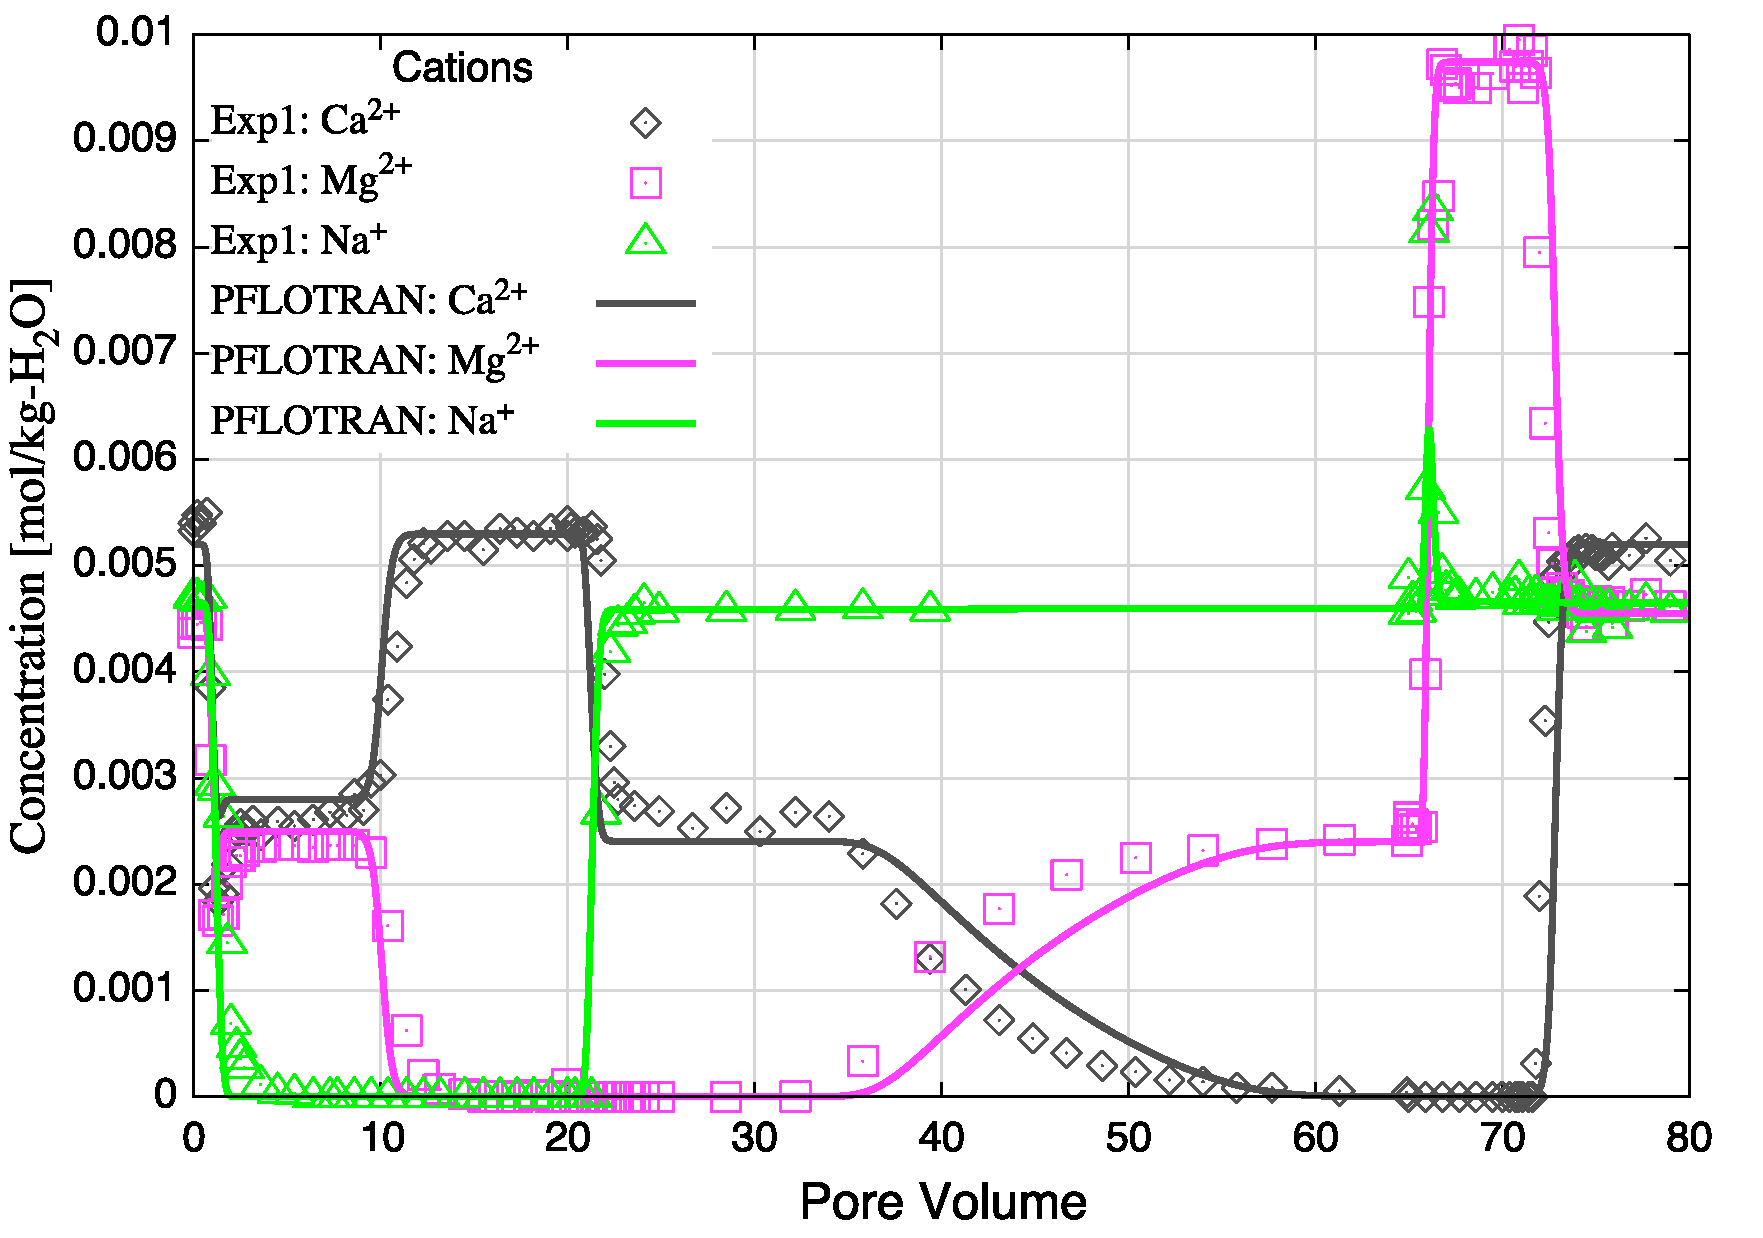
\includegraphics[scale=0.5]{./figs/ionex}
\caption{Breakthrough curves for Ca$^{2+}$, Mg$^{2+}$ and Na$^+$ compared with experimental results from Voegelin et al. (2000).}\label{fionex}
\end{figure}

\newpage
\footnotesize
\verbatiminput{./inputfiles/ionex.in}\label{tionex}
\normalsize

\newpage

\subsection{SX-115 Hanford Tank Farm}

\subsubsection{Problem Description}

The saturation profile is computed for both steady-state and transient conditions in a 1D vertical column consisting of a layered porous medium representing the Hanford sediment in the vicinity of the S/SX tank farm. The transient case simulates a leak from the base of the SX-115 tank. This problem description is taken from Lichtner et al. (2004).

\subsubsection{Governing Equations}

The moisture profile is calculated using parameters related to the Hanford sediment at the S/SX tank farm based on the Richards equation for variably saturated porous media. The Hanford sediment is composed of five layers with the properties listed in Tables~\ref{t1} and \ref{t2}. The governing equations consist of Richards equation for variably saturated fluid flow given by
\EQ
\frac{\p}{\p t} \varphi s\rho + \bnabla\cdot\bq\rho \eq Q,
\EN
and solute transport of a tracer
\EQ
\frac{\p}{\p t}\varphi C + \bnabla\cdot\big(\bq C - \varphi s \tau D \bnabla C\big) \eq Q_C.
\EN
In these equations $\varphi$ denotes the spatially variable porosity of the porous medium assumed to constant within each stratigraphic layer, $s$ gives the saturation state of the porous medium, $\rho$ represents the fluid density in general a function of pressure and temperature, $C$ denotes the solute concentration, $D$ denotes the diffusion/dispersion coefficient, $\tau$ represents tortuosity, $Q$ and $Q_C$ denote source/sink terms, and $\bq$ denotes the Darcy velocity defined by
\EQ
\bq\eq - \frac{k_{\rm sat}k_r}{\mu} \bnabla (p-\rho g z),
\EN
with saturated permeability $k_{\rm sat}$, relative permeability $k_r$, fluid viscosity $\mu$, pressure $p$, formula weight of water $W$, acceleration of gravity $g$, and height $z$. Van Genuchten capillary properties are used for relative relative permeability according to the relation
\EQ\label{kr}
k_{r} \eq \sqrt{s_{\rm eff}} \left\{1 - \left[1- \left( s_l^{\rm 
eff} \right)^{1/m} \right]^m \right\}^2, 
\EN
where $s_{\rm eff}$ is related to capillary pressure $P_c$ by the equation
\EQ\label{sat}
s_{\rm eff} \eq \left[1+\left( \alpha |P_c| \right)^n 
\right]^{-m}, 
\EN 
where $s_{\rm 
eff}$ is defined by 
\EQ\label{seff1}
s_{\rm eff} \eq \frac{s - s_r}{1 - s_r}, 
\EN 
and where $s_r$ denotes the residual saturation. The quantity $n$ is related to $m$ by the expression 
\EQ\label{lambda} 
m \eq 1-\frac{1}{n}, \ \ \ \ \ n \eq \frac{1}{1-m}. 
\EN 
The capillary pressure $P_c$ and fluid pressure $p$ are related by the (constant) gas pressure $p_g^0$
\EQ
P_c \eq p_g^0-p,
\EN
where $p_g^0 \!=\! 101,325$ Pa is set to atmospheric pressure.

\paragraph{Semi-Analytical Solution for Steady-State Conditions}

For steady-state conditions the saturation profile satisfies the equation
\EQ
\frac{d}{dz} \rho q_z \eq 0,
\EN
or assuming an incompressible fluid
\EQ
q_z \eq q_z^0,
\EN
where $q_z^0$ denotes infiltration at the surface. Thus the pressure is obtained as a function of $z$ by solving the ODE
\EQ\label{dpdz}
\frac{dp}{dz} \eq -\frac{\mu q_z^0}{k_{\rm sat} k_r} - \rho g,
\EN
using Eqns.\eqref{kr} and \eqref{sat} to express the relative permeability $k_r$ as a function of pressure. For the special case of zero infiltration it follows that
\EQ
p(z) \eq p_0 - \rho g (z-z_0),
\EN
with $p(z_0)\!=\!p_0$. The saturation profile is obtained from Eqns.\eqref{sat} and \eqref{seff}.

\paragraph{Watertable}

The position of the watertable is defined by vanishing of the capillary pressure
\EQ
P_c(z_{\rm wt}) \eq 0,
\EN
where $z_{\rm wt}$ denotes the height of the watertable. For the case with no infiltration at the surface it follows that
\EQ
z_{\rm wt} \eq z_0 + \frac{p_0-p_g}{\rho g},
\EN
with the boundary condition $p(z_0) = p_0$ and $z_0$ denotes the datum. If $p_0$ is set equal to $p_g$, then $z_{\rm wt} = z_0$, or the height of the watertable is equal to the datum.
The same holds true also with constant nonzero infiltration. 

\begin{comment}
To see this note that the pressure satisfies Eqn.\eqref{dpdz}. Integrating this equation yields
\EQ
p(z) \eq p_0 - \rho g (z-z_0) -\frac{\mu q_z^0}{k_{\rm sat}} \int_{z_0}^z \frac{dz'}{k_r}.
\EN
Thus the watertable is determined implicitly from the equation
\EQ\label{wt}
z_{\rm wt} \eq z_0 + \frac{p_0 -p_g}{\rho g} + \frac{\mu q_z^0}{\rho g k_{\rm sat}} \int_{z_0}^{z_{\rm wt}} \frac{dz}{k_r}.
\EN
Note that if $z_{\rm wt} = z_0$, the integral on the right-hand side vanishes.
Expanding the integral on the right-hand side yields
\BA
\int_{z_0}^{z_{\rm wt}} \F dz' &\eq \frac{\G_0}{\rho g} \int_{z_0}^{z_{\rm wt}} \Big[\F_0 + \frac{1}{1!}\F_0' z' + \frac{1}{2!} \F_0'' (z')^2 + \cdots \Big] dz',\\
&\eq \frac{\G_0}{\rho g} \Big[\F_0 (z_{\rm wt}-z_0) + \frac{1}{1! 2}\F_0' (z_{\rm wt}^2-z_0^2) + \frac{1}{2! 3} \F_0'' (z_{\rm wt}^3-z_0^3) + \cdots  \Big].
\EA
Consequently, it is clear that for $p_0=p_g$, $z_{\rm wt}=z_0$ satisfies Eqn.\eqref{wt}. For $p_0\ne p_g$, the watertable height depends on $q_z^0$.
\end{comment}

\subsubsection{Model Parameters}

Model parameters used in the simulations are listed in Tables~\ref{t1} and \ref{t2}. Although not needed here, thermal properties are also listed. Diffusivity was set to $10^{-9}$ m$^2$ s$^{-1}$ and tortuosity was set to one.

\renewcommand{\tabcolsep}{1.7mm}

\begin{table}[H]\centering
\caption{Stratigraphic sequence used in the calculations, after Ward et al. (1996).}\label{t1}

\vspace{3mm}

\begin{tabular}{lcr}
\toprule
Formation & Abbrev. & Thickness [m]\\
\midrule
Backfill & BF & 16.0\\
Hanford Fine Sand & HF & 23.0\\
Plio-Pleistocene & PP & 6.0\\
Upper Ringold Gravel & URG & 3.0\\
Middle Ringold Gravel & MRG & 20.0\\
\bottomrule
\end{tabular}
\end{table}

\begin{table}[H]\centering
\caption{Parameters for material and thermal properties for intrinsic rock density $\rho_s$, heat capacity $c$, thermal conductivity $\kappa$, porosity $\varphi$, residual water saturation $s_r$, van Genuchten parameters $\alpha$ and $\lambda$, and vertical water saturated permeability $k_{\rm sat}$. Data taken from Khaleel and Freeman (1995), Khaleel et al. (2001), and Pruess et al. (2002).}\label{t2}

\vspace{3mm}

\begin{tabular}{lccccccccc}
\toprule
Formation & $\rho_s$ & $c$ & $\kappa_{\rm dry}$ & $\kappa_{\rm wet}$ & $\varphi$ & $s_r$ & $\alpha$ & $m$ & $k_{\rm sat}$\\
& g cm$^{-3}$ & J kg$^{-1}$ K$^{-1}$ & \multicolumn{2}{c}{W m$^{-1}$} & --- & --- & Pa$^{-1}$ & --- & m$^2$\\
\midrule
BF  & 2.8 & 800 & 0.5 & 2 & 0.2585 & 0.0774 & 1.008e-3 & 0.6585  &1.240e-12\\
HF  & 2.8 & 800 & 0.5 & 2 & 0.3586 & 0.0837 & 9.408e-5 & 0.4694  &3.370e-13\\
PP  & 2.8 & 800 & 0.5 & 2 & 0.4223 & 0.2595 & 6.851e-5 & 0.4559  &3.735e-14\\
URG & 2.8 & 800 & 0.5 & 2 & 0.2625 & 0.2130 & 2.966e-5 & 0.3859  &1.439e-13\\
MRG & 2.8 & 800 & 0.5 & 2 & 0.1643 & 0.0609 & 6.340e-5 & 0.3922  &2.004e-13\\
\bottomrule
\end{tabular}
\end{table}

\subsubsection{Simulation Results}

The calculations are carried out for an isothermal system using Richards equation. First, the steady-state saturation profile is obtained without the tank leak present. Then using the steady-state profile as the initial condition the tank leak is turned on. The results for the steady-state saturation and pressure profiles are shown in Figure~\ref{f1} for infiltration rates at the surface of 0, 8 and 80 mm/y. The mean infiltration rate at the Hanford site is approximately 8 mm/y. A 1D column 68 m heigh with the water table located at a height of 6 m from the bottom is used in the simulation. A uniform grid spacing of 0.5 m is used to discretize Richards equation.

Shown in Figure~\ref{f2} is the saturation at different times following a two week leak releasing 60,000 gallons from the SX-115 tank at a depth of 16 m. In the simulation a release rate of $1.87\!\times\! 10^{-3}$ kg/s is used.


\clearpage

\begin{figure}[h]\centering
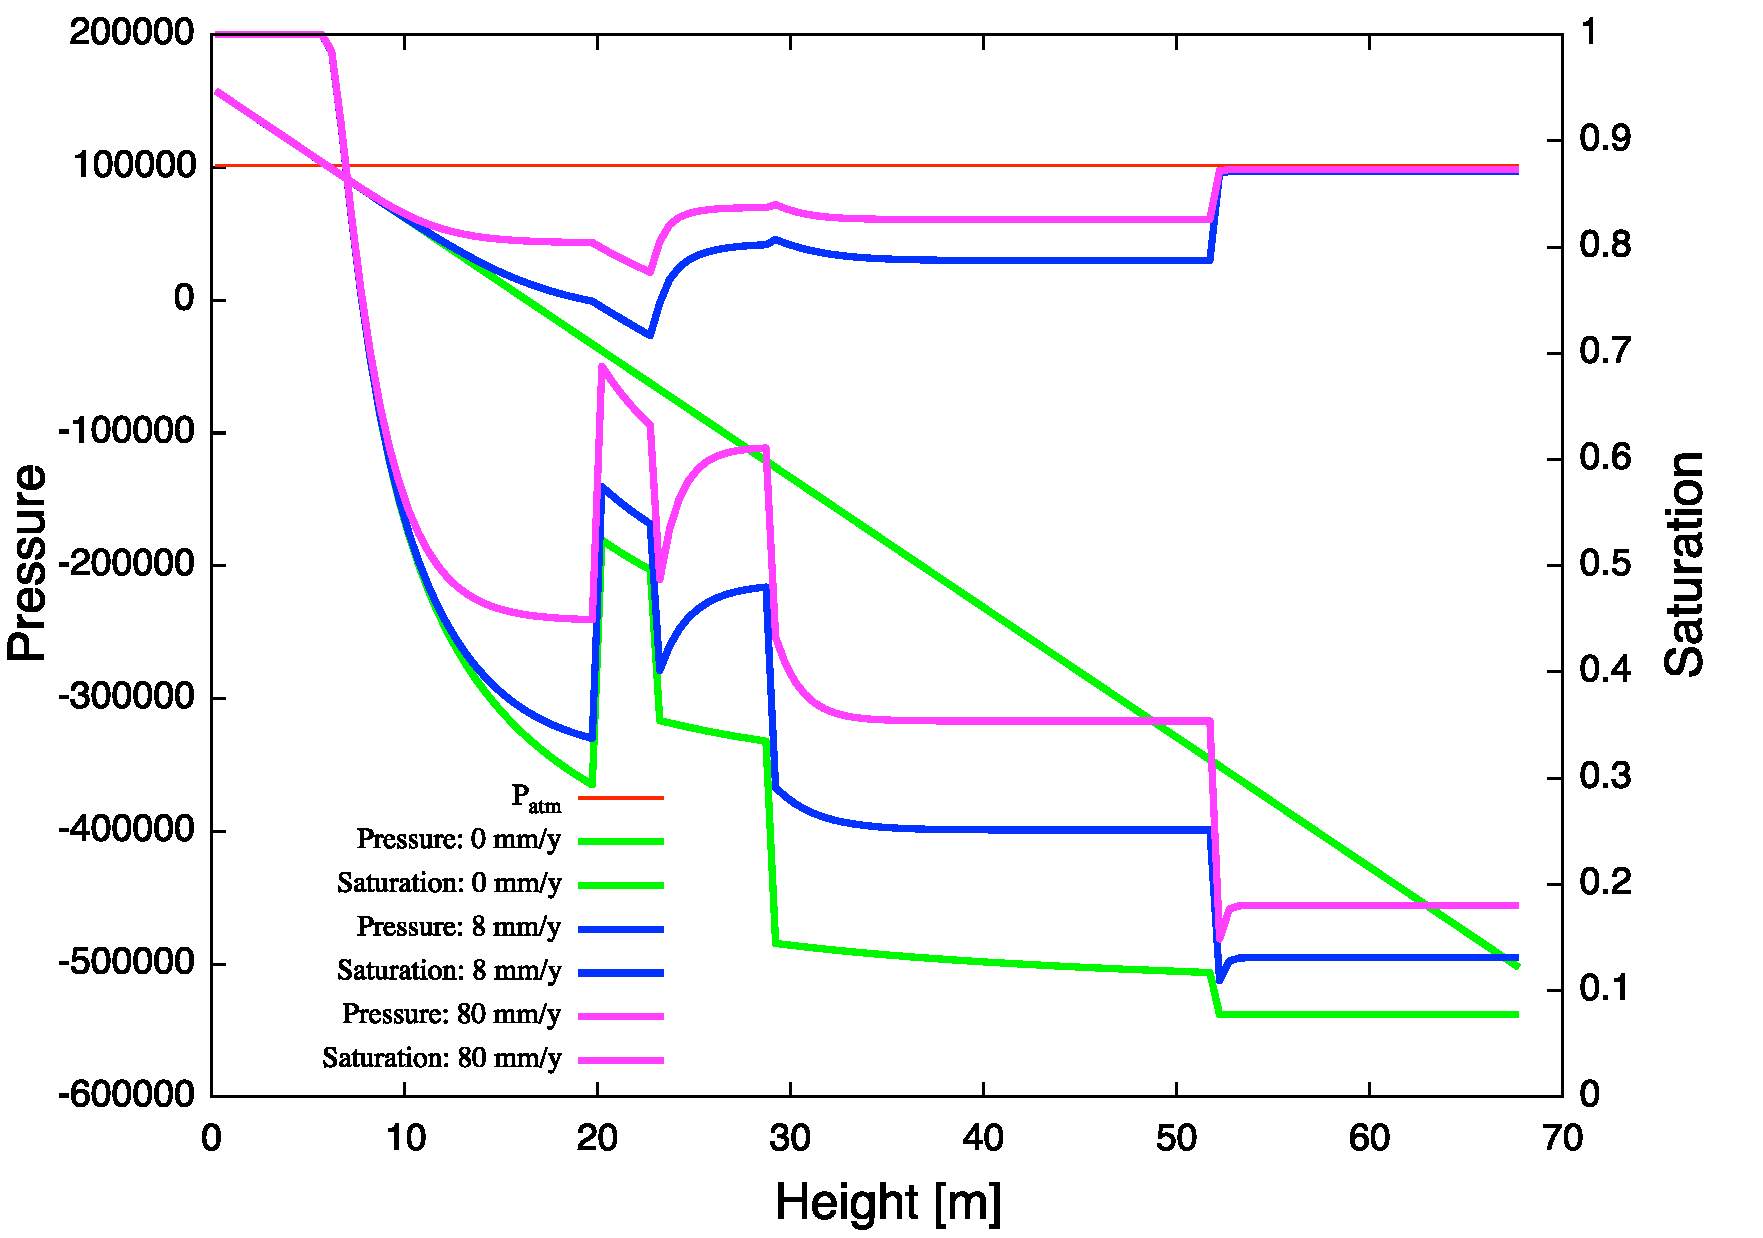
\includegraphics[scale=0.45]{./figs/ps}
\caption{Steady-state saturation and pressure profiles for infiltration rates of 0, 8 and 80 mm/y. The water table is located at 6 m from the bottom of the computational domain.}\label{f1}
\end{figure}

\begin{figure}[h]\centering
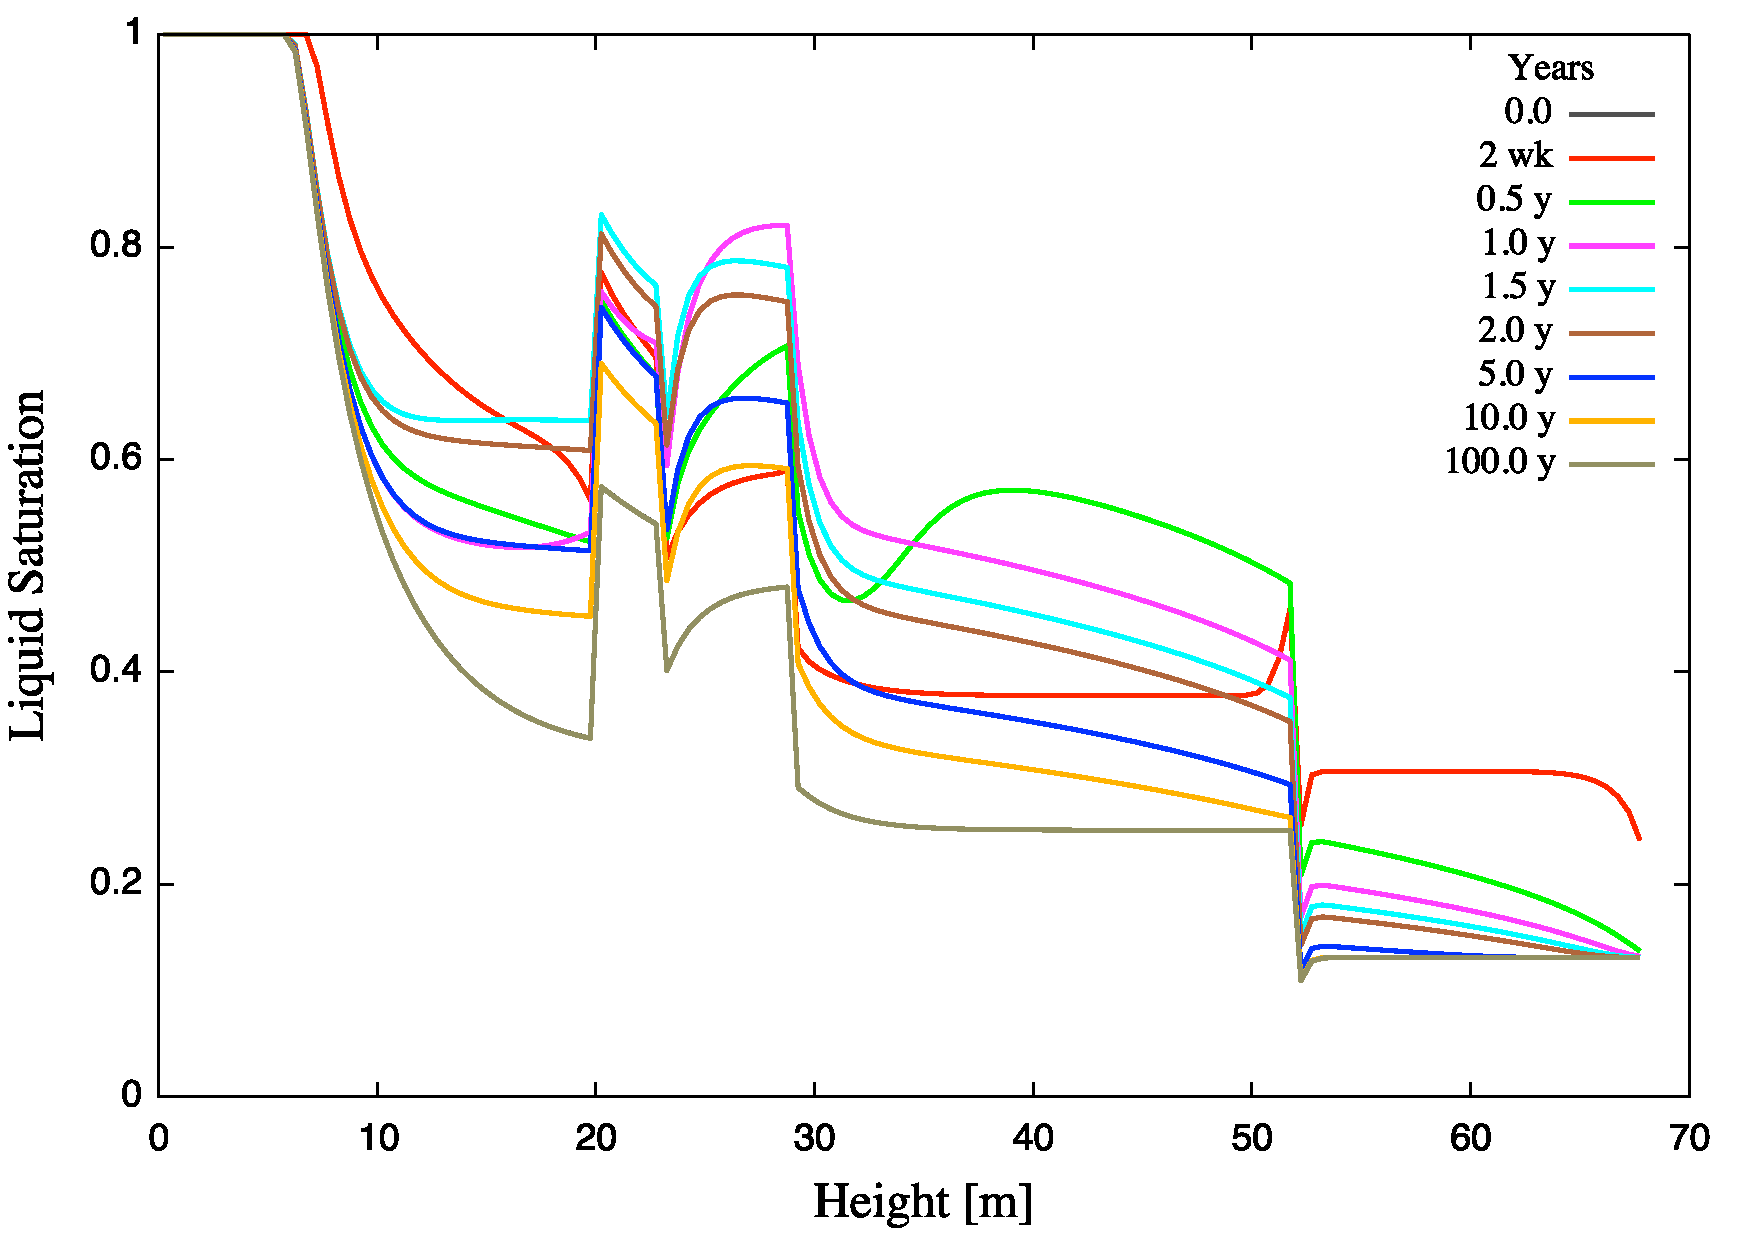
\includegraphics[scale=0.45]{./figs/sat_leak}
\caption{Simulation of a tank leak with a duration of two weeks showing the saturation profile for different times indicated in the figure.}\label{f2}
\end{figure}

\begin{figure}[h]\centering
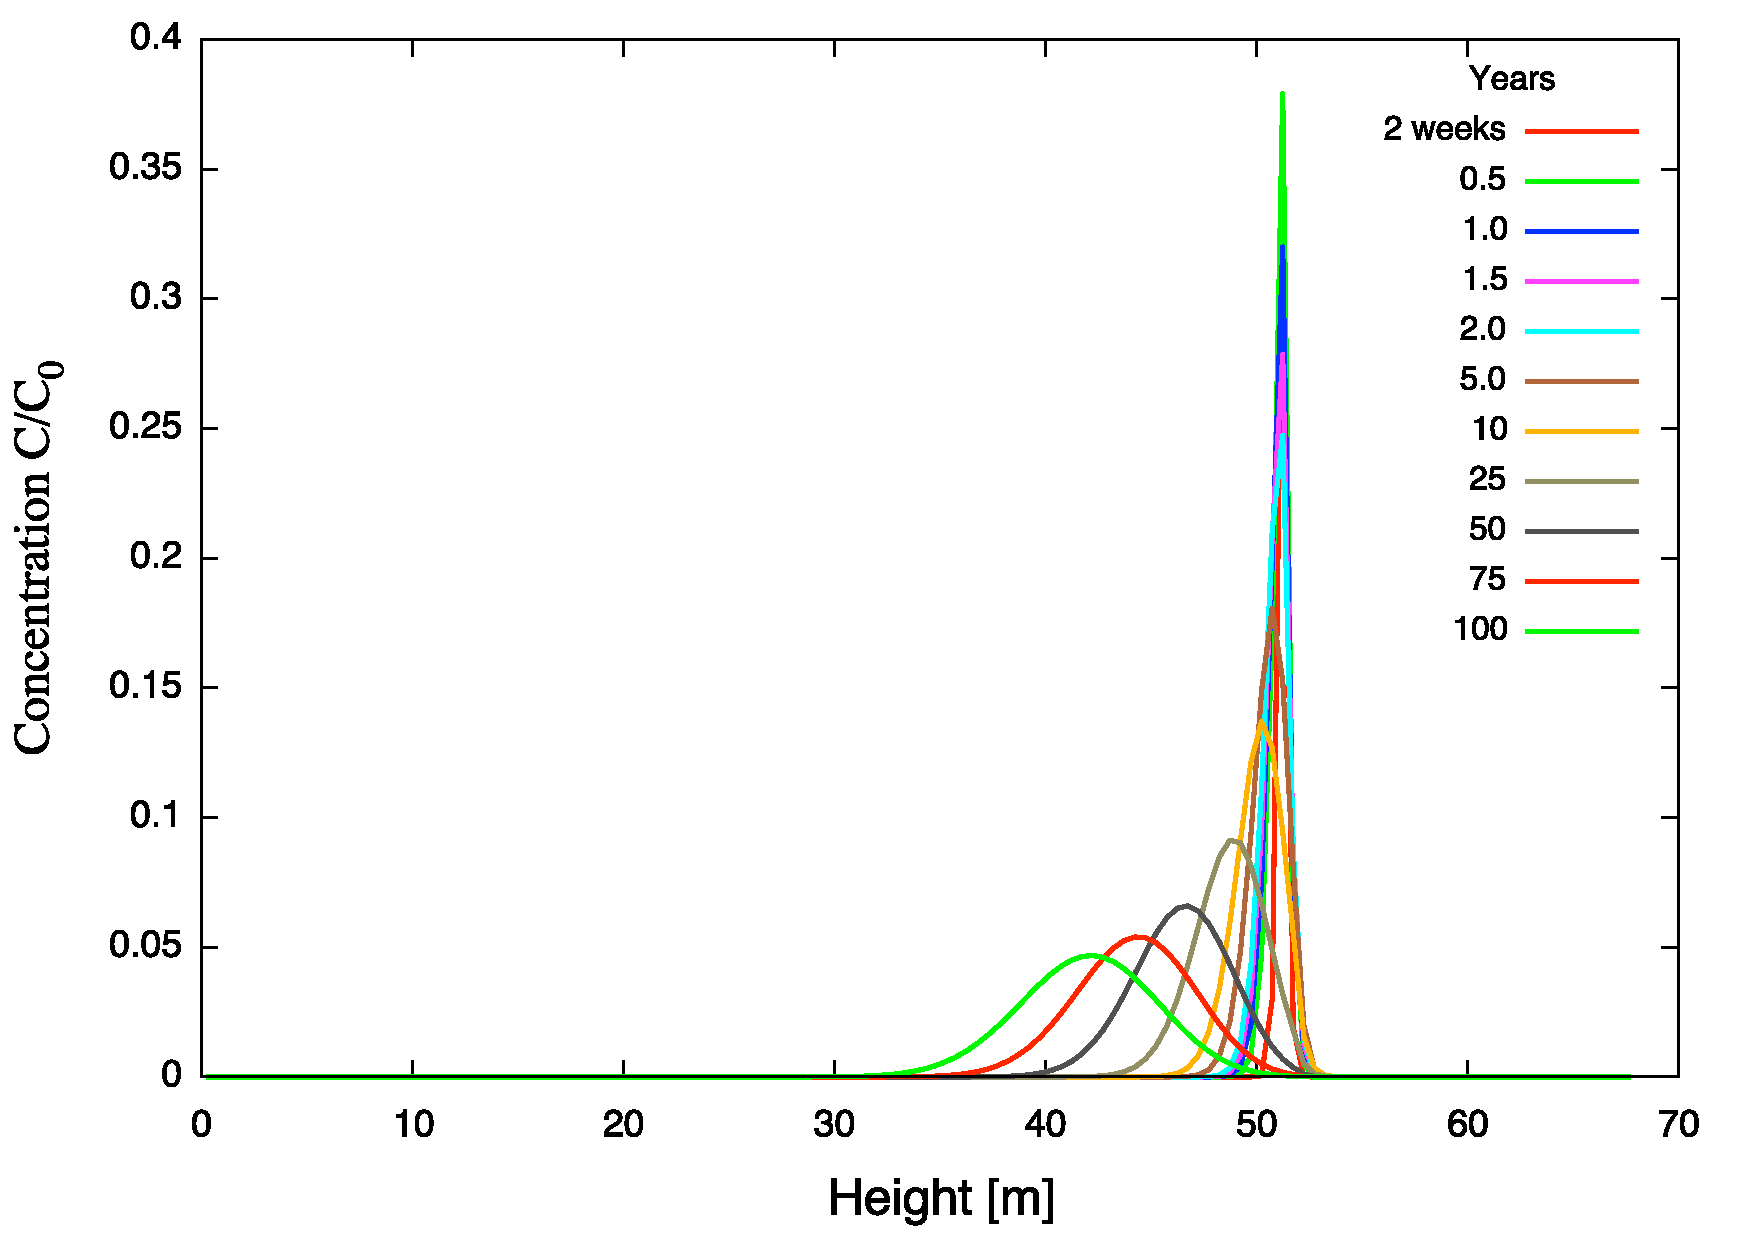
\includegraphics[scale=0.45]{./figs/conc}
\caption{The solute concentration profile corresponding to Figure~\ref{t2} for different times indicated in the figure.}\label{f3}
\end{figure}

\clearpage

\subsubsection{PFLOTRAN Input Files}

Listing of PFLOTRAN input file including a tracer. Note that the stratigraphic zone specification in {\tt REGION} is grid independent as is the grid size specification in keyword {\tt GRID}. Therefore to change the grid spacing only the line: {\tt NXYZ 1 1 136}, needs to be changed. Also note that a line beginning with a colon (:) is read as a comment.

\bigskip

\noindent PFLOTRAN input file {\tt pflotran.in}: 
\footnotesize
\verbatiminput{./inputfiles/sx115/sx115.in}

\clearpage

\normalsize
\noindent
Source/sink file {\tt src.dat}:
\footnotesize
\verbatiminput{./inputfiles/sx115/src.dat}
\normalsize


\section{References}

\begin{description}

\item Balay S, Eijkhout V, Gropp WD, McInnes LC and Smith BF (1997) Modern Software Tools in Scientific Computing, Eds. Arge E, Bruaset AM and Langtangen HP (Birkha\"user Press), pp. 163--202.

\item Coats, K.H. and A.B. Ramesh (1982) Effects of Grid Type and Difference Scheme on Pattern Steamflood Simulation Results, paper SPE-11079, presented at the 57th Annual Fall Technical Conference and Exhibition of the Society of Petroleum Engineers, New Orleans, LA, September 1982.

\item Goode, D.J. (1996) Direct simulation of groundwater age, Water Resources Research, 32, 289--296.

\item Hammond, G.E., P.C. Lichtner, C. Lu, and R.T. Mills (2011) PFLOTRAN: Reactive Flow \& Transport Code for Use on Laptops to Leadership-Class Supercomputers, Editors: Zhang, F., G. T. Yeh, and J. C. Parker, {\em Ground Water Reactive Transport Models}, Bentham Science Publishers. ISBN 978-1-60805-029-1. 

\item Khaleel, R., E.J. Freeman (1995) Variability and scaling of hydraulic properties for 200 area soils, Hanford Site. Report WHC-EP-0883. Westinghouse Hanford Company, Richland, WA.

\item Khaleel, R., T.E. Jones, A.J. Knepp, F.M. Mann, D.A. Myers, P.M. Rogers, R.J. Serne, and M.I. Wood (2000) Modeling data package for S-SX Field Investigation Report (FIR). Report RPP-6296, Rev. 0. CH2M Hill Hanford Group, Richland, WA.

\item Lichtner, P.C., Yabusaki, S.B., Pruess K., and Steefel, C.I. (2004) Role of Competitive Cation Exchange on Chromatographic Displacement of Cesium in the Vadose Zone Beneath the Hanford S/SX Tank Farm, {\em VJZ}, {\bf 3}, 203--219.

\item Lichtner P.C. (2000)  Critique of Dual Continuum Formulations of Multicomponent Reactive Transport in Fractured Porous Media, Ed. Boris Faybishenko, {\em Dynamics of Fluids in Fractured Rock}, Geophysical Monograph {\bf 122}, 281--298.

\item Peaceman, D.W. (1977) Interpretation of Well-Block Pressures in Numerical Reservoir Simulation with Nonsquare Grid Blocks and Anisotropic Permeability, paper SPE-10528, presented at the Sixth SPE Symposium on Reservoir Simulation of the Society of Petroleum Engineers, New Orleans, LA, January 1982.  

\item Pruess, K., S. Yabusaki, C. Steefel, and P. Lichtner (2002) Fluid flow,
heat transfer, and solute transport at nuclear waste storage tanks in the Hanford vadose zone. Available at www.vadosezonejournal.org. Vadose Zone J. 1:68--88.

\item Pruess, K., and Narasimhan (1985) A practical method for modeling fluid and heat flow in fractured porous media, SPE 10509, 14--26.

\item Somerton, W.H., A.H. El-Shaarani, and S.M. Mobarak (1974) 
High temperature behavior of rocks associated with geothermal-type reservoirs. Paper SPE-4897. Proceedings of the 44th Annual 
California Regional Meeting of the Society of Petroleum Engineers. Richardson, TX: Society of Petroleum Engineers. 

\item Andreas Voegelin, Vijay M. Vulava, Florian Kuhnen, Ruben Kretzschmar (2000) Multicomponent transport of major cations predicted from binary adsorption experiments, Journal of Contaminant Hydrology, 46, 319--338.
\end{description}

\end{document}

